% ME310 Report Template -- Started 28 July 2006  Mark Cutkosky
% Updated: 7Aug08 -LMS; 25Nov10 Mark Cutkosky
% Updated with some new sections 4Dec2012 Mark Cutkosky
% Minor changes for 2013-14 13Nov2013 -- Mark C.
%%%%%%%%%%%%%%%%%%%%%%%%%%%%%%%%%%%

% Rename this file to whatever you like (e.g. OurFallDoc.tex) and modify the title, authors
% etc. below. If you rename the section files (e.g. Ch2context.tex) you'll need to change
% the \include{ } calls in this document as well.

%%%%%%%%%BEGIN DOCUMENT STYLE SETTINGS%%%%%%%%%%%
% Don't modify this stuff unless you know what you're doing...
% We are using the "memoir" class, a widely used set of macros book-like documents.
% If you get errors that you are missing the "memoir" package you can download and 
% install it:   http://www.ctan.org/tex-archive/macros/latex/contrib/memoir/

% memoir document class for standard USA letter paper, printed one side
\documentclass[11pt,letterpaper,oneside]{memoir}
\chapterstyle{section}
%\pagestyle{companion}    % If you want fancier page headers 
\usepackage{graphicx}        % standard LaTeX graphics 
\usepackage{color}               % support for colored fonts
\usepackage{url}  \urlstyle{same}     % deal with url strings in bibliography

\usepackage[final]{pdfpages}

%Optional fonts if you don't like the default in Latex
%\usepackage[T1]{fontenc}
%\usepackage{mathptmx}  %This will give you Times Roman, like default in MS Word.
%\usepackage{charter}       %This will give you a slightly bolder Charter font 

%More special packages to help deal with long requirements tables 
%that might span multiple pages.
\usepackage{multirow} %deal with merged cells in tables
\usepackage{supertabular}
\usepackage{longtable}
\usepackage{morefloats}
\usepackage[ampersand]{easylist}

\usepackage[pdftex,           %hyperlink cross references, etc.
    pdfsubject={ME310 Documentation},
    colorlinks={true},
    linkcolor={black},
    citecolor={blue},
    bookmarksopenlevel=1,
]{hyperref}

%The file "me310.sty" should be in the same directory as this file.
% It contains formatting for page setup, titlepage, glossary, references, etc.
\usepackage{me310}
%%%%%%%END DOCUMENT STYLE SETTINGS%%%%%%%%%%


%%%%%%%%%%BEGIN TITLE PAGE%%%%%%%%%%%%%%%%
%Replace the strings below with what's right  for you.

%%Insert your Document Title here. Use \\ to force a newline.
\title{Redesigning the Flying Experience for Passengers with Limited Mobility}

%\team{Embraer} 		% Insert your Team Project Name here.

%% Insert Fall, Winter, Spring here:
%\quarter{Winter Quarter}

%%Enter your local + global team members' names here:
%\author{  
%   Rodrigo Aquino, Clifford Bargar, Maria Barrera, Luiz Dur\H{a}o, \\
%  Laura Hoinville, Guilherme Kok, Amanda Mota
% } % end authors       

%% If you don't want it to use the printing date, replace "\today"
%% with the date that you want.
%\date{\today}
%%%%%%%%%%%END TITLE PAGE%%%%%%%%%%%%%


%%%%%%%%%BEGIN ANY CUSTOM ABBREVIATIONS%%%%%%
% Define any abbreviations that will apply throughout the document
% to save typing. Examples:
\def\pmt{{\em Papier M\^{a}ch\`{e}}}  %Define "\pmt" to print "Papier Mache" with accents +1space
\def\cbike{{\em Casterbike} \,}  %Define "\cbike" to print "Casterbike " italicized +1space
%%%%%%%%%END CUSTOM ABBREVIATIONS%%%%%%%%%

%%%%%%%%DRAFT COMMENTS%%%%%%%%%%%%%%%%
%Allow comments (remarks) to be shown or hidden.
% Put optional text in \begin{remark} ... \end{remark}  environments.
%The usage is a bit counterintuitive: \commentsoff makes them visible; \commentson hides them.
%\commentson{remark} %Don't print remarks.
\commentsoff{remark}  %Do print remarks. 


%%%%%%%%%%%%%%%%%%%%%%%%%%%%%%%%%%%%%%%%
%   BEGIN THE MAIN DOCUMENT
%%%%%%%%%%%%%%%%%%%%%%%%%%%%%%%%%%%%%%%%
\begin{document}

%If you want a figure on the cover page, this is where it goes.
%7 cm is about max figure height before messing up title spacing.
%If making your own fancy coverpage (e.g. in Photoshop) then comment out 
%the \includegraphics{ } and use the \vspace{ } command.
%\begin{figure}[t]
%\centering
  %An example cover image, from 2008 ME310 Kodak project
%  \includegraphics[height= 7cm]{images/Top_Photo.jpg}
%\vspace{3 cm}    %Use this instead when you have no cover picture 
%\end{figure}

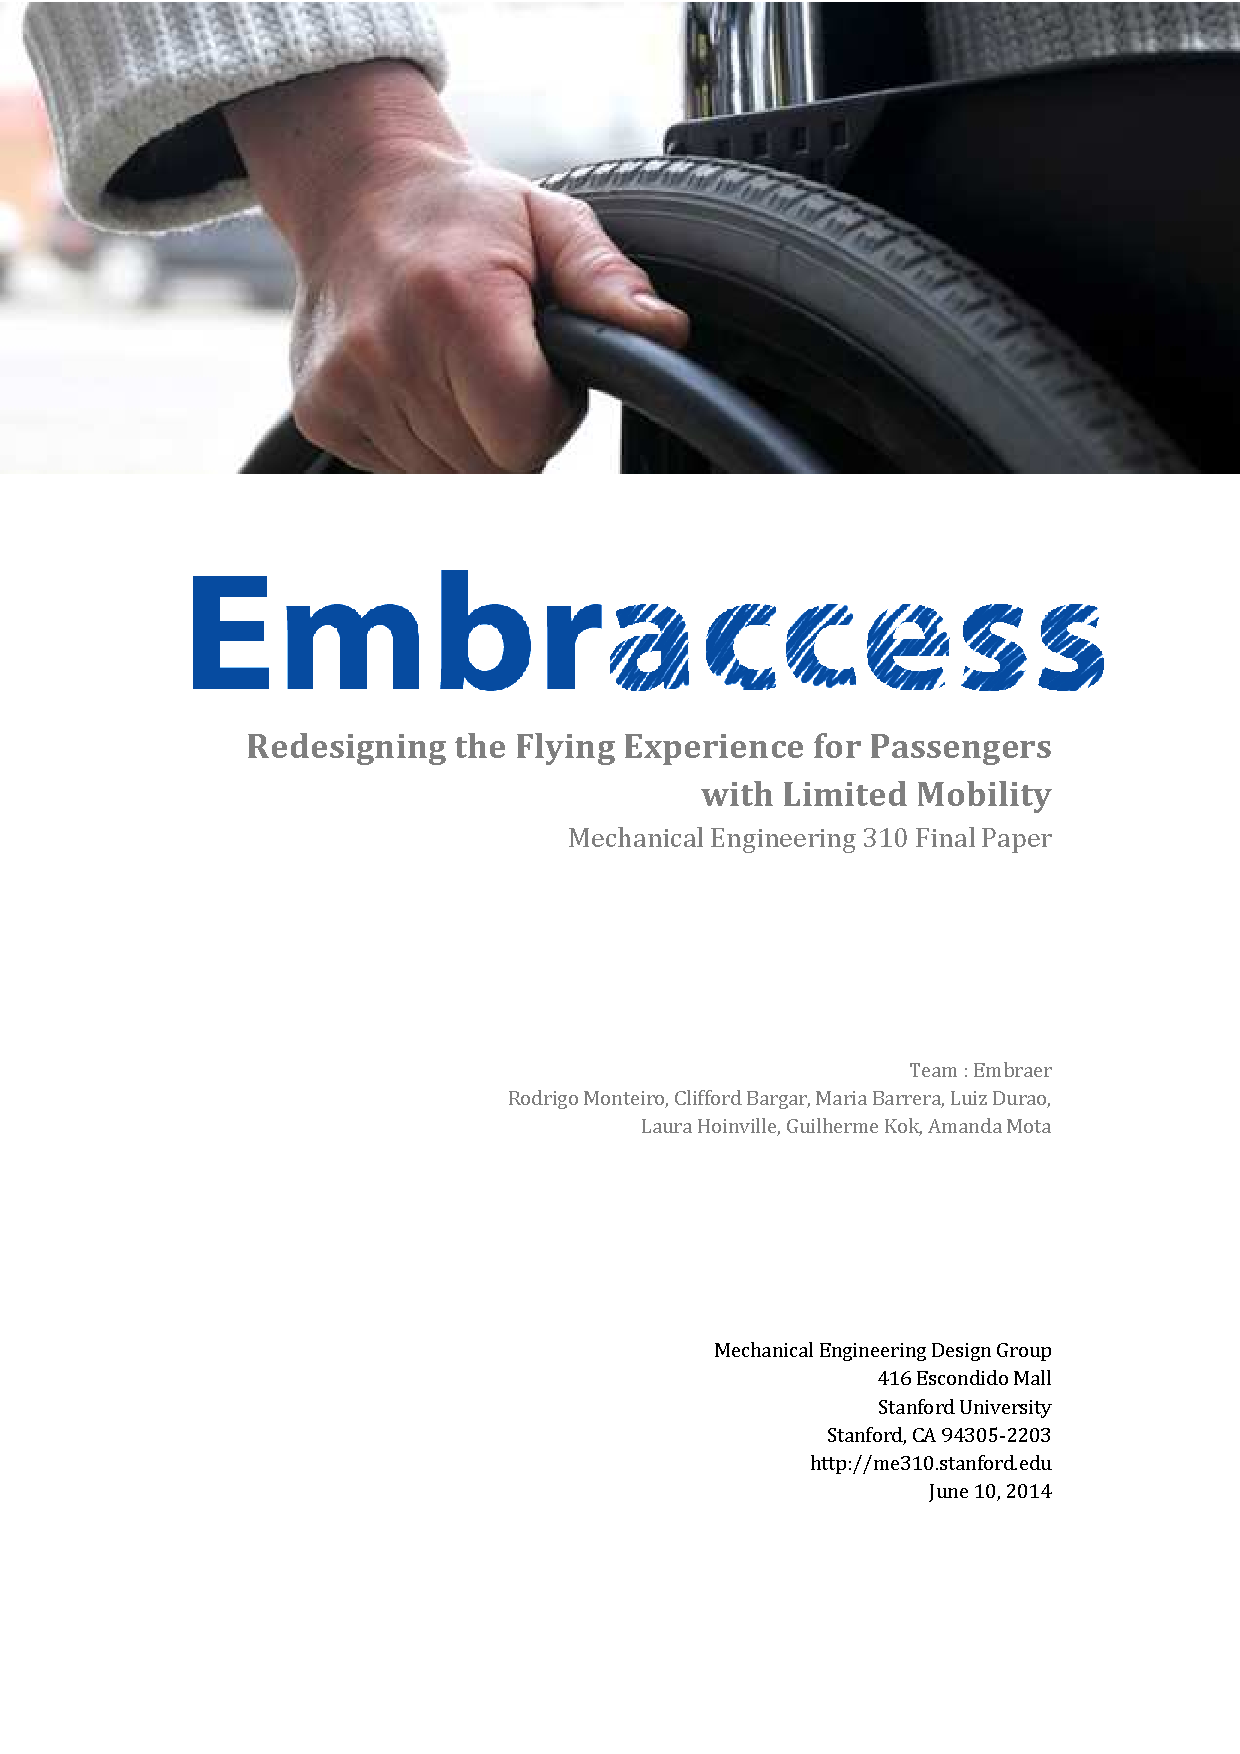
\includepdf[fitpaper=true]{Cover}

%The executive summary is a special chapter before the TOC
% See the other sections (e.g. Context) for more normal chapter headings
%%%%%%%%%%%%%%%%%%%%%%%%%%%%%%%%%%%%
% Call it Front Matter in TOC, as it will include Glossary and auto-generated TOC, LOF.
\chapter[Front Matter]{Front Matter}
\label{cha:front}
\addcontentsline{toc}{section}{Executive Summary}
%%%%%%%%%%%%%%%%%%%%%%%%%%%%%%%%%%%%
%Begin the actual executive summary text. If you create any subsections you
%probably want to use  \section*{Section name}  with an asterisk, so they are not numbered.
% Note: to get proper looking quotes use two left/right single quotes: ``. . . ''

%Example of a remark that can be optionally printed:In a world that is dynamic in almost every aspect, mobility is a necessity.  However, for persons that suffer from disabilities, their mobility may be limited.  Traveling with limited mobility can be a very difficult and burdening task especially if the travelling involves being within the small confines of an airplane.  Passengers that are faced with limited mobility or a disability have a different and often times worse experience than the average passenger during the entire flight experience.  How can have all passengers have the same experience? Designing a new futuristic cabin and creating a new travel system are essential for achieving the same experience for all passengers and to give passengers with limited mobility independence and control.

Embraer, the Brazilian airline manufacturer, decided to partner with Stanford University and the University of Sao Paulo to approach this problem of improving the entire air travel experience for persons with limited mobility. In collaboration, we started this journey toward a solution through extensive needfinding and benchmarking. The needfinding centered on conducting user interviews for both the disabled passenger and the flight crew while benchmarking focused on analogous situations, patents, regulations, and current concepts and solutions.

The research that was conducted during needfinding and benchmarking was instrumental in the approach we are taking toward a solution. The user interviews led us to the five themes we need to address with our solution. These themes are customer service, control, independence, seat preferences, and non-discriminatory. \ref{fig:main_themes} shows the themes and how they each rely on the others to be successful. The interviews with potential users revealed horror stories that dealt with customer service or the lack thereof. The solution space needs to create an environment that limits the interaction between the flight crew and the passenger to prevent these horror stories from becoming a reality for future travelers. Independence and control were also instrumental in our findings. The users of our solution want to feel independent and in control of their situation even though they might need assistance. This leads our solution path to one that provides piece of mind to our user. Because wheelchairs often gets damaged when they are handled from the jet way to the cargo hold, wheelchair users are very anxious and spend their flight wondering if once arrived at their final destination they will be able to use their mobility device or not. Because of their situation, limited mobility passengers and passengers with disabilities have a condition that singles them out and makes their flying experience worse than normal to begin with so why should our design add insult to injury by singling them out more? We are focusing on a universal design that would aid and improve the experience for both the limited mobility passenger and the average passenger.


These themes were our driving forces for the critical function and critical experience prototypes we created to further explore our problem space. The team created a number of prototypes but really focused on the ones that solved this problem; one being a more incremental fix while the other addressed a more futuristic solutions. 

\begin{figure}[h]
  \centering
     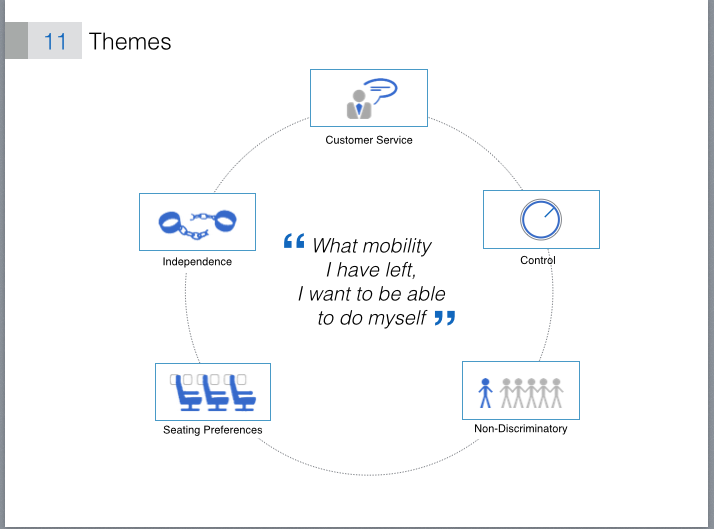
\includegraphics[width=7cm]{images/image007.png}
   \caption{Main themes driving our solution}
  \label{fig:main_themes}
\end{figure}

Our vision for a solution is a more dynamic cabin that allows the user to customize the space to his needs and allows for a more enjoyable and interactive experience. We want to change the way a passenger looks at the flying experience and how they feel before, during, and after the flight. The passengers should have more control over their seat and the way they access them. Giving passengers more independence and control while minimizing customer service interaction and discrimination is our motivation for a futuristic cabin. But beyond the idea of a futuristic cabin, airport logistics concerning wheelchair storage must also be improved. If once disabled passengers reach their final destination their wheelchair is broken then no matters how delightful their flight experience was, they will still have to face a very hard time trying to get their mobility device repaired.

In order to provide wheelchair users with an enjoyable flying experience from beginning to end, our solution must provide them with first absolute piece of mind concerning what happens to their mobility device when it is taken away from them, and second a pleasant cabin experience that makes them feel independent, in control and not singled out. Both improvements are necessary to change wheelchair users' perception of flying to their final destination at any place in the world.



%\section*{Glossary}

%\begin{list}{-}{}

%\end{list}

% Set up the Glossary. The template is looking for a file called
% "glossaryterms.tex" with glossary terms and definitions.
% You can either edit this file manually or you
% can use the Memoir glossary feature in which you insert items like
%   \glossary{glossary term}{our definition of what the term means}
% wherever you like, as you write your documentation.
% When you run the report through Latex, it will create a ".glo" file like
% "OurFallDocument.glo" which you can edit to create the file "glossaryterms.tex"
% There is also perl script I made which will do the formatting for you. 
%  perl Glo2Tex OurFallDocument.glo > glossaryterms.tex

\newpage
\section*{Glossary}
\addcontentsline{toc}{section}{Glossary}
\label{sec-glossary}
\begin{description}
  \item  \textbf{80/20:} Aluminum T-slotted profiles used for building modular structures. 

\item  \textbf{ADA:} Americans with Disabilities Act; one of America's most comprehensive pieces of civil rights legislation that prohibits discrimination against and guarantees people with disabilities have the same opportunities as everyone else to participate in the mainstream of American life.

 \item \textbf{Aisle Chair:} Common assistive device utilized to help individuals with mobility limitations to more easily board airplanes. Aisle chairs are narrower wheelchairs which highlight multiple straps to completely secure the user, and can be rolled down narrow airplane aisles to get the individual to his or her seat. 

  \item \textbf{Airport Personnel:} All parties involved in handling the passengers and cargo for a flight including but not limited to: flight attendants, luggage handlers, check-in personnel and other contracted helpers.

  \item \textbf{ANAC:} Agencia Nacional de Aviação Civil – Brazilian National Agency of Civil Aviation

  \item \textbf{ANSYS:} ANSYS Mechanical software is a comprehensive finite element analysis tool for structural analysis, including linear, nonlinear and dynamic studies. The engineering simulation product provides a complete set of elements behavior, material models and equation solvers for a wide range of mechanical design problems.

\item \textbf{Arduino:} A low cost and easy to use microcontroller for rapid prototyping of mechatronic and electrical systems

  \item  \textbf{Assistive Technology:} Assistive, adaptive, and rehabilitative devices for people with disabilities; promotes greater independence by enabling people to perform tasks that they were formerly unable to accomplish, or had great difficulty accomplishing.

  \item  \textbf{Benchmarking:} A standard by which something can be measured or judged.

\item \textbf{Boarding:} The process of entering the airplane.

  \item  \textbf{Cabin:} The section of an aircraft in which passengers travel. 

 \item  \textbf{Cargo Hold:}  The space in a ship or aircraft for storing cargo such as baggage, shipping containers, animals or mobility devices. 

  \item \textbf{Control:} The power to influence or direct either people's behavior or the course of events.

  \item \textbf{Dark Horse Prototype:} A device created during the winter quarter of ME310 that was ruled out in the fall quarter or undiscovered due to being “too risky” or “to difficult to complete”; emphasizes creative out-of-the-box thinking and exploring all of the design space for the project. 

  \item \textbf{Disability:} A physical or mental condition that limits a person's movements, senses, or activities.

\item \textbf{Disembarking:} The process of exiting the airplane.

  \item \textbf{EXPE:} The Stanford design fair that is held every year at the beginning of June. During this fair, all ME 310 teams present the work they have done throughout the year and show their final prototype.

  \item \textbf{FAA:} Federal Aviation Administration; United States national aviation authority whose mission is to provide the safest, most efficient aerospace system in the world, oversees all aspects of American civil aviation.

  \item \textbf{Independence:} Freedom from outside control or support.

\item \textbf{Jetway:} A telescoping corridor that extends from an airport terminal to an aircraft, for the boarding and disembarkation of passengers.

  \item \textbf{Limited Mobility:} Mobility impairment may be caused by a number of factors, such as disease, an accident, or a congenital disorder and may be the result from neuro-muscular or orthopedic impairments. It may include conditions such as spinal cord injury, paralysis, muscular dystrophy and cerebral palsy. It may be combined with other problems as well (i.e. brain injury, learning disability, hearing or visual impairment).

  \item \textbf{Needfinding:} Discovering opportunities by recognizing the gaps in the system or the needs.

  \item \textbf{Non-Discriminatory:} Fairness in treating people without prejudice.

  \item \textbf{Pain Points:} A level of difficulty sufficient to motivate someone to seek a solution or an alternative; a problem or difficulty.

  \item \textbf{Perspective:} A particular attitude toward or way of regarding something; a point of view.

  \item \textbf{Self-Image:} The idea one has of one's abilities, appearance, and personality.


 \item \textbf{Taxiing:} The movement of an aircraft on the ground, under its own power.

  \item \textbf{Transfer:} The act of moving a wheelchair user from one chair to another. 

   % input the list "glossaryterms.tex"
\end{description}

%%%%%% Example of an optionally printed "remark"
%\begin{remark}
%\color{blue}
%It's a sign of a successful team that the glossary becomes extensive. Define any non-obvious or invented terms. For %example, if you reference something by an acronym, that might be a glossary term. Teams also coin terms to describe %design features. Define such terms here.  Don't define obvious stuff (axle, keyboard).  

%See comments in me310report.tex if you want to generate a glossary semi-automatically from tagged keywords.
%\normalcolor
%\end{remark}

%%%%%%%%%%%%%%%%%%%%%%%%
% TOC and LOF are automatically generated -- Note that sometimes have to "compile" Latex THREE
% times to update the main .aux files, the TOC etc. files, and finally the PDF output with all changes
% propagated to the printout.
% Make Table of Contents title smaller than a normal Chapter heading:
\renewcommand{\chaptitlefont}{\normalfont\Large\bfseries}
\newpage
\tableofcontents %asterisk to prevent it from getting a number

% Optional Lists of Figures and Tables:
\newpage
\listoffigures  %Note that for this you probably want to add the [short-headings] to captions.
%\listoftables  %I decided to omit the LOT in this example.

%Back to normal size for subsequent sections
\renewcommand{\chaptitlefont}{\normalfont\Huge\bfseries}
%%%%%%%%%%%%%%%%%%%%%%%%




%%%%%%%%%%%%%%%%%%%%%%%%%%%%%%%%
%% On to the main sections....  Just comment out the \input{} line
%% for any chapters that aren't ready yet.

%%%%%%%%%%%%%%%%%%%%%%%%%%%%%%%%
%MRC5December2012 -- Added a bit about  the corporate partner context
%Context
\chapter{Context}
\label{sec-context} %Label for cross-referencing

\section{Need Statement}
Airlines are always searching for new ways to fit more people on a single flight and increase their profit margin, making the seats in the aircraft smaller and closer. As the seats get smaller, the personal space for a passenger shrinks, making it harder for anyone to move and fit comfortably as shown in Figure \ref{fig:9}.

\begin{figure}[h]
  \centering
     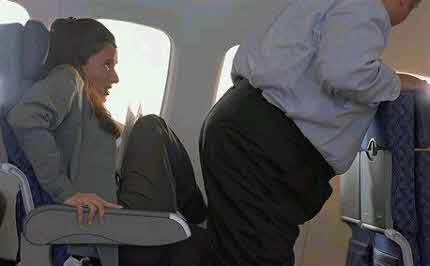
\includegraphics[width=7cm]{images/image009.png}
   \caption{With Airlines adding more and more seats to their planes, it is increasingly hard to maneuver around the cabin. \cite{2014airlines}}
  \label{fig:9}
\end{figure}


As global business continues to increase, people are constantly on the go and airports are becoming larger and larger, growing more busy each year.  The distance from check-in to gate is increasing as more airlines expand routes and terminals.    Therefore, it becomes a problem for passengers who have a hard time walking long distances or need assistance with bags or a wheelchair. More airport staff are needed to move the passengers with assistance needs, and often the staff are not trained in dealing with disabilities.  

Additionally, airlines have  limited space in the cabin because of the increased amount of seats, requiring assistive devices  to be stored in the cargo hold where they are susceptible to damage.  The flying experience today is tailored to a person that has all of his/her mobility, leaving out those who do not have the mobility or have some impairment that requires additional time. However, 58 million Americans live with a disability, including 5.5 million military veterans. %\cite{}

%Would it not be great if the flying experience were individually tailored to a person’s needs? What if the cabin could be %redesigned to improve the flying experience for the passengers with limited mobility as well as for the average passenger? %Such design would create an experience that is comfortable, making the airline and aircraft manufacturer more popular %among its customers because the final user, the passenger, is the one the plane is designed for.

\section{Problem Statement}
The need of our users or the problems facing our users can be broken down into two areas to be addressed:

\begin{list}{-}{}
  \item Mobility in the Cabin
  \item Storage and Security of Assistive Devices
\end{list}

The whole process (see Appendix – Diagram A1) was analyzed, and the current systems that are in use today are based on what is required by the FAA and ADA regulations.  However, these systems have gaps that need to fix in order to improve the user and passenger experience.  Last quarter's user interviews showed the gaps and led to these two main pain points. These two pain points of mobility within the cabin and storage and security of assistive devices address our group of users who are passengers with limited mobility that use assistive devices.  Our users want to be able to transfer from their wheelchair to the aisle chair independently and without the interference of others.  They also want to know that their wheelchair will be handled with the utmost care and returned to them in working condition with no damage at all.   This is what our user needs and wants addressed in order to have a better flying experience that is more personal, allows independence, and provides peace of mind. In addition, the airport staff and flight attendants need to be considered to ensure that they can use the new systems with ease and without increased time committment by making the solution inclusive into the flight crew's tasks.


\section{Vision Statement}

Imagine you are packing for a trip and you pack your most important possession in your carry-on.   But when you arrive at the gate, you are required to gate check your bag.  You immediately panic. You do not know if the bag will be damaged. What if it gets lost? Put on the wrong flight? Your entire flight is ruined because all you can think about is what state your bag will be when you arrive since airlines do not have the best reputation concerning luggage handling.  Now imagine if this was your wheelchair.  Your legs. Your independence. What if you had no clue how you were going to move now that you do not have your chair? What if your activity in the cabin was limited due to the loss of your chair?   For our users, this is a struggle every time they board a plane and have to endure a flight of misery and constant worry.  What if we could eliminate this unease, worry and fear by designing a new system that allows the user to put their own wheelchair into its “personal spot”, to know how it was handled, to know it was safe, and to know where it is at all times and that it will be there when they disembark?  What if we could design a way for them to be able to move in the cabin with ease and make the bathroom and other tasks more accessible? 

The two systems described in the story above are our vision and focus for the final product. Our users are in need of independence.  The current systems that are utilized today on airplanes and in airports require our users to be assisted by airport or airline personnel for every task that requires mobility.  The user interviews from fall quarter stressed the importance of independence and the pain points that the lack of independence create in the flying experience.  Therefore, the theme of independence was the driving force behind the solution and design space described above.  With independence in mind, mobility in the cabin and storage and security of the wheelchair were the two places that independence broke down the most in the flight experience. The pain point of mobility in the cabin is being addressed by redesigning the aisle chair.  The new aisle wheelchair will allow for user control during boarding and disembarking, for ease of independent transfer using a sliding seat, and for ease of mobility in the cabin such as using the restroom. The storage and security of the wheelchair will be accomplished with a specialized shipping container that allows for the wheelchair to be strapped or tied down in the jet way in front of the user. The user will be able to supervise the entire process and will receive updates as the container is loaded into the cargo hold.  These two solutions will be bringing independence and control back to our users and creating a more desirable experience. 

\section{Corporate Partner: Embraer}

\begin{figure}[h]
  \centering
     
\includegraphics[width=7cm]{images/image010.jpg}
  \label{fig:10}
\end{figure}

The corporate partner for this design project is Embraer.  Since 1969, Embraer has been involved in all aspects of the aviation field.  Embraer began with support from the Brazilian government to produce military aircraft in addition to its small passenger planes.  Embraer then expanded to agricultural planes and later to commercial planes and business/private jets.  Embraer has over 5,000 aircraft operating in over 80 countries.  They are the market leader for commercial jets with fewer than 120 seats.  Embraer is interested in expanding its commercial market to larger commercial jets, in maintaining some of the best executive jets, and in entering new defense markets.

\section*{Corporate Liaison}
Luciana Ribeiro Monteiro \\
  Technology Development \\
  Embraer - SJK \\
  Phone: +55 12 3927 8576 \\
  luciana.monteiro@embraer.com.br

\section{The Design Team}
Team Embraer was assembled using the results of the Herrmann Brain Dominance Instrument (HBDI) to determine compatible thinking styles and personality traits. Additionally, Robert, Laura, and Cliff joined the team at the beginning of winter quarter.  Our team has a diverse educational, cultural, and social background that encompasses many skill sets and multiple areas of study. 

\subsection*{Stanford University}


\noindent 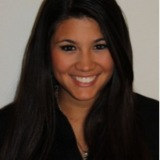
\includegraphics[width=40mm]{images/image011.jpg}
\parbox[b]{0.6\textwidth}{\textbf{Maria Barrera}\\
Status: Mechanical Engineering Graduate Student\\
Contact: mariab8@stanford.edu\\
}

I was born in Colombia and moved to South Florida with my mom when I was 10. My dad and sister still live in Colombia so I tend to hop back and forth every chance I get. I did my undergraduate at Stanford also in Mechanical Engineering and have developed a deep interest for entrepreneurship during my time here. I run a tutoring company in the area and hope to one day start a company in the aviation sector. I also enjoy traveling, photography and playing with puppies.
\\ \\

\noindent 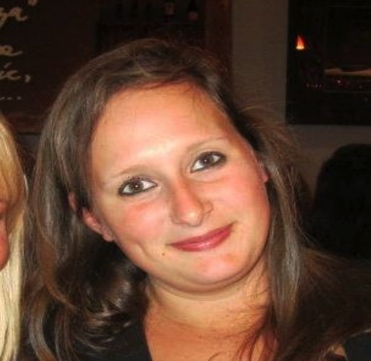
\includegraphics[width=40mm]{images/image012.jpg}
\parbox[b]{0.6\textwidth}{\textbf{Erika Finley}\\
Status: Mechanical Engineering Graduate Student\\
Contact: erikaf@stanford.edu\\
}

I was born and raised in Tennessee. I attended the University of Tennessee at Knoxville for my undergraduate degree in Mechanical Engineering.  I participated in a study abroad in Canberra, Australia.  I have interned for Tennessee Valley Authority at Browns Ferry Nuclear Plant and for Schlumberger at the Rosharon Design Center. I will be interning at Microsoft this upcoming summer. My interests include baking, reading, photography, and roller coasters.  
\\ \\

\noindent 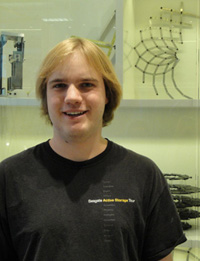
\includegraphics[width=40mm]{images/robert_karol.jpg}
\parbox[b]{0.6\textwidth}{\textbf{Robert Karol}\\
Status: Aeronautics and Astronautics Graduate Student\\
Contact: robkarol@stanford.edu \\
}

I grew up in New Jersey through high school. After that, I moved to southern california where I attended the California Institute of Technology majoring in Mechanical Engineering with minors in Aerospace Engineering and Control and Dynamical Systems. I have worked on robotics projects with NASA's Jet Propulsion Laboratory, as well as experiments in high altitude photography and performed research in microgravity.
\\ \\


\noindent 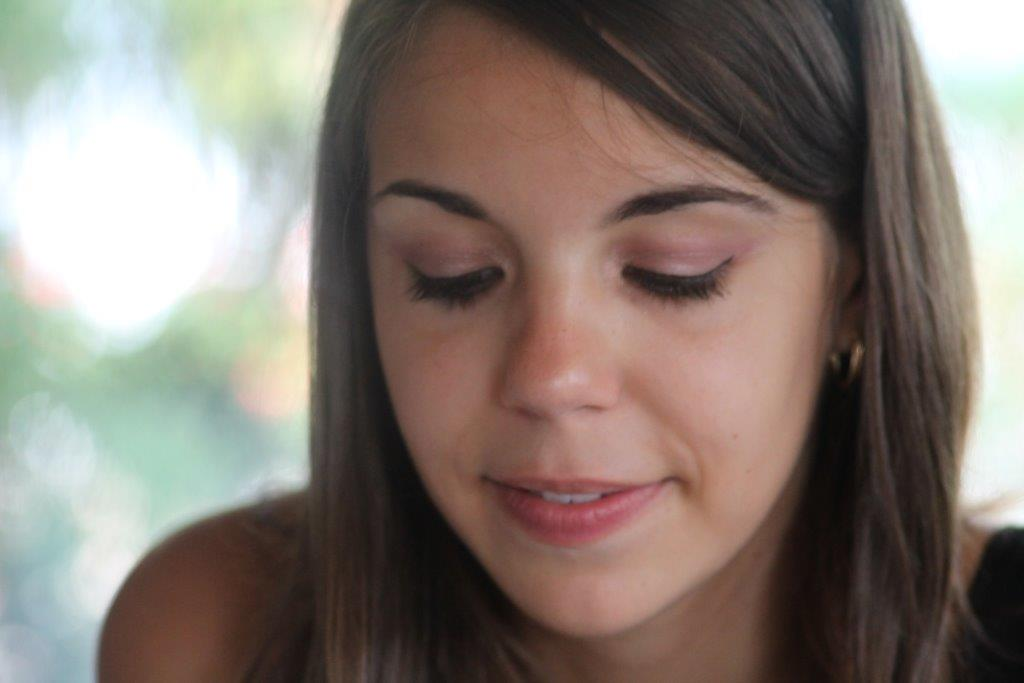
\includegraphics[width=40mm]{images/image012bis}
\parbox[b]{0.6\textwidth}{\textbf{Laura Hoinville}\\
Status: Aeronautics and Astronautics Graduate Student\\
Contact:  laurah31@stanford.edu \\
}

I come from Toulouse, France. I attended ISAE-Supaero (the French Graduate school of Engineering) at Toulouse for my undergraduate degree in Aeronautics. I worked at Airbus head quarters in Blagnac, France as an intern last summer and want to make a career in the field of aircraft design. I'm interested in dance (ballet, modern jazz, contemporary), gymnastics, scuba diving and reading.
\\ \\


\noindent 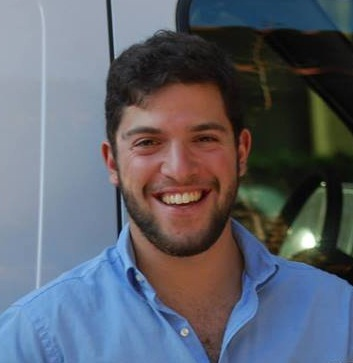
\includegraphics[width=40mm]{images/cliff.jpg}
\parbox[b]{0.6\textwidth}{\textbf{Clifford Bargar}\\
Status: Mechanical Engineering Graduate Student\\
Contact: cbargar@stanford.edu \\
Website: http://cliffbargar.com \\
}

Having spent the first 22 years of my life within a subway ride of Boston, Massachusetts, I decided to drive west and come to Stanford. I'm completing my MSME this spring, focusing on mechatronics, robotics, and controls. I graduated with a BSME from Tufts University, where I double majored in Mechanical Engineering and Mathematics, was an active member of Engineers Without Borders and the Tufts Robotics Club, and ran on the Tufts Cross Country and Track and Field teams. I've spent the last several summers as a student researcher at the Wyss Institute for Bioinspired Engineering at Harvard University, MIT Lincoln Laboratory, and the Tufts Center for Engineering Education and Outreach.

\subsection*{University of S\~{a}o Paulo}

\noindent 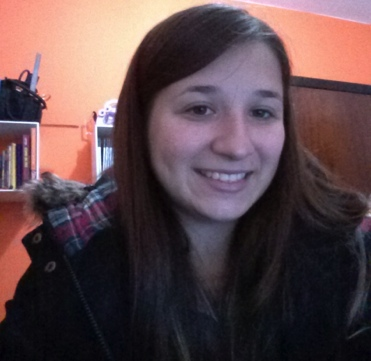
\includegraphics[width=40mm]{images/image013}
\parbox[b]{0.6\textwidth}{\textbf{Amanda Mota Almeida}\\
Status: Product Design Undergraduate Student\\
Contact: amandamotaalmeida@gmail.com \\
}

I was born and raised in S\~{a}o Paulo. I'm attending the University of S\~{a}o Paulo for my undergraduate studies in Product and Graphic Design. I have worked in a project with Embraer in the past regarding the design and comfort in the aircraft cabin (2011), I have interned for Staples in S\~{a}o Paulo – SP (2012) and I was part of exchange in Portugal last year (2013). My interests include: photography, arts and crafts and reading.
\\ \\

\noindent 
\includegraphics[width=40mm]{images/image014}
\parbox[b]{0.6\textwidth}{\textbf{Rodrigo Monteiro de Aquino}\\
Status: Computer Engineering Undergraduate Student \\
Contact: guigonyts@usp.br \\
}

I have lived all my life in S\~{a}o Paulo. I am now graduating in Computer Engineering at USP and I also work in a technology development lab at the university. I have worked on several projects developing educational games and other educational interfaces that help children learn with technological devices.  I like to play videogames and go to the movie theater. I like science fiction movies and reading adventure books.
\\ \\

\noindent 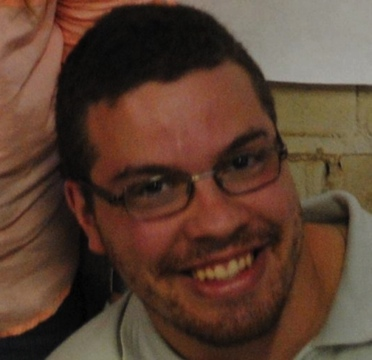
\includegraphics[width=40mm]{images/image015}
\parbox[b]{0.6\textwidth}{\textbf{Luiz Durao}\\
Status: Industrial Engineering Undergraduate Student \\
Contact: luiz.durao@usp.br  \\
}

I was born and raised in S\~{a}o Paulo city. I attended Colégio Etapa for my High School and it was while participating in the Chemistry and Physics Olympiads that I discovered my taste for the sciences. I'm attending the University of S\~{a}o Paulo for my undergraduate studies in Industrial Engineering. I have interned for GE Oil and Gas at Jandira – SP and I have worked since my sophomore year as a teaching assistant for some courses at USP. My interests include soccer, music and movies.
\\ \\

\noindent 
\includegraphics[width=40mm]{images/image016}
\parbox[b]{0.6\textwidth}{\textbf{Guilherme Kok}\\
Status: Industrial Engineering Undergraduate Student \\
Contact:guilhermekok@gmail.com  \\
}

Brazilian and a soccer enthusiast, I grew up in S\~{a}o Paulo and in Baltimore. I've also spent 5 months in Nanaimo (Canada, BC) and 1 year studying at the University of Illinois at Urbana Champaign. I'm currently finishing my undergraduate studies at the University of S\~{a}o Paulo in Brazil, where I study Industrial Engineering. I have interned for a taxi app startup and have done undergrad research concerning the consolidation of the phonographic industry. My interests include playing soccer, hiking, tasting different cuisines and travelling, preferably to remote locations. 
\\

\section{Coaches}

\textbf{Shelly Goldberg} \\
Contact: shelly.goldberg@gmail.com \\ 
Shelly Goldberg was an ME310 alum from 2005, where her team worked on the EADS AugmenTable.  Shelly has been at Apple, Inc. for the past 9 years since leaving Stanford.  She is now a Senior Manager in the Mac Product Design group, where she leads a team of mechanical and product design engineers responsible for conceiving, designing, engineering, producing, and sustaining the Mac portables and desktops.  
\\

\noindent \textbf{Annika Matta} \\
Contact: annikamatta@gmail.com \\
Annika Matta is a former ME310 student and course assistant with a background in product and user experience design. As an ME310er she worked with SAP to build the Nib, a tablet with a writing experience reminiscent of paper. She graduated in 2013 and now works as a user interface designer at a consumer software startup in the Bay Area.
   %Your team, the corporate partner, the project background


%%%%%%%%%%%%%%%%%%%%%%%%%%%%%%%%
% Design Development 
\chapter{Design Development}

Tasked with investigating the future flight experience for disabled passengers, we carried-out process centric and product-centric needfinding and explorations to understand our design space. The insights garnered from these explorations led us to the following key insights which are detailed further in Appendix C.  These insights led us to finally focus on both what happens to the passenger and what happens to his/her wheelchair. The following section is here to show the path our team took to get to this design choice.

\section{User needfinding}
Fall quarter was spent primarily focused on needfinding and benchmarking (see Appendix A) in order to get a firm grasp of the problem we were tasked with solving. Given that ``redesigning the flying experience for people with reduced mobility" is a huge design space with a number of possible users, we used our findings to further develop our understanding of the user segment with the biggest need as well as their specific burning need. After looking at countless available products and interviewing a myriad of different users, we decided to focus on wheelchair users as our target user. 

Throughout our interviews we heard many horror storied about mobility in the cabin and how it affected how wheelchair users prepare for their flights (i.e. ensuring they won't have to use the restroom), how they choose to situate themselves during flight (i.e. choosing to sit in the window seat so they won't be in anyone's way) or how whether they even choose to fly. Our final ``experience" prototype for Fall Quarter involved the idea of having seats on rails that would automatically adjust width when a person needed to enter or exit a row. This way, the wheelchair user would have more room to get into their seat and would also be able to choose the seat they wanted because the row would shift when someone else needed to get out, freeing the wheelchair user of the guilt of being in the way. This design addressed painpoints we all encounter while flying yet would significantly improve the experience for our target user. \\

When we started winter quarter we tried to bring a brand new look and prospectives on the project and in order to get the best out of it we started the quarter by multiple brainstorming sessions in order to identify what were the elements of the aircraft we could change to make the travel experience of the user we deicided to target after the end of fall quarter: a wheelchair user. 

Through these brainstorming sessions we wanted to understand our design space and its limitations. We also wanted to build a strong relationship with our global partners in Brazil and agreed to meet them on Skype at least once a week and share our common work via a Podio web platform. This is how we organized ourselves and tried to tackle the steps of our design development: dark horse and functional prototypes. 

\section{Dark horse}

\subsection{Introduction}
Winter quarter began with the first of three prototyping missions, Dark Horse.  Named for the horse racing term, this prototyping mission fosters the unimaginable and impossible, improbable solutions to the presented problem from Embraer.  The mission called for the brainstorming of out-of-the-box ideas and the  creation of a physical prototype for this plausible solutions.  The learning that occurs from the mission is more important compared to the actual building process due to the intention to guide the team toward their final vision. 

\subsection{Benchmarking}
During our interviews and needfinding research, we realized carry-on luggage was a huge concern. Currently, luggage is stored in a very burdensome and unintuitive way and with our prototype we sought out to redesign the carry-on luggage experience. 
Our users have voiced their concerns about not being able to store/reach their luggage as well as the panic they feel when they are not aware of where their belongings are being stored. Our team looked at a couple of different designs out there that use the vertical space within the airplane in a different manner to accommodate both people and luggage in a more user friendly way. 

\begin{figure}[h]
  \centering
     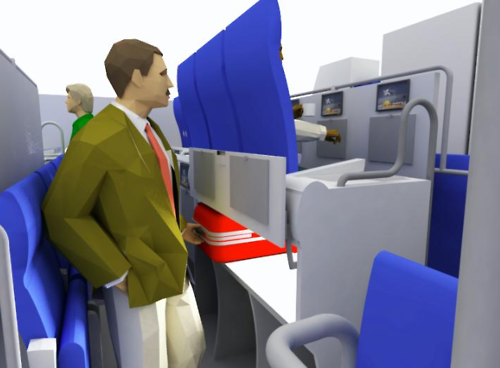
\includegraphics[width=7cm]{images/luggage_trays.png}
   \caption{Design that allows for easier luggage storage for all passengers Source: http://www.gizmag.com/future-of-air-travel-comfortable-seating/17751/}
  \label{fig:luggage_trays.png}
\end{figure}  

The design shown in Figure \ref{fig:luggage_trays.png} displays a cabin layout where consecutive rows of seats are on different levels, allowing passengers to store their luggage behind their tray but under the seat of the person in front of them. This design puts luggage at the ideal height for both standing and sitting passengers as depicted by the image in Figure \ref{fig:correct_height.png}, a standard design rule for access and mobility.  

\begin{figure}[h]
  \centering
     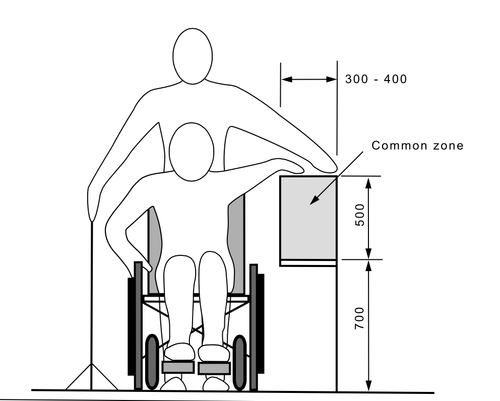
\includegraphics[width=7cm]{images/correct_height.png}
   \caption{Ideal height for reaching objects for both sitting and standing passengers. Source: https://law.resource.org/pub/nz/ibr/nzs.4121.2001.svg.html}
  \label{fig:correct_height.png}
\end{figure} 

Another design solution we explored was actually having two seats on top of each other as shown in Figure \ref{fig:vertical_with_luggage.jpg}. This design opens up the area under the stairs for luggage storage, which could also include a passenger’s wheelchair, allowing for a less stressful flying experience for handicapped users. The bed next to the seat could also be used to provide passengers flying with toddlers with extra room to put them in so that they do not have to sit on their lap throughout the whole flight. 

\begin{figure}[h]
  \centering
     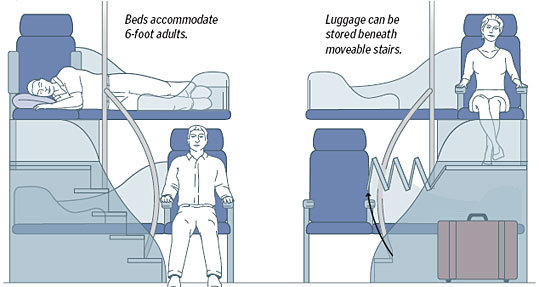
\includegraphics[width=7cm]{images/vertical_with_luggage.jpg}
   \caption{Vertical cabin configuration with luggage storage} % Source: http://www.boston.com/business/articles/2009/06/15/taking_airline_seat_configurations_vertical}
  \label{fig:vertical_with_luggage.jpg}
\end{figure} 


Another main concern for our user was the actual transfer process and how they would get from an aisle chair to their seat. We know that today people can use transfer boards, they can be carried by someone else or, if they are strong enough, they can transfer themselves. We found that there are some products on the market that could make the transfer experience better, such as the “harness” shown in Figure \ref{fig:harness.jpg} or the walker in Figure \ref{fig:walker.jpg}. We believed that the walker would be an interesting solution if we were able to add mechanisms  that would lower the bar supporting the person’s weight to get it closer to the seat and that would swing the blue supports open such that the person would come in contact with the chair. Eventually, we actually decided to widen the airplane aisle and get rid of the transfer all together. 

\begin{figure}[h]
  \centering
     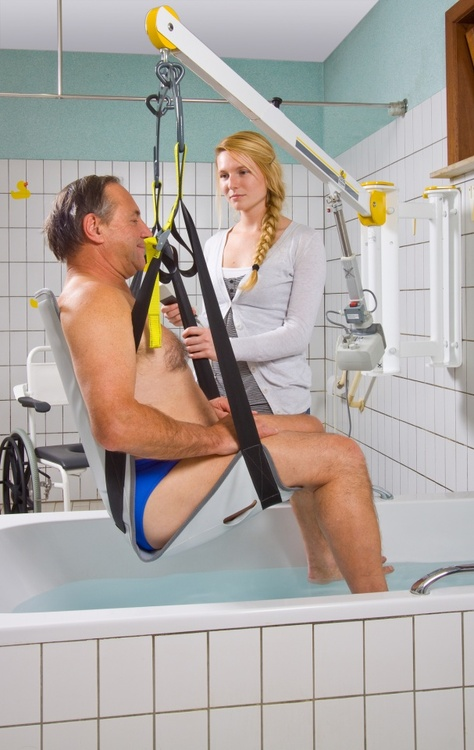
\includegraphics[scale=0.3]{images/harness.jpg}
   \caption{Harness used to get disabled out of the bath.}% Source: http://www.handimove.com/en/products/bath-seat-pvc/}
  \label{fig:harness.jpg}
\end{figure} 


\begin{figure}[h]
  \centering
     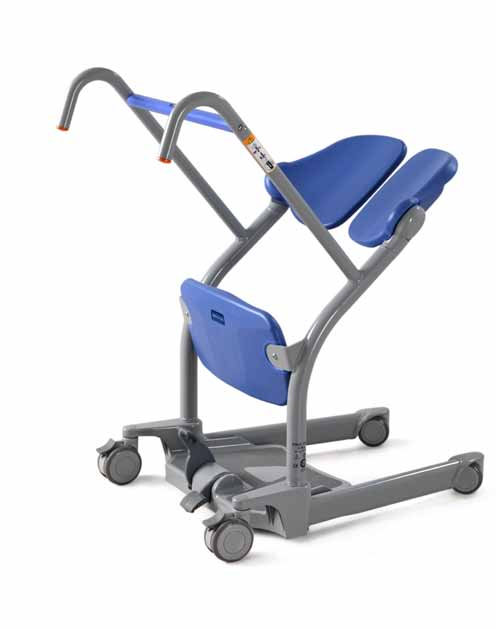
\includegraphics[scale=0.5]{images/walker.jpg}
   \caption{Walker that could be adapted to become a better aisle chair.}% Source: http://mobilityexpress.com/Sara-Stedy-Seated-Transfer-Device_1154.htm}
  \label{fig:walker.jpg}
\end{figure} 

\subsection{Description of the prototype}
Currently, people with reduced mobility have to first transfer from their own wheelchair to the aisle wheelchair which is uncomfortable and narrow. Once boarding starts, the user is brought to his/her seat by a flight attendant or an airline employee and is then transferred to his/her seat. This process is long, it puts people with reduced mobility apart by making them different and it deprives them from their independence because the aisle wheelchair must be manoeuvered by a flight attendant. Therefore, since the boarding process is such a pain point for our users we decided to work on it to improve their experience and give them more independence.

During the boarding process the two steps that are critical for our users are :

 \begin{easylist}[itemize]

& First, the access to their seats. Our team thought that if we could enable people with reduced mobility to enter the aircraft with their own wheelchair and then give them the possibility to transfer themselves from their wheelchair to their seat without someone else helping them it would considerably improve their experience.

& Second, the luggage storage. People with reduced mobility frequently cannot access the luggage compartment because it is too high, so our team thought that if we could imagine a system that makes the luggage compartment go up and down by just pressing a button it would also contribute to make the flight experience better for people with reduced mobility.

\end{easylist}

\newpage

\textbf{1. Helping our user access his/her seat :}

Our objective was to enable passengers to enter the aircraft with their own wheelchair and to do so we had to figure out a way to make the aisle wider. Initially we did not want to take into account the constraint of keeping the number of seats in the aircraft the same so we imagined a new cabin layout for boarding. The idea was to have the aisle seats on rails so that they could be moved and lined up with the window seats as shown in Figure \ref{fig:first_new_cabin_layout} . 

\begin{figure}[h]
  \centering
     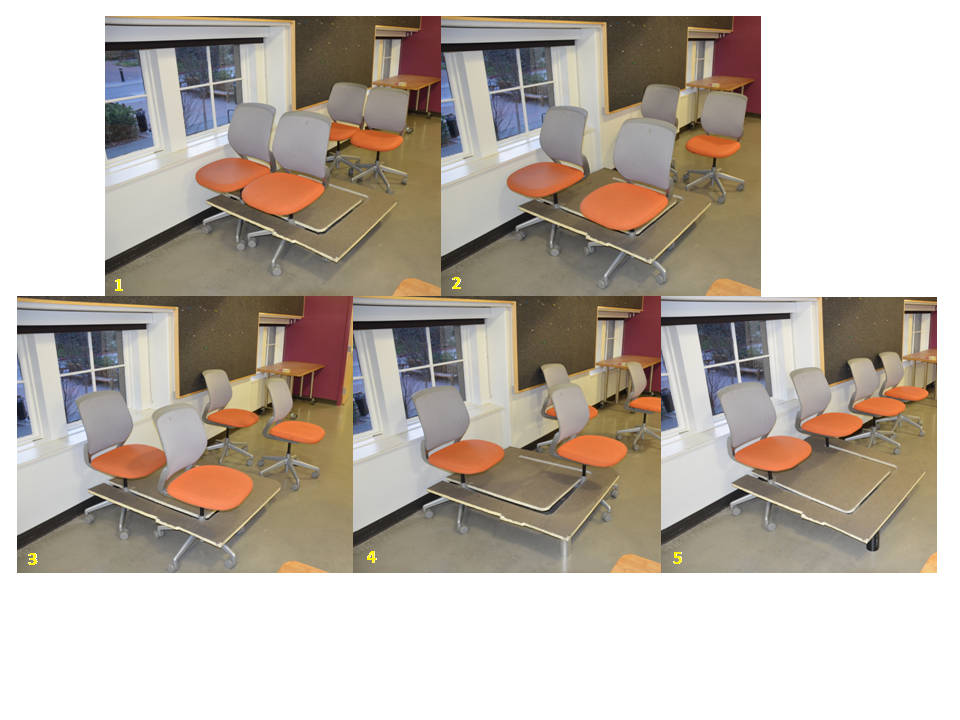
\includegraphics[width=7cm]{images/first_new_cabin_layout.png}
   \caption{Our first new cabin layout for boarding the plane}
  \label{fig:first_new_cabin_layout}
\end{figure} 

With this system all the seats would be lined up on each side of the plane and the aisle during the boarding process would then be three times bigger than in flight, allowing people with reduced mobility to enter the aircraft with their own wheelchair which is on average 30’’ wide, as shown in Figure \ref{fig:wheelchair_dimensions} .

\begin{figure}[h]
  \centering
     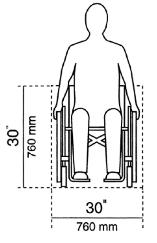
\includegraphics[scale=1]{images/wheelchair_dimensions.png}
   \caption{Standard wheelchair dimensions}
  \label{fig:wheelchair_dimensions}
\end{figure}

But we realized that with this system it was impossible to keep the total number of passengers on board the aircraft the same because the proposed boarding layout requires too much space per seat. 

Therefore, we thought of a second cabin layout for the boarding process which also makes the aisle wider but in a more reasonable way. We looked at the dimensions of a standard Embraer plane (Figure \ref{fig:embraer_plane} ) and found out that if we were able to angle the rows by 46.2° (see Figure \ref{fig:angled_seats}) from their current position we could make the aisle wide enough (42.87’’) to enable our passengers to reach their seats in their own wheelchair while keeping the total number of seats the same.

\begin{figure}[h]
  \centering
     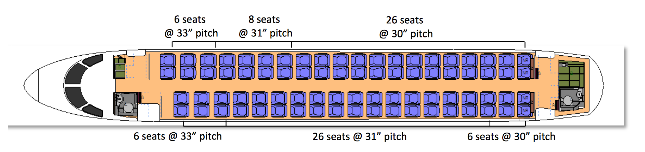
\includegraphics[width=7cm]{images/embraer_plane.png}
   \caption{Standard Embraer plane cabin layout}
  \label{fig:embraer_plane}
\end{figure}

Our concept was to initially have all of the rows of the plane linked to a mechanism that would rotate the seats before the boarding process, making a wider aisle for passengers. Passengers with reduced mobility who have reached their seats with their own wheelchair would be able to transfer to their plane seats. If they are strong enough they may be able to transfer themselves without requesting flight attendants assistance, but if they need help we imagined that they could use one of the transfer mechanisms mentioned in the benchmarking section.
\begin{figure}[h]
  \centering
     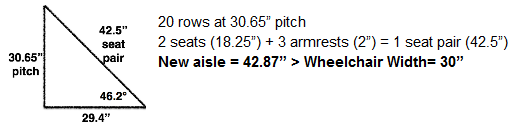
\includegraphics[width=7cm]{images/angled_seats.png}
   \caption{New cabin layout with angled seats for boarding}
  \label{fig:angled_seats}
\end{figure}

Once the passengers are all seated (potentially while the aircraft is taxiing towards the runway) the seats would go back to the standard non angled cabin configuration for take off and would remain in that state for the duration of the flight. When the plane stops at the gate and is ready for passengers to disembark, the seats would be angled again and flight attendants would bring passengers with reduced mobility their own wheelchair so that they would be able to leave the plane on their own.\\ 


\textbf{2. Helping our user accessing the luggage compartment :}

We found out that accessing the seat is not the only problem disabled people are confronted with: they also have a big issue when they want to store their personal items in the luggage compartment. In order to fix this, our team designed a luggage compartment that can go up and down on demand, controlled by our user pressing a button (Figure \ref{fig:embraer_plane}).

\begin{figure}[h]
  \centering
     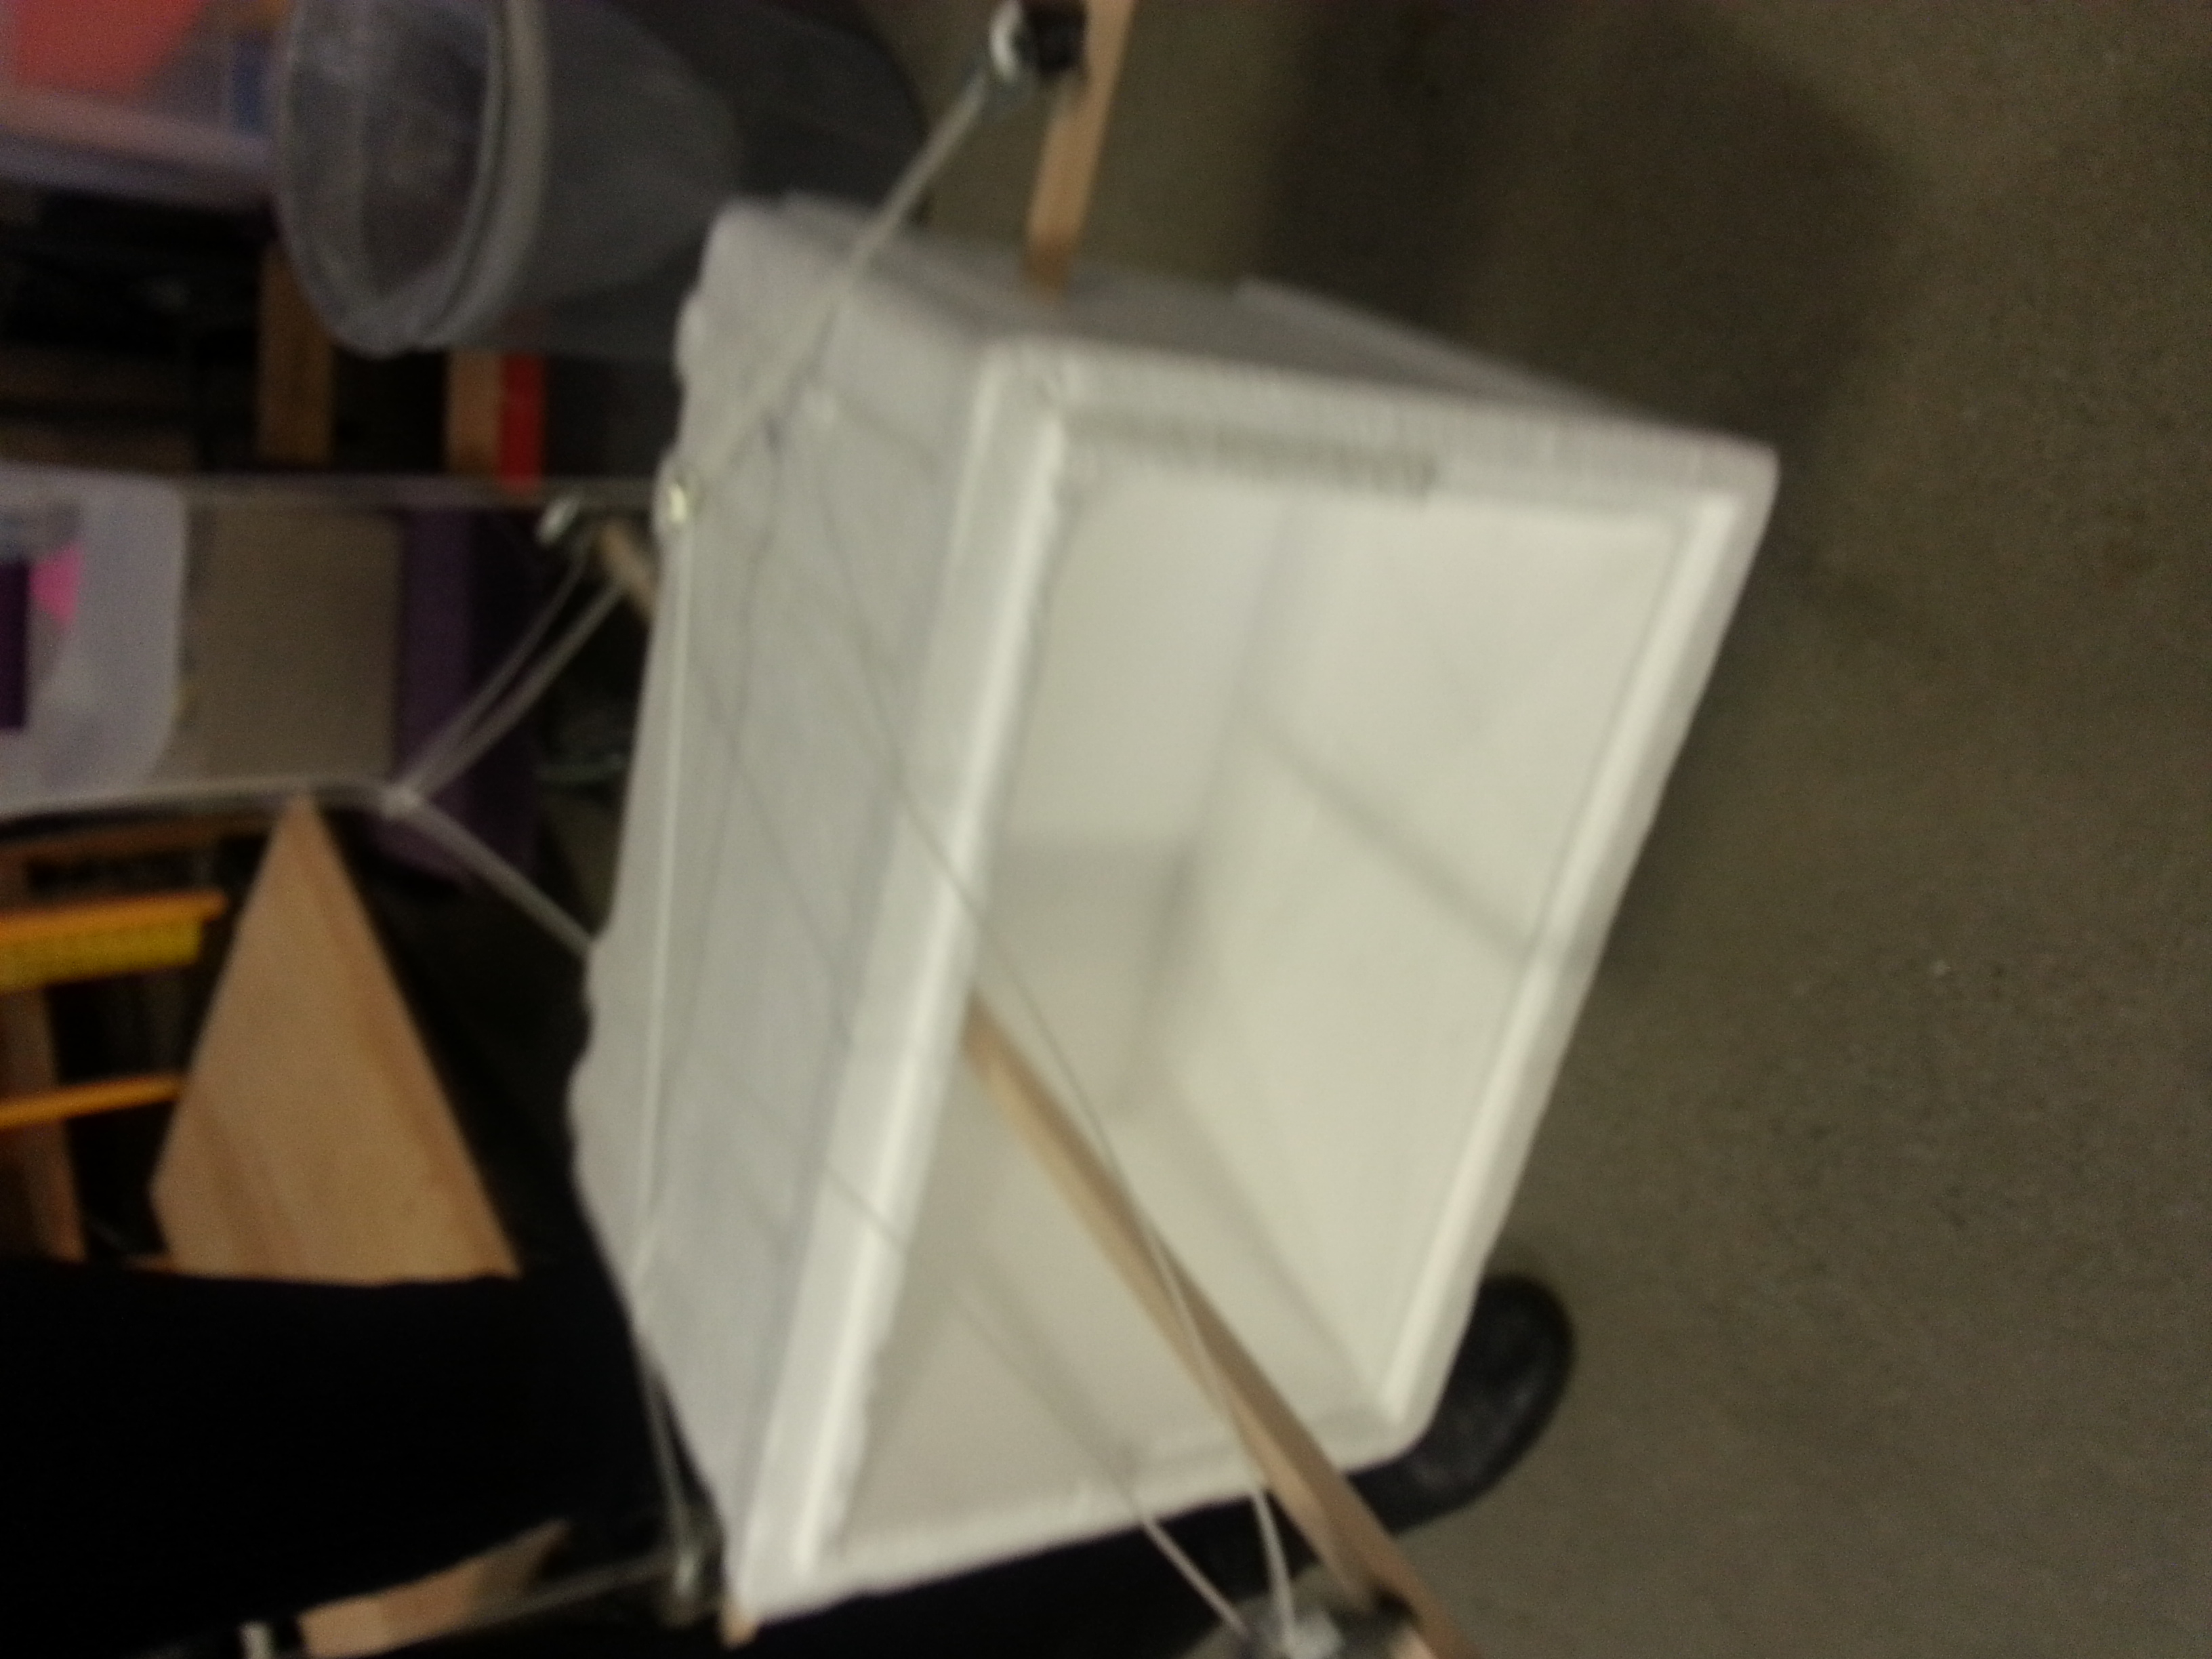
\includegraphics[width=7cm]{images/20140130_170818.jpg}
   \caption{Our luggage compartment which is accessible on demand by pressing a button}
  \label{fig:our_luggage_compartment}
\end{figure}

In order to build this system we designed a mechanism made of rope and pulleys that is inspired from systems used to stabilize cameras that are mounted on drones and model aircraft. While piloting the system that causes the camera to move, the device has to remain stable. This mechanism avoids the creation of moments that could cause the ropes to tangle and knot. For our system we wanted to have a luggage compartment that does not experience torques and that can come up and down in the most smooth and stable way.

\subsection{Learnings}
Several classmates and peers were users for this prototype and provided the majority of our learnings.  However, some of the learnings came directly from team observations during user testing. The learnings are divided into the reconfiguration and the luggage. 

\newpage

\textbf{Reconfiguration:}
\begin{easylist}[itemize]
	& Our testing revealed that the users were concerned about what would happen to their feet during the transformation of angled seating to the regular configuration and vice versa.  Some users suggested the addition of a footrest.  But where would the ideal location be? This revelation is very important to our target users because some of them do not have the ability to move their legs out of the way or to move with the chair.  This would also mean they would have to manually put their feet on a footrest, and the ideal position of the footrest would need to be designed to help the target users have a better experience.
	& A single, continuous rotation mechanism would be better than multiple discrete for all passengers.  The users commented that the mechanism should be similar to the movement of a car seat because it is slow enough and does not cause a great amount of force and acceleration to be placed on the passenger. In addition, the window seat experienced less movement or felt like it experienced less movement than the aisle seat.  This is important due to the benchmarking findings of last quarter that showed that the target users preferred the window seat over the aisle seat. 
	& Passengers would be able to board faster due to a wider aisle that allows for easier maneuvering of the cabin space.  The wider aisle would allow for a double line of traffic to head down the aisle instead of one line. 
	& The wider aisle would allow for a wheelchair to be able to maneuver down the aisle to the seat.  The wheelchair would have tolerances on both sides as it moves down the aisle to allow for a comfortable fit.  It would be easier for a mobility challenged passenger to get into the aisle seat but to access the window a handle may be needed. 
	& The legroom is the limiting factor with the reconfiguration.  When the seats are in the angled arrangement, the window seats have less legroom than in the normal configuration.  The angle of the seats would need to be reconfigured to allow for a smaller angle with more legroom but still create a wider aisle with plenty of tolerance for a wheelchair. However, it was noted that it is easier to board and deboard with angled seats.  Thus, angled seats would be the preferred configuration for boarding and disembarking from the plane. 
	& It may be possible to achieve the desired effect by only rotating several of the aisles, allowing increased access to those seats specifically.

\end{easylist}

\newpage

\textbf{Luggage storage:}
\begin{easylist}[itemize]
	& The luggage bin needs to move with the seats into the angled configurations. With the bins situated parallel to the normal cabin configuration when the seats are angled, it is difficult to load the luggage into the bin without awkward movements. 
	& The luggage bin should be lowered to arm level instead of head or face level.  Users felt claustrophobic when the bin was at head level due to the reduction in vision. The bin was in the line of sight which made it uncomfortable and a very closed-off space.  
	& The bin should have a door and have a slightly steeper angle or have a lip. Luggage moves during flight due to turbulence and shifting due flight. This would prevent luggage falling out on the passengers or items being broken. 
	& A more rigid lowering mechanism needs to be used instead of the string and rope mechanism that was used during prototyping.  Users did not feel that the bin was stable and looked scared as it was lowered down.  They feared the bin might move during lowering, raising, or turbulence causing it to hit them or bring their belongings.  
	& More research for optimal lowering position needs to be conducted.  The position that we prototyped did not receive good feedback from the users.  Therefore, several iterations need to be performed to see what would be best for our target users and other passengers
	& Most of the users wanted to store luggage before they sat in their seat.  The orientation of the bin and the height of the bin makes this a very awkward and uncomfortable task.  When the users sat with their luggage, they felt that they were crowded and did not know what to do with the luggage until the bin was available.  The mechanism to raise and lower the bin needs to be fast and stable to allow for ease of access to the seat and aisle depending on the activity.
\end{easylist}

\section{Going Back to The Need}

Following the wrap up of our prototypes, the team decided to take a step back to figure out if we were truly solving the burning need. We analyzed all of our prototypes up to this point and saw an overarching theme we were trying to address: giving our users their independence back. With independence as our umbrella, our team looked at the whole flying experience piece by piece (see Appendix B), with the purpose of identifying the points at which independence truly breaks down. 

We went back to our needfinding from fall quarter, sent surveys to both old and new contacts and carried out more interviews. All of these allowed us to confirm that mobility within the cabin is, in fact, a huge issue. However, this new information also brought to light a burning need we had initially discarded fall quarter - wheelchair storage. Furthermore, both of these needs stem from the same procedure the wheelchair user is forced to go through: that of giving up his/her wheelchair. \\

\textbf{The Problem}

Imagine you are a wheelchair user. You arrive at your gate, ready to board your plane, and are told you need to hand over your wheelchair for storage in the cargo hold. At this point, you ask yourself two questions: 
\begin{enumerate}
	\item How will you move now that you don't have your mobility device? 
	\item Will your mobility device come back safe and sound at your destination?
\end{enumerate}
The following sections will detail the user quotes and research that led us to choosing both of these directions.  
\\

\textbf{Mobility In the Cabin}

In order to confirm the need for improving mobility inside the cabin, we asked our contacts to fill out a survey that would give us a better idea of what exactly would be the most helpful for them. The full survey responses can be found in Appendix D.
 
When asked about the prospect of having an ``on demand"  powered aisle chair, users were keen on the independence it would provide as it would allow them to ``board the plane at [their] own pace and go to the restroom when [they] please." One of our respondants stated that such a device would allow them to ``feel like a passenger for a change and not a sack of coffee beans". This quote clearly depicts the struggle users currently go through when they give up their mobility device and with it, their independence.

Our team assumed that having such a chair would be a great improvement to the experience yet we could not figure out if the chair had to be completely autonomous and show up on demand or if a flight attendant could bring it to the user. What we found is that users would much rather have automated systems than feel the guilt of inconveniencing someone else to do something for them, even if it only meant they had to bring them a chair just like they bring any passenger a drink or snack. 

Finally, we decided to delve deeper into the transfer process. One of our interviewees, Scott Rains, had told us about a friend who was injured as he was being transferred from the aisle chair into his airplane seat. The airport personnel did not lift him up high enough and his bottom was hit against the armrest. Given that wheelchair users have thinner and more sensitive skin in this area, this caused him lots of pain and even resulted in 3 weeks spent at the hospital. While injuries are not the norm, it is a very dehumanizing and undignified experience, just as Esther Appleyard-Fox states in her tweet in Figure \ref{fig:MobilityTweet.png}. 


\begin{figure}[h]
  \centering
     
\includegraphics[width=9cm]{images/MobilityTweet.png}
   \caption{Tweet from Esther Appleyard-Fox explaining how she feels when she is transferred when she flies. }
  \label{fig:MobilityTweet.png}
\end{figure}


\textbf{Wheelchair Storage}

As we were looking for more data to substantiate our claim that mobility in the cabin was, in fact, the problem to solve, we stumbled upon another huge problem. During our interview with Aubrie Lee, a student in Product Design at Stanford University who is also a wheelchair user, she mentioned that while mobility inside the cabin is a problem, it is such a short part of her experience that she hardly remembers it as being painful. Part of this is due to the fact that when she travels with her dad he carries her down the aisle which I am sure can be more comforting than dehumanizing. However, she emphasized that``the most emotional part of [her] flying experience is having to give up [her] chair and waiting for them to give it back." For her, giving up her chair is ``a huge source of anxiety - as soon as it is out of [her] sight, [she doesn't] know where it is", whether it is going to come back to her unharmed or whether it is even going to make it to her destination. 

In order to understand what can happen to a mobility device on during its transfer to the plane and once in flight, we interviewed an Air France employee working at Toulouse-Balgnac airport (France). All the details form this interview are in Appendix E. It shows how airlines handle wheelchairs from the jetway to the cargo hold and gives some insight on the type of damage that can occur.

A study by Trailblazers \ref{(http://www.mdctrailblazers.org/assets/0000/8262/Trailblazers_AirlineReport_WEB.pdf)}, a group of disabled campaigners across the UK who tackle social issues affecting young disabled people, shows that 60\% of wheelchairs are damaged when traveling with an airline. As David Gillon says in Figure \ref{fig:60percenttweet.png} below, we must do better. 


\begin{figure}[h]
  \centering
     
\includegraphics[width=9cm]{images/60percenttweet.png}
   \caption{Tweet from David Gillon on Trailblazers study that shows 60\% of wheelchairs are broken in airline travel. }
  \label{fig:60percenttweet.png}
\end{figure}

\begin{figure}[h]
  \centering
     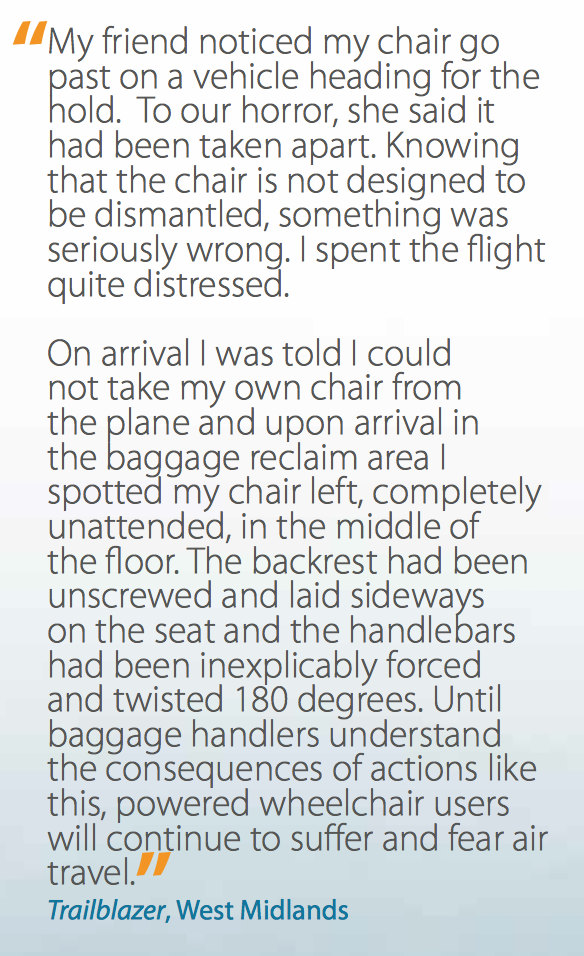
\includegraphics[width=5cm]{images/wheelchairstory.png}
   \caption{Anecdote from a Trailblazer that had her wheelchair broken during flight.}
  \label{fig:wheelchairstory.png}
\end{figure}

Stories like the one shown in Figure \ref{fig:wheelchairstory.png} are not uncommon, with wheelchairs ending up like the one in Figure \ref{fig:brokenwheelchair.png} due to airport personnel attempting to dismantle it or from the wheelchair moving around in the cargo hold. 


\begin{figure}[h]
  \centering
     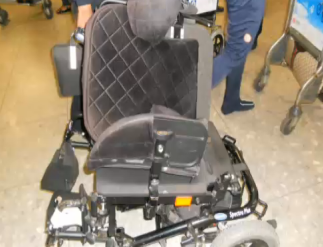
\includegraphics[width=7cm]{images/brokenwheelchair.png}
   \caption{Picture of a broken wheelchair after a flight.}
  \label{fig:brokenwheelchair.png}
\end{figure}

There are also instances of the wheelchair not even making it to the destination, just like what happened to Josie shown in Figure \ref{fig:leftwheelchair.png}. 

\begin{figure}[h]
  \centering
     
\includegraphics[width=9cm]{images/leftwheelchair.png}
   \caption{Tweet from Josie Verguese about her experience when her wheelchair did not make it to her destination.}
  \label{fig:leftwheelchair.png}
\end{figure}

Now to put this into perspective, imagine that you are a wheelchair user and you rely on your mobility device for you independence. This wheelchair isn't just an object, it is your legs, your independence, part of who are you. As Aubrie stated ``it is in limbo between being a physical object and half of me." Now imagine that after your flight, you no longer have the ability to move. This is a HUGE problem for our users, one we need to focus on. \\
\\


 Through  the user interviews, surveys and research depicted above, we have proven to ourselves, our advisors and our users that these are the 2 most compelling needs we need to address for our users and we decided to focus on both for our functional prototype. 


\section{Functional Prototype}
Winter quarter was brought to a finish with the final prototyping mission which desires the creation of a working prototype with system integrations using materials that could be possible in the final vision, which means no duct tape or foam core. The functional mission leads the team into the spring quarter by aiding in the finalization of the vision and creating direction.  To find the direction and the vision, more needfinding might have to take place to confirm a need and verify the thinking and decisions of the team. Functional mission serves as the stepping point from iterative prototyping missions to the iterative final product mission.

\subsection{Wheelchair Storage Benchmarking}
Before prototyping our first wheelchair storage device we did a larger search both for existing wheelchair storage and protection devices as well as methods for securing wheelchairs. We found several relevant patents for protection devices as well as regulations for securement, relating primarily to bus travel. \\

\noindent\textbf{Securement}\\
The United States Department of Transportation's Federal Motor Carrier Safety Administration publishes a wide array of regulations. Included amongst the regulations governing school bus safety, Federal Motor Vehicle Safety Standards \textsection 571.222 \cite{fmvs222}, are a number of requirements for how wheelchairs must be secured while in transit. The section requires that the wheelchair is secured in four locations, with an additional three point mounting required to secure the student. Similar topics are covered in further regulations, such as Title 49 \textsection 38.23 \cite{ecfr}. Figure \ref{fig:tie-down} demonstrates the general setup. \\

\begin{figure}[h]
  \centering
     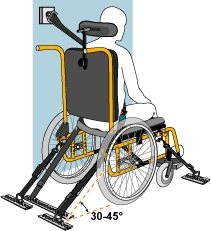
\includegraphics[width=7cm]{images/wc_van.jpg}
   \caption{Wheelchair tie-down setup for van travel}
  \label{fig:tie-down}
\end{figure}

\noindent\textbf{Storage}\\
A group at Utah State University performed market research \cite{USU_survey} and designed a prototype wheelchair storage container, determining that over 50\% of their surveyed users might be or would be interested in their device. A drawing of their box, which provides several securement methods for wheelchairs and other objects, can be seen in Figure \ref{fig:USU_box}; more information is in US Patent application 12/142,662.\cite{USU_patent}

\begin{figure}[h]
  \centering
     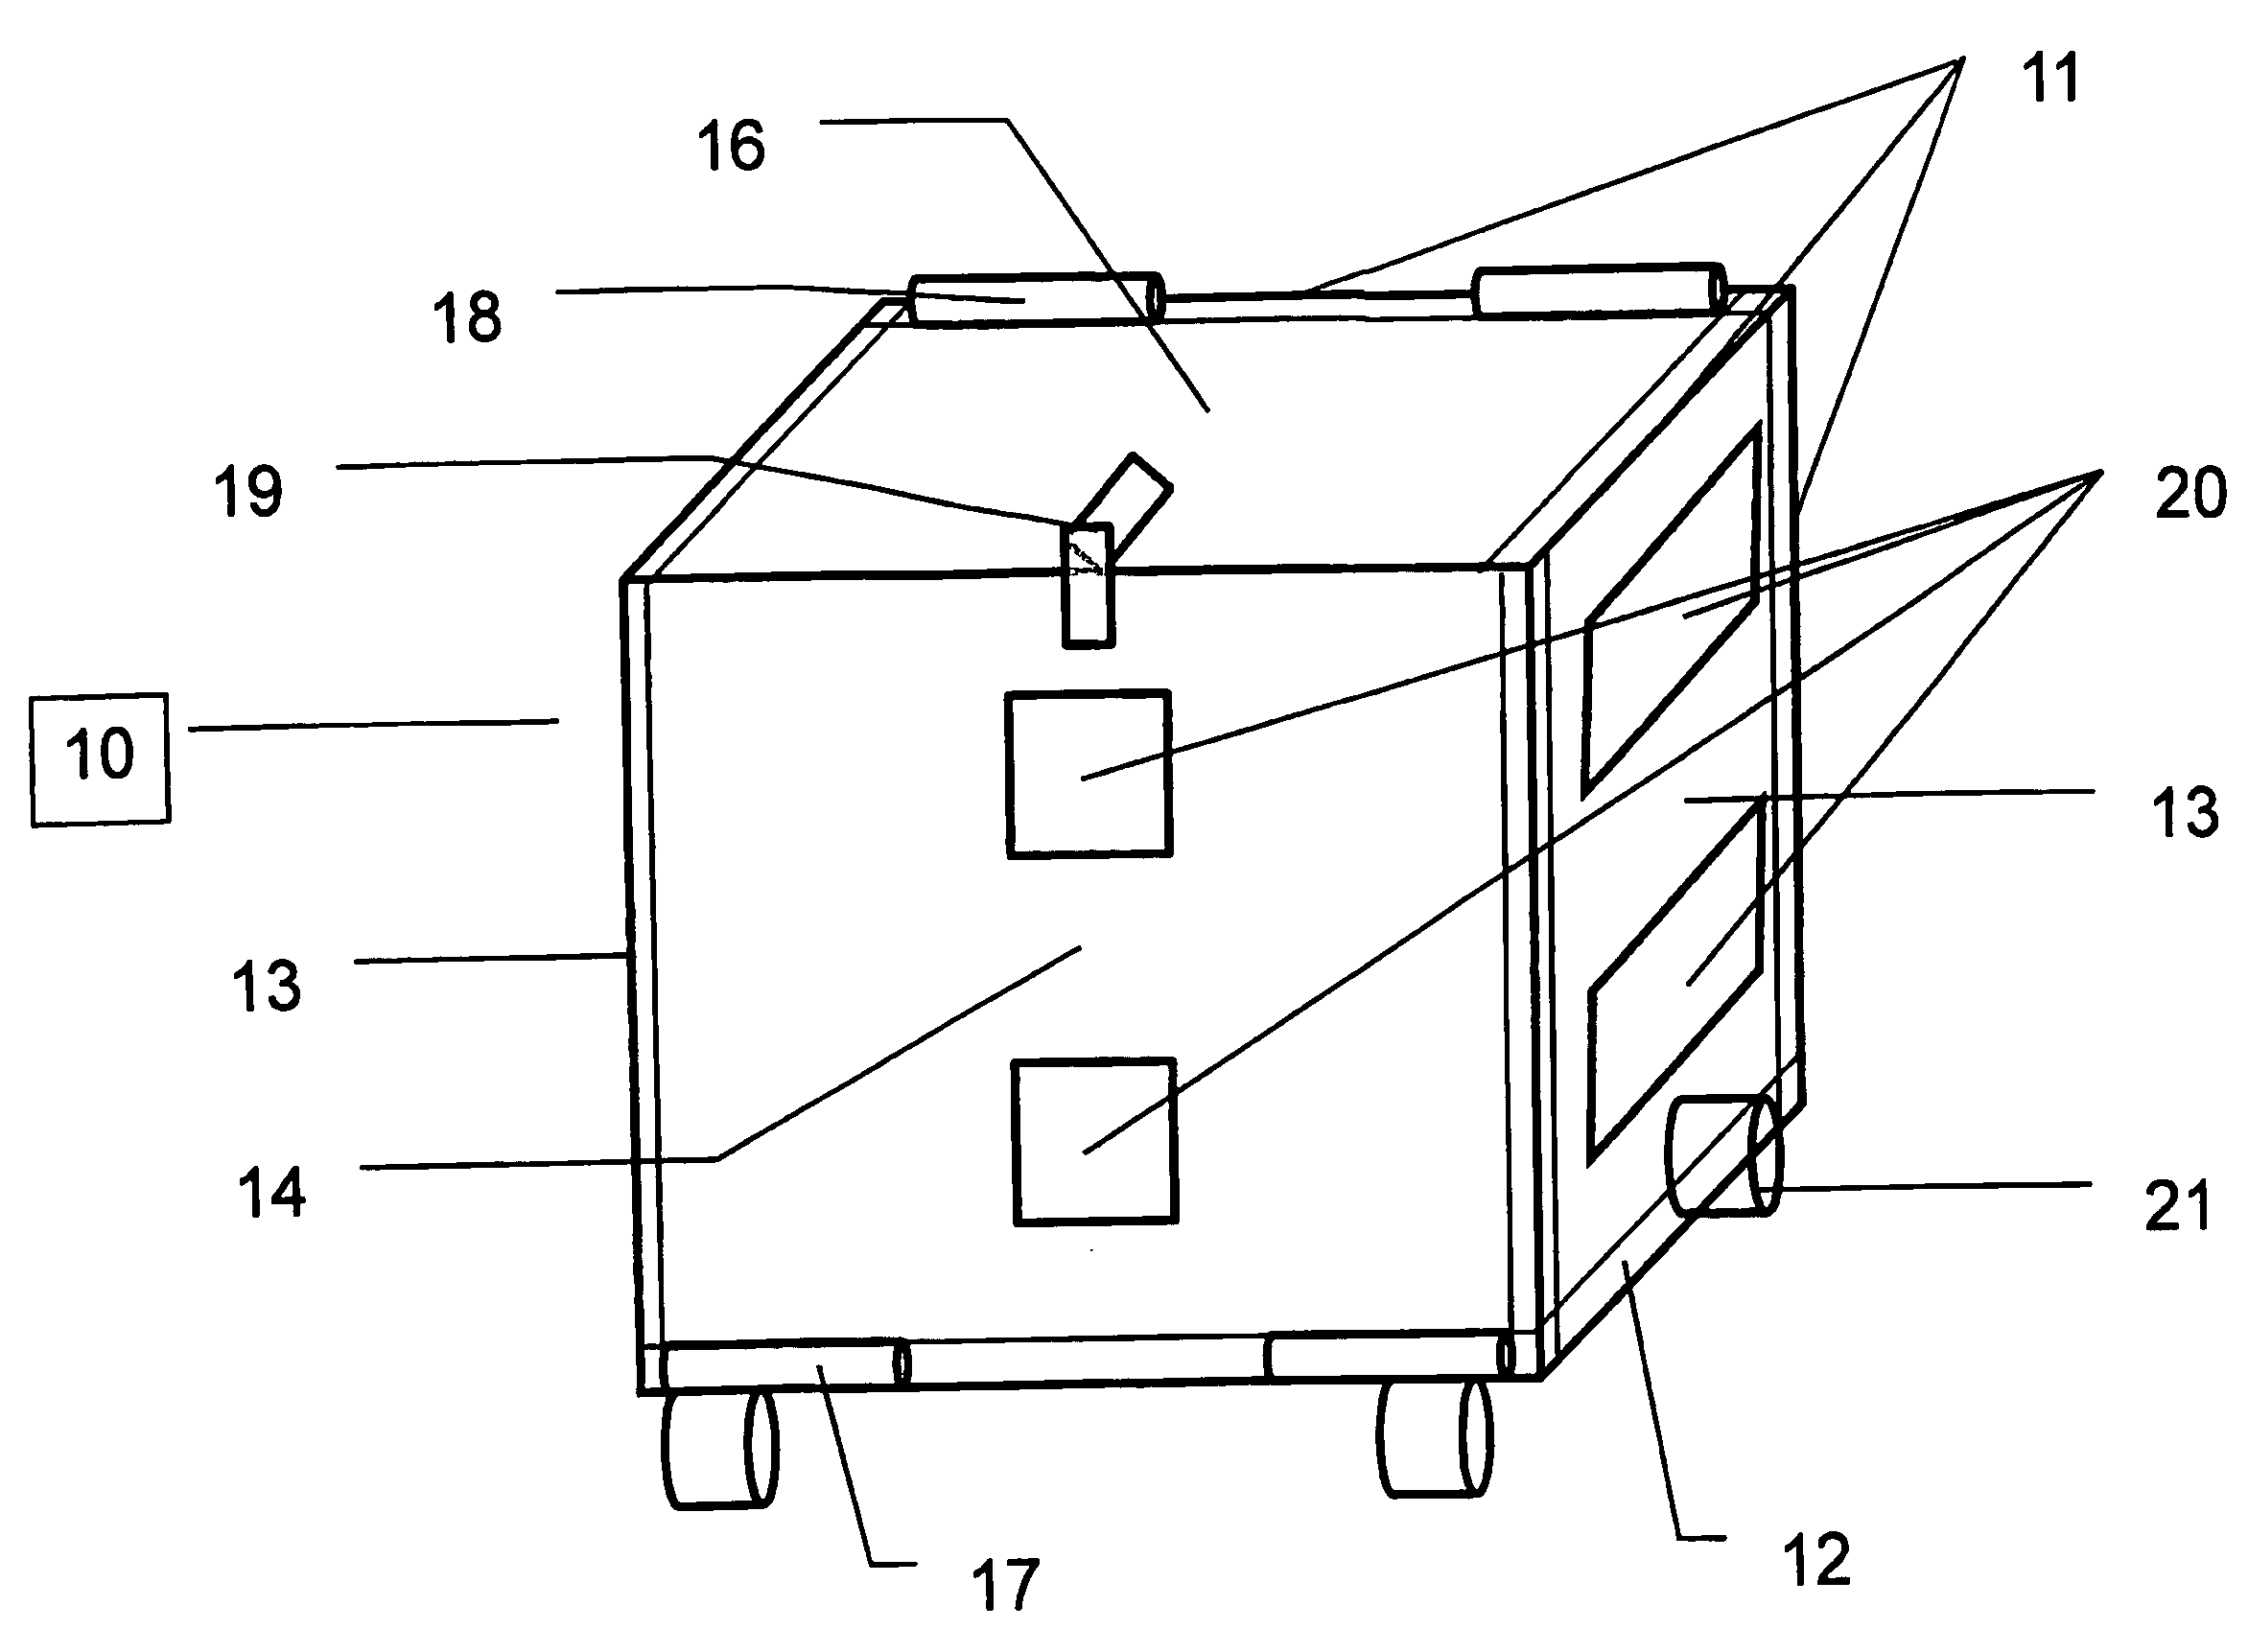
\includegraphics[width=7cm]{images/USU_box.png}
   \caption{Storage container}
  \label{fig:USU_box}
\end{figure}

\newpage

\subsection{Wheelchair Storage Description}

As our last round of needfinding and research had brought to light the importance of wheelchair storage, the Stanford team decided to prototype the first version of what a wheelchair storage device could look like. This first prototype, shown in 
Figure \ref{fig:wheelchairprototype1.png}, focused on having a rigid floor to distribute wheelchair as well as a place to attach the hooks that would secure the wheelchair down. It had rigid walls that would serve to protect the wheelchair (as if it were a box) that were also hinged at the side so they could be moved out of the way of the person tying down the wheelchair. We opted to use the straps and hooks mechanism that people are already familiar with from buses and trains to create a sense of trust an security. 

\begin{figure}[h]
  \centering
     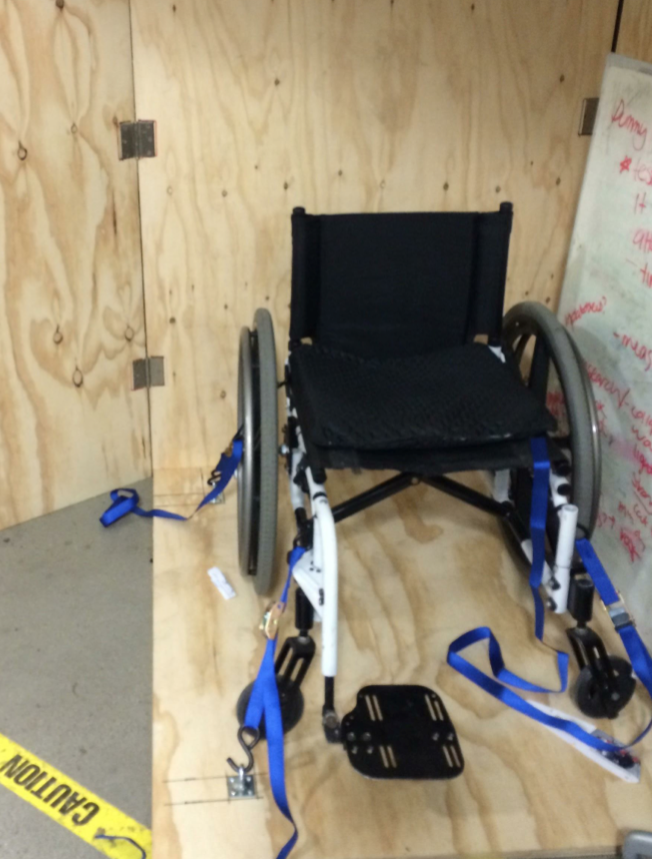
\includegraphics[width=7cm]{images/wheelchairprototype1.png}
   \caption{First prototype of wheelchair storage device.}
  \label{fig:wheelchairprototype1.png}
\end{figure}

Since many of the stories we encountered about wheelchairs being damaged involved airport personnel attempting to disasemble them or handling them poorly, we wanted the wheelchair owner to be present during the securing process, just like they are on a bus or train. This way, the wheelchair user could help the airport personnel speed up the process by providing information about their specific wheelchair and how it should be secured as well as ensure that the airport personnel is not accidentally mishandling their mobility device. At the end of the securing procedure, the container is to be closed up, giving the user feeling satisfaction in knowing that their wheelchair is secure and will arrive safely at their destination. 
 
Part of having the wheelchair user present while their wheelchair is secured is also enabling an easy transfer from their personal wheelchair onto the aisle chair. As shown in the rendering  Figure \ref{fig:storagetransfer.png}, right now this is accomplished by bringing the transferchair close to the passenger's chair that is already secured. This further explains our use of hinged walls and puts a hard constraint on our system- in order for the wheelchair user to be able to easily transfer once their wheelchair is secured, there must be a way to ``remove'' all walls during securing and ``reappear'' them for the wheelchair to be protected.

\begin{figure}[h]
  \centering
     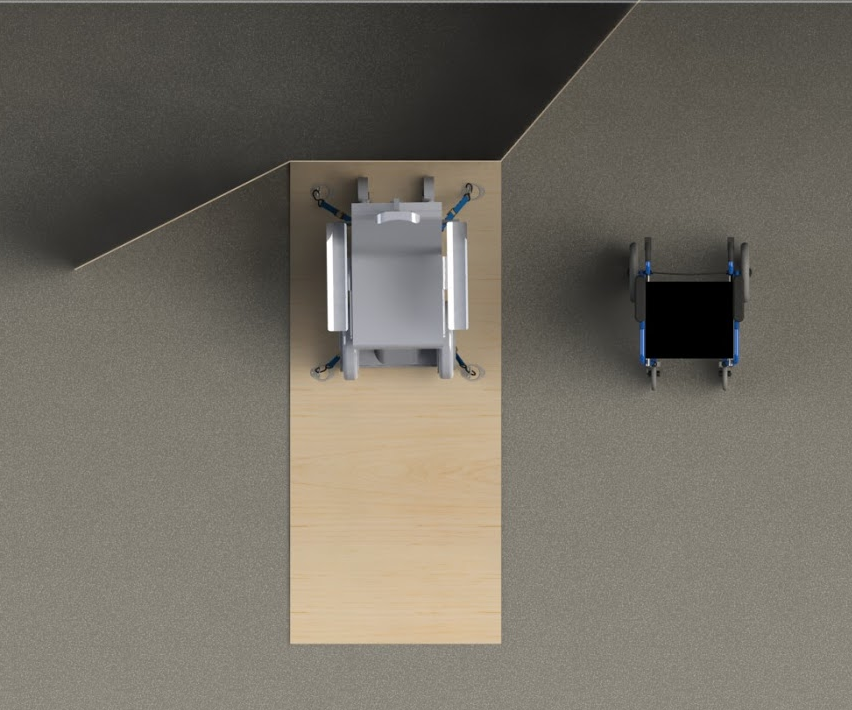
\includegraphics[width=7cm]{images/storagetransfer.png}
   \caption{Rendering of wheelchair and aisle chair side by side once wheelchair has been secured.}
  \label{fig:storagetransfer.png}
\end{figure}

While there are certain hard constraints that were not met with this protoype, we are keeping them in mind and will insitute them in future iterations. We know the container must protect the wheelchair but also fit through the door to the cargo hold as well as fit inside the cargo hold. It needs to be movable, as the wheelchair storage container must travel from the jetway down into the cargo hold. This product must help the luggage handler create a connection with the wheelchair user and gain empathy for the importance of the mobility device that is in their hands; the more important they know it is, the better they will treat it. Finally, the storage device must be lightweight as this is of utmost importance to Embraer.

\subsection{Wheelchair Storage Learnings \& Next Steps}

From our first prototype we were able to learn a myriad of things. Primarily, we realized that using a mechanism that wheelchair users are already familiar with is a huge plus; it provides them with a feeling of trust and security that their wheelchair will not be damaged throughout their flight. Thus, we suceeded at providing the user peace of mind with this device. However, we realized it is pretty difficult to line the chair up in the correctly in between the hook protruding out of the base and thus it would be best to have the hooks be flush against the top of the base so they didn't get in the way of the wheelchair manuevering.
We had several users go through the process of securing the wheelchair and found that having simple straps and hooks can be confusing and time consuming. Thus, it is best to have retractable hooks that come out of the base so that the tension is automatically set, making the job of the securer much easier. 

For a process that takes place prior to a flight, time efficiency is extremely important. Airport personnel are very crunched for time as they cannot afford to have any process delay the flight and push their schedules back. This means having very clear instructions for both the wheelchair user as to what's expectedof them, where to park and how the process will unfold, as well as for the person securing the wheelchair. For the wheelchair user, we are thinking of ways to transfer this imformation prior to their flight, knowing that most disabled passengers keenly do their research before flying. Having a video that shows the whole process would allow the wheelchair user to be prepared to tell the securer exactly what the right attachment points are and how to best secure the wheelchair down. On the other hand, it is important for the securer to know the correct order of the procedure which can be accomplished by numbers next to each hook as shown in Figure \ref{fig:instructionsstorage.png} and simple drawings depicting what's next. 

\begin{figure}[h]
  \centering
     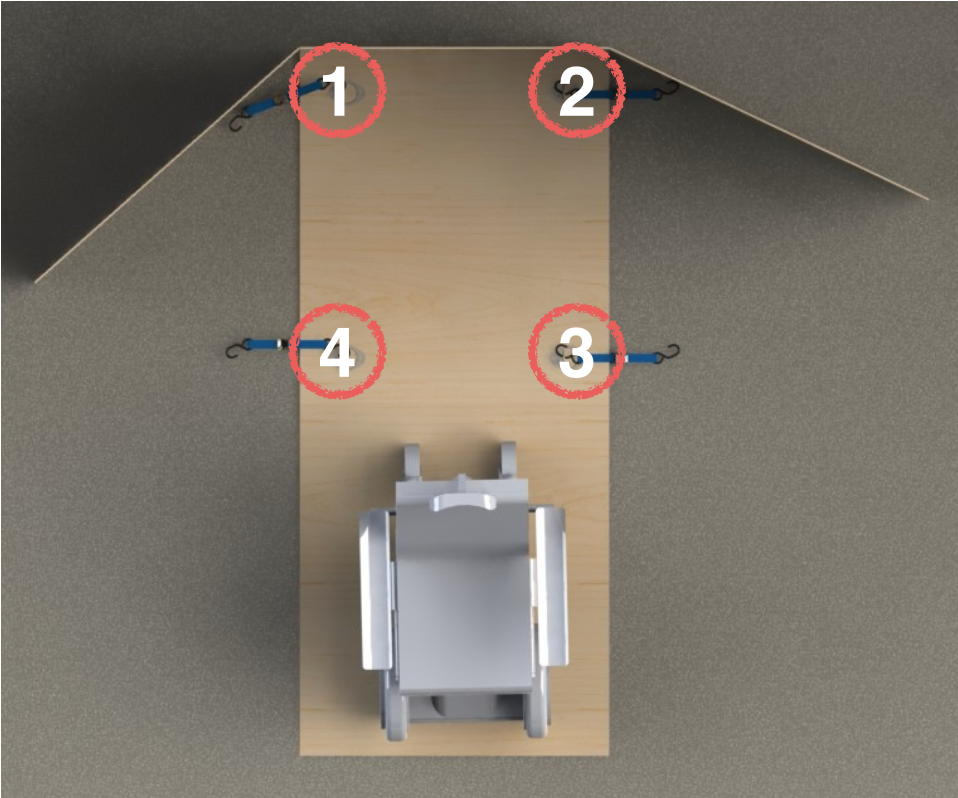
\includegraphics[width=7cm]{images/instructionsstorage.png}
   \caption{Securing the wheelchair}
  \label{fig:instructionsstorage.png}
\end{figure}

Finally, our user testing confirmed our theory that we would need retractable walls. Not only were they necessary for the user to easily transfer onto the aisle chair but they also made the securing process much easier. The back wall, however, was still rigidly attached. This, we found, was not ideal as it made the two hooks in the back extremely hard to reach. With this information in mind, we have been brainstorming different design ideas that would enable for the walls to be completely out of the way during boarding and securing yet would be present during flight to protect the wheelchair from being damaged. We have thought about accordion or telescoping walls as well as having inflatable walls. We really liked the idea of inflatable walls as it provided the wheelchair with protection from damage yet could be blown up to accomodate different types of wheelchair sizes and would be extremely light weight. A preliminary mock up of a possible vision can be seen in Figure \ref{fig:inflatablesrendering.png} With this in mind, we began a feasibility study to understand how possible the use of inflatables would be in the application. 


\begin{figure}[h]
  \centering
     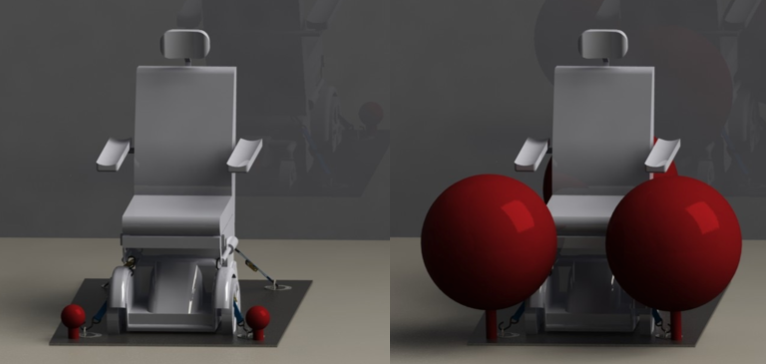
\includegraphics[width=7cm]{images/inflatablesrendering.png}
   \caption{Rendering of a preliminary idea of what an inflatable ``wall'' could be.}
  \label{fig:inflatablesrendering.png}
\end{figure}

%take it from here robbie!

\subsubsection{Inflatable Materials}

In order to test the feasibility of an inflatable device in the cargo hold there were a few problems that needed to be addressed.\\
\noindent\textbf{Pressure}\\
The cargo hold of many planes is not pressurized in order to save on costs. One of our goals was to determine if an inflatable device to protect the wheelchair would pose a problem in low pressure situations. Initially we were unsure as to what the pressure in the cargo hold would be, and as such decided to design for the worst case when the pressure is the same inside the cargo hold as outside. 

It was important to design for this case as regardless of the pressure in the cargo hold, in any emergency situations where the cabin lost power, we would not problems to arise in the cargo hold potentially making the situation worse.\\

\noindent\textbf{Temperature}\\
A second potential problem with an inflatable device in the cargo hold is that the luggage does not require the same heating and insulation as passengers. While it may not get as cold as the air outside (approximately -40 C) in normal situations, as in the pressure situation the device must be designed reliably for an emergency. \\

\noindent\textbf{Testing}\\
While it may be possible to test the effects of pressure on an inflatable device without taking it into a plane by increasing the pressure inside the inflatable device since the pressure differential is the most important aspect to test. However, its much more difficult to test this pressure differential at a realistic temperature on the ground. Instead we decided it would be best to get an inflatable structure up to approximately the height of a plane and determine what failure modes if any would be present. 

In order to do this we attached an arm flotation device fully filled to a weather balloon. This balloon was released in order to take the device into the upper atmosphere where it would experience similar conditions to those of an airplane. While it ignores some effects from the natural plane insulation, its a more extreme environment in all cases so its a good measure of feasibility. \\

\noindent\textbf{Results}\\
Unfortunately the barometer which was being used as an altimeter for this experiment failed, and as such we were unable to get reliable altitude data on the flight. However by looking at the videos returned from the launch, and given the groups prior experience with weather balloons a reasonably reliable estimate of 50,000 - 60,000 ft can be estimated for when the flotation device popped which is significantly higher than an embraer jet flies (37,000 ft maximum). We were able to see small water droplets on the larger weather balloon which froze at altitude forming ice crystals.


\subsubsection{Wheelchair Tracking Concept}

We envision a wheelchair tracking system in which each storage container has a unique identifier, such as a QR code, which can be tracked as the container moves from the jetway to the tarmac, into the cargo hold, and then back out again after landing. The identifier can be recognized at a series of checkpoints, which need only consist of a webcam if a QR code is used. Such a system will provide our users with the peace of mind that their mobility device has not been mistreated or left behind.

\begin{figure}[h!]
  \centering
     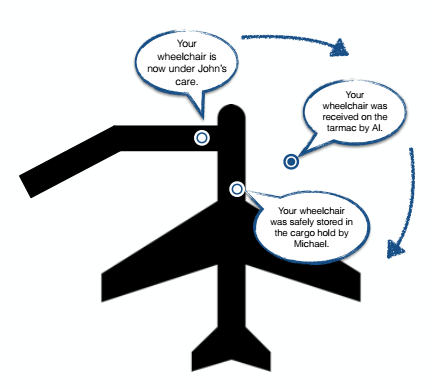
\includegraphics[width=12cm]{images/tracking.png}
   \caption{Wheelchair tracking system overview.}
  \label{fig:tracking}
\end{figure}

\newpage

An important aspect of this system is that it can also help develop empathy on the part of the baggage handlers. Wheelchair users will have the opportunity to tip handlers who've done a good job in managing their mobility device, both providing an incentive for doing a better job while also helping form a closer connection between two people who may never meet face to face.

An overview of the system and one potential user interaction are in Figures \ref{fig:tracking} and \ref{fig:tips}.


\begin{figure}[h]
  \centering
     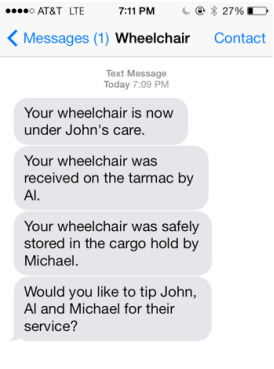
\includegraphics[width=7cm]{images/tips.png}
   \caption{One possible minimal interface for user interaction with the tracking system.}
  \label{fig:tips}
\end{figure}

\newpage

\subsection{Transfer mechanism from aisle wheelchair to seat}

Once the problem of wheelchair storage storage is addressed, there is still one that needs to be solve: how do disabled passengers reach their seats once their mobility device is stored in the cargo hold? line of thought: how can we make the access easier inside the airplane to people with reduced mobility? \\

Our benchmark and interviews showed us that the transfer is one of the most demeaning moments for the handicapped, so the team focused on making the user more independent while transferring. \\

\subsubsection{Candidates}
The team agreed that the prototype should make the transfers inside the airplane so easy that the person on the aisle wheelchair could make the transfer by himself without major efforts. After a brainstorm, the team had two ideas for making this transfer: a sliding seat and a comb mechanism in which a male/female coupling system would allow the user to be transferred. The former mechanism was chosen because it was simpler to build and lighter, as it did not require a motor to lift the user or a counterweight to stabilize the chair. With that in mind, we benchmarked existing mechanisms that were used to make linear transfers. These mechanisms are listed below: \\

\noindent\emph{Linear Guide}\\
The rails would be installed on the aisle wheelchair and the seat, while the carriage would be installed on the cushion. The cushion would be able to slide from one seat to the other if the seat and the wheelchair were correctly paired.

\begin{figure}[h]
\centering
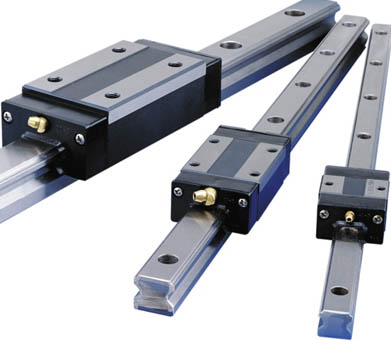
\includegraphics[width=7cm]{brazil_images/image035.jpg}
\caption{Linear guide} % - http://www.yesillerrulman.com/staf_lsk_ome_lineer_kizakli_araba_ray.html}
\label{fig:linear_guide}
\end{figure}

The negative aspect of the linear guide is that it would require a milimetric precision when pairing the aisle wheelchair with the seat. We found this to be unrealistic, especially when we took in consideration that the solution would not necessarily be automated.\\

\noindent\emph{Conveyor rollers}\\
The mechanism would use the same principles of a conveyor table, where one can move heavy objects by sliding them on top of conveyor rollers. This mechanism would be installed on the seat and the aisle wheelchair, allowing the cushion with the user to slide.

\begin{figure}[h]
\centering
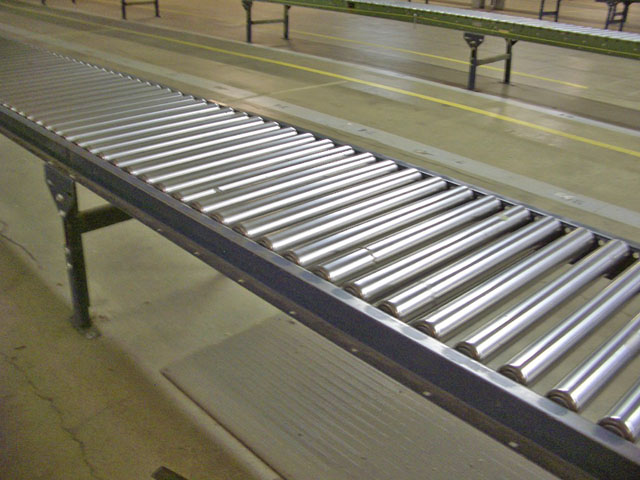
\includegraphics[width=7cm]{brazil_images/image036.jpg}
\caption{Conveyor rollers} % - http://qdtmzdhsb.cn.gongchang.com/product/d27215965.html}
\label{fig:conveyor_rollers}
\end{figure}

\newpage

\noindent\emph{Ball transfer table}\\
The mechanism would work as the previous one, where the cushion would be able to slide from the aisle wheelchair to the seat, but using spheres instead of conveyor rollers. These spheres are lighter than the previous solution and as a result were more appropriate for our design.

\begin{figure}[h]
\centering
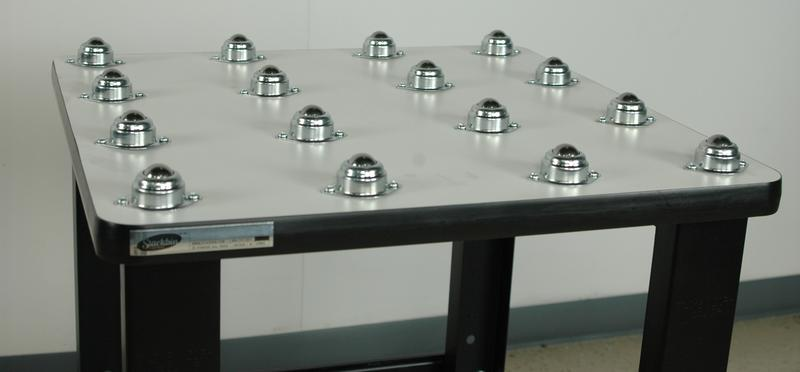
\includegraphics[width=7cm]{brazil_images/image037.jpg}
\caption{Ball transfer table}% -  http://www.stackbin.com/categories/ball-transfer-tables/ }
\label{fig:ball_transfer}
\end{figure}

Unfortunately, for our first prototype, we could not find a supplier that could provide the components in time to build the prototype with an affordable cost, so the mechanism with conveyor roller was chosen. For the final prototype, the team was finally able to get this device and implement it.

Based on what was discussed above, for the first version, the team decided to implement the seat with conveyor rollers to enable the sliding movement of the seat (Figure \ref{fig:idea_mechanism}). With the same mechanism installed on the aisle wheelchair, one would be able to easily transfer oneself laterally from the aisle wheelchair to the seat and vice versa without major efforts.

\begin{figure}[h]
\centering
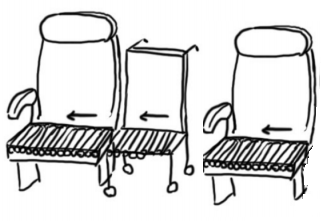
\includegraphics[width=7cm]{brazil_images/image038.png}
\caption{Idea of the mechanism}
\label{fig:idea_mechanism}
\end{figure}


\subsubsection{Building our prototype}
In our first attempt to build the prototype (Figure \ref{fig:first_attempt}) the high friction made the sliding movement extremely difficult. The main reason for this failure was that our initial assumption that the aluminum cylinder directly attached to the wooden structure would be enough to make the rolling movement was false. \\

\begin{figure}[h]
\centering
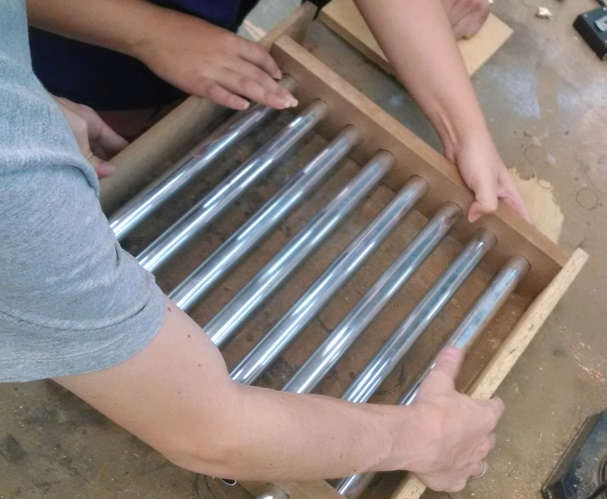
\includegraphics[width=7cm]{brazil_images/image039.jpg}
\caption{First building attempt}
\label{fig:first_attempt}
\end{figure}


In order to overcome this issue, we added bearing to both ends of the cylinders (Figure \ref{fig:fixing_bearings}). This solved the friction problem, making the whole mechanism work as we had designed it (Figure \ref{fig:final_mechanism}).	


\begin{figure}[h]
\centering
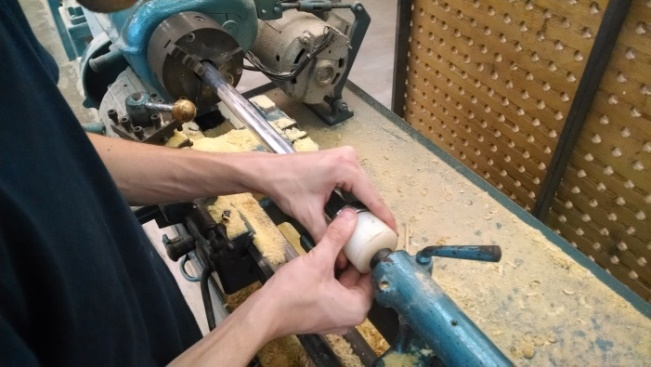
\includegraphics[width=7cm]{brazil_images/image040.jpg}
\caption{Fixing bearings}
\label{fig:fixing_bearings}
\end{figure}


\begin{figure}[h]
\centering
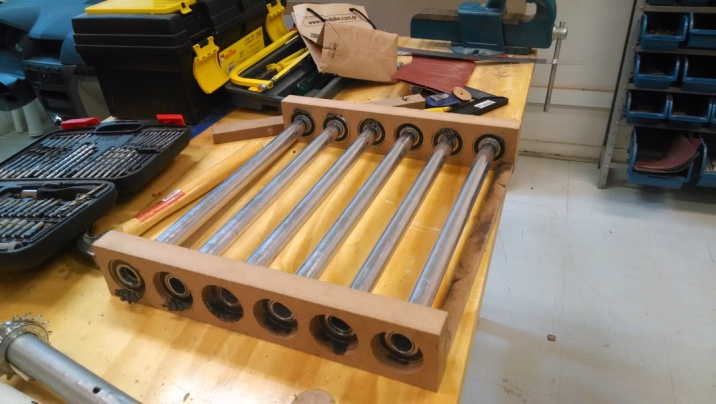
\includegraphics[width=7cm]{brazil_images/image042.jpg}
\caption{Final mechanism}
\label{fig:final_mechanism}
\end{figure}

Next, we tested the sliding mechanism with different types of materials on the cushions base. First we tried adding an adherent surface (rubber) to see how the mechanism would slide. We noticed that it was quite hard to overcome the static friction. Afterwards we tried adding a semi-rigid plastic base. Although the transfer was quite easy, one could feel the cylinders while sliding. As a result, we chose to use a hard flat base under the cushion to make it slide smoothly.   \\


\subsubsection{Learnings}

\begin{itemize}
	\item The friction between the aluminum cylinder and the wood is too intense for a user to transfer from one seat to another
	\item The space between the cushion and the mechanism must be considered to avoid at the same time increasing the friction and the looseness of the cushion (rotating movement)
	\item Cushion must be firm enough so that the user does not feel the cylinders and to allow proper transfer
	\item Correct alignment between the aisle chair and the seat is very important.
	\item Armrest must be retractable.
	\item It is possible, quite easy and comfortable to make a lateral transfer.
	\item Understanding how the mechanism will be used is crucial for achieving a user-friendly design. For instance, by simulating how a transfer would be made by an user, we noticed that it made sense to link the latching mechanism with the movement of the armrest. Armrest up, seat unlocked and vice-versa. We had several options for locking the seat, but we insisted in finding one that would be intuitive for the user. This proved to be a good design choice.
	\item Our conveyor rolling mechanism is not viable because it required too many alterations of the airplane and added too much 
\end{itemize}

\section{Our vision for the final product}

From all the prototypes our team built during winter quarter we decided to combine the two products: the wheelchair platform and the transfer mechanism into one single enhanced experience for passengers with reduced mobility. \\

Figure \ref{fig:our_vision} shows the different steps our user should go through in order to get a much better flying experience than what they have today. \\


\begin{figure}[h]
  \centering
     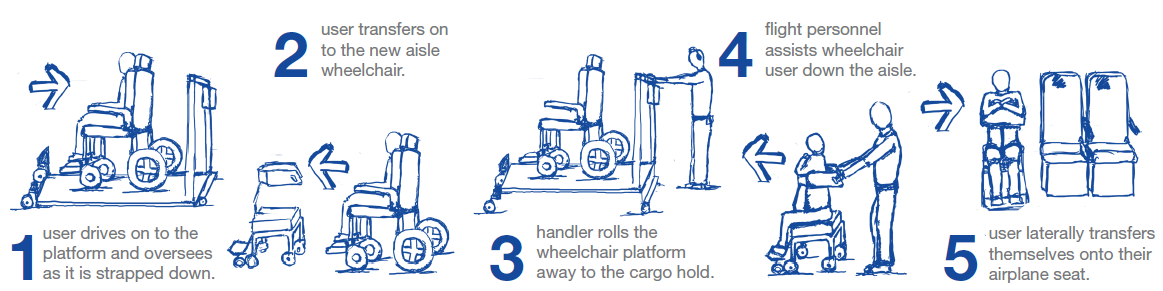
\includegraphics[width=16cm]{images/our_vision.png}
   \caption{Our vision for the final product}
  \label{fig:our_vision}
\end{figure}

In order to include the two products (wheelchair platform and transfer mechanism) into the one single experience for the passengers, we realized that our team would also have to redesign completely the aisle wheelchair to enable a smooth transfer from the passenger’s wheelchair to the airplane seat.\\

\newpage

With this vision in mind, our objective for the spring quarter was to build and test with users:
\begin{itemize}
\item The wheelchair platform
\item The redesigned aisle wheelchair
\item The transfer mechanism integrated into an airplane seat
\end{itemize}

All the design requirements associated with these products are presented in the next section and the design specification section gives many details about the design solutions we implemented for each system.\\

Unfortunately, due to time constraints, we did not get th opportunity to develop and create a smartphone app that would provide wheelchair users with information about their trip and the way their mobility device is handled by the airline. We instead decided to focus more on the hardware than the software but additional information about the app can be found in Appendix G.

  .

% Design Requirements
\chapter{Design Requirements}

The following requirements are based on the problem statement, team brainstorming, user needfinding, and prototypes described in the design development section. Some of this requirements also come from a geometrical and structural analysis of the plane (cabin and cargo hold) that are detailed in Appendix F.
\\
\\This requirements fall into two categories: Functional and Physical. Functional requirements detail what a design should do, its actions and capabilities. Physical requirements describe the constraints on the manifested system components. 
\\
\\ We have divided the functional and physical requirements into two main parts:
\begin{list}{-}{}
  \item Requirements for the wheelchair platform that will improve wheelchair storage from the jetway to the cargo hold
  \item Requirements for the transfer mechanism that will enable wheelchair passengers to reach their seats in a more comfortable and independent way
\end{list} 

\section{Functional Requirements}

\subsection*{Wheelchair storage device}

In order to prevent wheelchairs from being damaged our team wants to design a platform that will enable baggage handlers to move the mobility device from the jetway to the cargo hold. This platform will be composed of five parts:

\begin{list}{-}{}
  \item A pallet that will support the wheelchair
  \item A moving mechanism to enable transport from jetway to cargo hold
  \item Electronics that will identify who is handling the wheelchair and detect mishandling
  \item A handle that will enable baggage handlers to interact with the platform
  \item A ramp that will enable the wheelchair to be driven on top of the pallet
\end{list}

The functional requirements for each of this part are in the tables from \ref{fig:fun_req_pallet} to \ref{fig:fun_req_ramp}.

\newpage

\begin{figure}[h!]
  \centering
     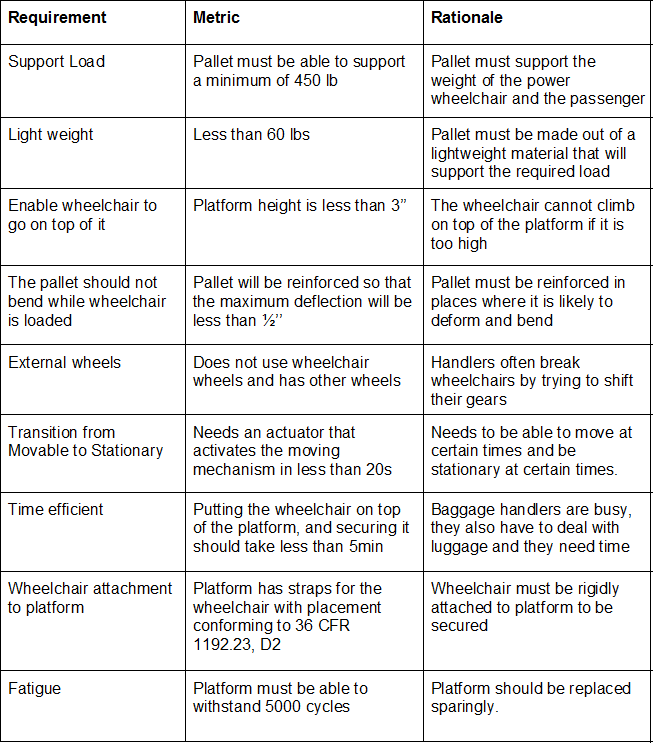
\includegraphics[scale=1]{images/functional_requirements_pallet.png}
   \caption{Functional requirements for the pallet}
  \label{fig:fun_req_pallet}
\end{figure}

\newpage

\begin{figure}[h!]
  \centering
     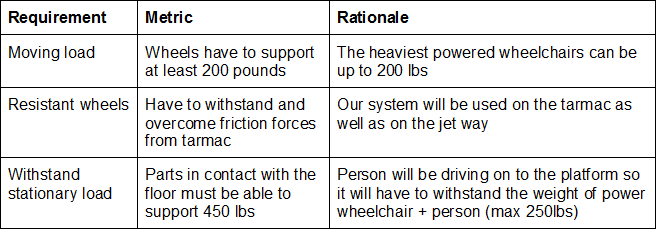
\includegraphics[scale=1]{images/functional_requirements_moving_mechanism.png}
   \caption{Functional requirements for the moving mechanism}
  \label{fig:fun_req_moving_mechanism}
\end{figure}

\newpage

\begin{figure}[h!]
  \centering
     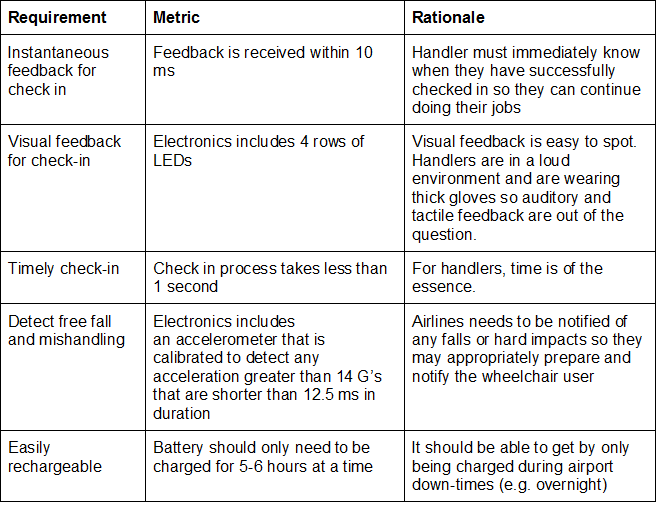
\includegraphics[scale=1]{images/functional_requirements_electronics.png}
   \caption{Functional requirements for the electronics}
  \label{fig:fun_req_electronics}
\end{figure}

\newpage

\begin{figure}[h!]
  \centering
     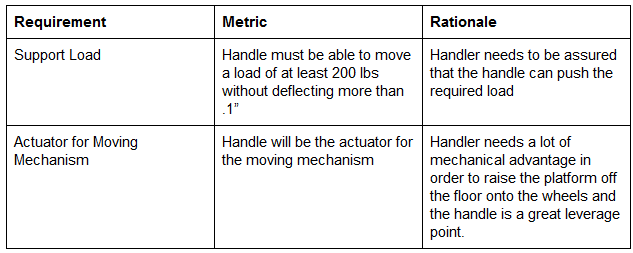
\includegraphics[scale=1]{images/functional_requirements_handle.png}
   \caption{Functional requirements for the handle}
  \label{fig:fun_req_handle}
\end{figure}

\newpage

\begin{figure}[h!]
  \centering
     \includegraphics[scale=1]{images/functional_requirements_ramp.png}
   \caption{Functional requirements for the ramp}
  \label{fig:fun_req_ramp}
\end{figure}

\newpage

\subsection*{Wheelchair transfer mechanism}

In order to improve the boarding experience for disabled passengers, our team decided to redesign the aisle wheelchair by making it possible for a wheelchair user to transfer himself from the wheelchair to his seat without needing to be carried by flight attendants. The system that we are designing to give wheelchair users their independence back will be composed of seven parts:

\begin{list}{-}{}
  \item A chest rest that will equip the aisle wheelchair in order to make its use more comfortable and less degrading for passengers
  \item A locomotion mechanism that would enable wheelchair users to move through the cabin
  \item A cushion that will support disabled passengers
  \item A sliding base that will enable transfer from the aisle wheelchair to the airplane seat without external assistance
  \item A wheelchair structure that will completely be redesigned to accomodate the sliding base and the chest rest
  \item A footrest that will enable disabled passengers to have support for their legs
  \item A new airplane seat that will be adapted to the sliding base
\end{list}

The functional requirements for each of this part are in the tables from \ref{fig:fun_req_chest_rest} to \ref{fig:fun_req_airplane_seat}.

\newpage

\begin{figure}[h!]
  \centering
     \includegraphics[scale=1]{images/functional_requirements_chest_rest.png}
   \caption{Functional requirements for the chest rest}
  \label{fig:fun_req_chest_rest}
\end{figure}

\newpage

\begin{figure}[h!]
  \centering
     \includegraphics[scale=1]{images/functional_requirements_locomotion_mechanism.png}
   \caption{Functional requirements for the locomotion mechanism}
  \label{fig:fun_req_locomotion_mechanism}
\end{figure}

\newpage

\begin{figure}[h!]
  \centering
     \includegraphics[scale=1]{images/functional_requirements_cushion.png}
   \caption{Functional requirements for the cushion}
  \label{fig:fun_req_cushion}
\end{figure}

\newpage

\begin{figure}[h!]
  \centering
     \includegraphics[scale=1]{images/functional_requirements_sliding_base.png}
   \caption{Functional requirements for the sliding base}
  \label{fig:fun_req_sliding_base}
\end{figure}

\newpage

\begin{figure}[h!]
  \centering
     \includegraphics[scale=1]{images/functional_requirements_wheelchair_structure.png}
   \caption{Functional requirements for the wheelchair structure}
  \label{fig:fun_req_wheelchair_structure}
\end{figure}

\newpage

\begin{figure}[h!]
  \centering
     \includegraphics[scale=1]{images/functional_requirements_footrest.png}
   \caption{Functional requirements for the footrest}
  \label{fig:fun_req_footrest}
\end{figure}

\newpage

\begin{figure}[h!]
  \centering
     \includegraphics[scale=1]{images/functional_requirements_airplane_seat.png}
   \caption{Functional requirements for the airplane seat}
  \label{fig:fun_req_airplane_seat}
\end{figure}

\newpage

\subsection{Functional Constraints}

\subsection*{Wheelchair storage device}

\begin{list}{-}{}
  \item Due to FAA regulations and flight requirements the platform protecting the wheelchair must withstand 3 G's.
  \item The platfrom cannot damage the space or items within the space during its operation.
  \item The electronics will require a power source (battery) to perform some of its functions.
  \item The battery should satisfy the DOT’s Hazardous Materials Regulations (HMR; 49 CFR parts 100-185).
  \item The entire device needs to be approved as safe for air travel.
\end{list}

\subsection*{Wheelchair transfer mechanism}

\begin{list}{-}{}
  \item Due to FAA regulations and flight requirements every element that goes inside the cabin must withstand 6 G's.
  \item The redesigned aisle wheelchair must be as safe as the standard aisle wheelchair operated nowadays.
  \item The new aisle wheelchair has to operate in the restrained space of the airplane aisle.
  \item In case of turbulences, the wheels of the new aisle wheelchair must be blocked.
\end{list}

\subsection{Functional Assumptions}

\subsection*{Wheelchair storage device}

\begin{list}{-}{}
  \item Since the straps that are used to attach the wheelchair to the platform are the same as bus straps, wheelchair users are assumed to already be familiar with them. The use of this mechanism should provide them peace of mind since they already trust it in buses.
  \item The platform configuration changes (on the wheels to be moved or on the pallet to be stored) will be trigered by baggage handlers acting on an electric jack.
  \item Baggage handlers will be wearing their gloves with the RFID tag everytime that they handle a wheelchair and use our platform.
\end{list}

\subsection*{Wheelchair transfer mechanism}

\begin{list}{-}{}
  \item All aisle seats must have retractable armrest. It must allow the mechanism to slide without any obstacles in its way.
  \item The passenger will always be accompanied by a flight attendant to guarantee the safety of the passenger and to pull/push the aisle wheelchair.
  \item Tetraplegic passengers will always be accompanied by a travel companion/assistant. Because of regulation (ANAC) and their reduced autonomy, tetraplegic users are not allowed to fly alone.
  \item The airplane seat must withstand 19 G's during take-off and landing. This is what the FAA requires in order to make sure seats can withstand any type of accident happening during take-off or landing.
\end{list}

\subsection{Functional Opportunities}

\subsection*{Wheelchair storage device}

\begin{list}{-}{}
  \item Our platform must be intuitive to use. A baggage handler should know how to attach a wheelchair to the platform after a 15 mn training.
  \item Ideally the platform should have a braking system for the wheels to prevent it from moving too fast on a sloped surface. A braking device would allow handlers to have better control on the device.
\end{list}

\subsection*{Wheelchair transfer mechanism}

\begin{list}{-}{}
  \item Although we are desiging for a paraplegic user, it shall allow a tetraplegic user to be transferred from the aisle wheelchair to his/her seat with assistance. In this case, it should be a more pleasant experience since the assistant would not need to lift the tetraplegic user.
  \item The chest rest makes frontal transfer possible. Nowadays it cannot be done due to the current wheelchair dimensions.
  \item It reduces the risk associated to transfer because no one is carrying the disabled passenger. The chest rest is here to avoid human contacts that can be unpleasant and/or source of accidents.
  \item The chest rest allows paraplegic passengers to go to the restroom and use it.
\end{list}

\newpage

\section{Physical Requirements}

\subsection*{Wheelchair storage device}

\begin{figure}[h!]
  \centering
     \includegraphics[scale=1]{images/physical_requirements_pallet.png}
   \caption{Physical requirements for the pallet}
  \label{fig:phy_req_pallet}
\end{figure}

\newpage

\begin{figure}[h!]
  \centering
     \includegraphics[scale=1]{images/physical_requirements_electronics.png}
   \caption{Physical requirements for the electronics}
  \label{fig:phy_req_electronics}
\end{figure}

\newpage

\begin{figure}[h!]
  \centering
     \includegraphics[scale=1]{images/physical_requirements_handle.png}
   \caption{Physical requirements for the handle}
  \label{fig:phy_req_handle}
\end{figure}

\newpage

\begin{figure}[h!]
  \centering
     \includegraphics[scale=1]{images/physical_requirements_ramp.png}
   \caption{Physical requirements for the ramp}
  \label{fig:phy_req_ramp}
\end{figure}

\newpage

\subsection*{Wheelchair transfer mechanism}

\begin{figure}[h!]
  \centering
     \includegraphics[scale=1]{images/physical_requirements_chest_rest.png}
   \caption{Physicall requirements for the chest rest}
  \label{fig:phy_req_chest_rest}
\end{figure}

\begin{figure}[h!]
  \centering
     \includegraphics[scale=1]{images/physical_requirements_locomotion_mechanism.png}
   \caption{Physical requirements for the locomotion mechanism}
  \label{fig:phy_req_locomotion_mechanism}
\end{figure}

\begin{figure}[h!]
  \centering
     \includegraphics[scale=1]{images/physical_requirements_cushion.png}
   \caption{Physical requirements for the cushion}
  \label{fig:phy_req_cushion}
\end{figure}

\begin{figure}[h!]
  \centering
     \includegraphics[scale=1]{images/physical_requirements_sliding_base.png}
   \caption{Physical requirements for the sliding base}
  \label{fig:phy_req_sliding_base}
\end{figure}

\newpage

\subsection{Physical Constraints}

\subsection*{Wheelchair storage device}

\begin{list}{-}{}
  \item The wheelchair load (more than 600 lbs for the heaviest wheelchairs) must be distributed over a minimum surface area of 8 in2 otherwise the stress experienced by the cargo hold floor will be too high and the floor may collapse. (All the details explaining how we got the 8 in2 figure are shown in appendix F).
  \item For th RFID identification system, the distance between the antenna and the tag must be as small as possible. The outer plastic surface covering the RFID antenna must be less than .25''.
  \item The box that encloses all the electronics must be very light weight (less than 3 oz).
  \item Power wheelchairs cannot climb an angle steeper than 6 degrees so the must inclination must be below this metric.
\end{list}

\subsection*{Wheelchair transfer mechanism}

\begin{list}{-}{}
  \item The width of the aisle (19.75'' in Embraer jets E175) limits the size of the aisle wheelchair.
  \item The new aisle wheelchair must be less than or equal to current aisle wheelchairs which weigh approximately 35 lbs.
\end{list}

\subsection{Physical Assumptions}

\subsection*{Wheelchair storage device}

\begin{list}{-}{}
  \item The ramp has to be modular. It is an attachment, not the platform itself because wheelchairs shoud not be stored at a 6 degree angle during a long flight. 
  \item The ramp has to be removed once used otherwise it would take too much space in the cargo hold.
\end{list}

\subsection*{Wheelchair transfer mechanism}

\begin{list}{-}{}
  \item We assume that the average wheelchair passenger using our transfer mechanism will have an average weight of 180 lbs.
  \item If disabled passengers have the opportunity to use the new redesigned aisle wheelchair to go to the restroom, we assume that this restroom is accessible and must have lateral grab bars.
\end{list}

\newpage

\subsection{Physical Opportunities}

\subsection*{Wheelchair storage device}

\begin{list}{-}{}
  \item The handle that enables baggage handlers to move the platform should be ergonomic. They should be covered by an ergonomic sleeve made of material such as silicon in order to increase comfort of pushing the platform around.
  \item The ramp should be attached to the platform in order to reduce the number of parts the airport personnel needs to handle.
  \item Having a hinged ramp serves double purpose. It can be used as a ramp and also as a stopper in case the wheelchair unstraps. It is here to increase user's peace of mind.
\end{list}

\subsection*{Wheelchair transfer mechanism}

\begin{list}{-}{}
  \item Wheelchair transfer from the passenger's wheelchair to the new aisle wheelchair will happen once the passenger has driven his/her mobility device on top of the platform. This way, baggage handlers do not manipulate the wheelchair at all. They only touch the platform. This should provide piece of mind to our user.
  \item Wheelchair users that are overweight should feel more comfortable in our redesigned aisle wheelchair because there is more support on the side.
\end{list}

   

% Design Specifications
\chapter{Design Description}

\section{Wheelchair Storage}

\subsection{The platform}

As explained in the design requirements, our platform had to be able to support the weight of a very heavy power wheelchair while at the same time being as lightweight as possible. For this reason, we decided to make the main parts of our platform out of aluminum. In the future, we can imagine a platform constructed out of composite material that would increase the strength and decrease the weight. However, for our proof of concept, aluminum turned out to be a great material choice. 
 
Indeed, this material is very resistant, it has a yield stress of 240 MPa and it is very light with a density of 2.7 g/cm3. In terms of feasibility, it was also relatively easy to find the aluminum we needed at a reasonable price. We purchased a 0.125in thick flat plate of aluminum with the following dimensions- 36’’x50’’. These dimensions are slightly larger than what is considered to be the minimum amount of area for securing a wheelchair according Federal Motor Vehicle Safety Standard 222. We also ordered 80/20 made to create the structure, reinforce the main frame and make the handle of the platform.
 
\begin{figure}[h]
\centering
\includegraphics[width=9cm]{images/platform1.jpg}
\caption{The platform we designed using aluminum}
\label{fig:platform1}
\end{figure}
 
As we were analyzing and simulating the effects of the wheelchair load with ANSYS, we realized we needed to add a frame under the aluminum plate because the flat plate would bend if the load applied exceeded 300lbs. As shown in figure \ref{fig:platform2} the ANSYS analysis which was carried out for a 400 pound load applied at four contact points (each one simulating a wheel) shows a lot of bending. The maximum deflection in this case was 2.6 inches, a deflection that is no longer negligible.
 
\begin{figure}[h]
\centering
\includegraphics[width=10cm]{images/platform2.png}
\caption{ANSYS analysis of the platform aluminum plate}
\label{fig:platform2}
\end{figure}
 
For this reason, we chose to increase the stiffness of the plate by adding an 80/20 bar along the sides of the platform and three additional 80/20 bars in the middle. This was enough to decrease the bending of the aluminum and did not add much weight (roughly 20 pounds)
 
Because we needed to raise and lower the platform (see moving mechanism section for more details), we decided to add extra stiffness on the edges by adding an aluminum angled bar on each side as shown in figure \ref{fig:platform3}.
 
\begin{figure}[h]
\centering
\includegraphics[width=7cm]{images/platform3.jpg}
\caption{The angled bar and the straps we added to the platform}
\label{fig:platform3}
\end{figure}
 
Figure \ref{fig:platform3} also shows another feature we added to the main part of the platform: the straps. As explained previously, we needed to secure the wheelchair once it was on top of the platform. We decided to use straps found in public transportation today because our users are already familiar with them and they trust them. We did not add any other protection device because through our needfinding we were able to infer that wheelchairs mainly get damaged when travelling from the jet way to the cargo hold. Indeed, wheelchairs are the last item put inside the cargo hold and the first one taken out, so it is unlike that baggage handlers throw bags on top of it and airline employees generally use nets inside the cargo hold to make sure heavy items remain static. For this reason, we chose to only use the straps to tie down the wheelchair and did not add other protection device. We could imagine that a next version of our prototype could have inflatable or other material to protect the wheelchair. 
 
The last main feature of the platform is the handle. As you can see from Figure \ref{fig:platform1}, we made it out of the aluminum 80/20. We designed it such that baggage handlers were pushing the platform and not pulling it since this would enable them to look at the wheelchair while moving the whole system. To determine the optimal height of the handle our team did some research on ergonomics of dollies and pallet jack. We found out that according to the Center for Occupational Health and Safety the ideal height was 44 inches from the ground as shown in Figure \ref{fig:platform4}. This is the appropriate placement for an average adult who is 5 feet 8 inches  to use his/her arms to push something heavy while minimizing the effort required to do so. In the future, we could improve the ergonomics of this handle by adding a silicon sleeve to the section that is in contact with handlers’ hands, giving them further information on where exactly they should push and providing them with a more comfortable way to do so.

\subsection{The moving mechanism}

\subsection{The electronics}





\section{Embraccess Aisle Wheelchair}

Users today suffer as they have to perform uncomfortable and unsafe transfers between their wheelchair, the aisle wheelchair and the airplane seat (e.g. while boarding or disembarking, or to use the restroom). Redesigning the accessibility of an airplane is therefore critical to improving the overall experience for wheelchair users. By doing this, both airlines and airplane manufacturers can improve their brand image and profitability by reassuring the company's commitment to social values, by reducing the time spent on the ground and by gaining entry to new markets.

By focusing on the enhancement of the current aisle wheelchair, we developed a product that improves the users independence, comfort and safety. Furthermore, it benefits those who handle the aisle chair by reducing the time and effort spent during transfers.

The following sections explain in detail the design of the Embraccess Aisle Wheelchair:

\subsection{The Big Picture}

The Embraccess Aisle Wheelchair is unique because of its innovative front rest and sliding mechanism that allows users to be supported by and to rest comfortably on the chair and transfer easily from their wheelchair to the aisle wheelchair and finally to an adapted airplane seat. The main parts of this product are shown in Figure \ref{fig:wheelchair}. 

\begin{figure}[h]
\centering
\includegraphics[width=13cm]{images/AisleWheelchair1.png}
\caption{The Embraccess Aisle Wheelchair}
\label{fig:wheelchair}
\end{figure}


\subsection{The Cushion}

The cushion used in this product was especially designed for wheelchair users to provide them the support they need for sitting during prolonged periods of time (i.e.the  flight's duration). It contains a high density flame retardant foam, coated with synthetic leather, that provides both comfort and meets the airplane’s safety requirements. For the next generation of this wheelchair, we recommend substituting this cushion with an air cushion which can provide a higher level of adjustable pressure relief by constantly shifting to the user's body movement.

\subsection{The Structure}
Aluminum was chosen as the main material used in wheelchair’s  structure.This is because aluminum provides the structure the product needs without substantially increasing the weight. Rounded aluminum profiles were used to make the base of the chair, while a thin sheet of aluminum was used to provide a plain surface for the transfer casters to slide on.



\subsection{The Wheels}
In order to minimize weight and ease the movement of the wheelchair, two 6" lockable polyurethane swivel caster wheels were used on the rear part of the wheelchair and two 6" fixed caster wheels were used on the front. This arrangement of the casters allows the wheelchair to be locked by the flight attendant and also guarantees maneuverability in confined spaces.




\subsection{The Footrest}

The footrest, shown in Figure \ref{fig:footrest},  is made up of by a thin bent aluminum sheet attached to two 2" swivel caster wheels that provide the user comfort and safety while transferring through the aisle. The angle of the footrest and the rough adherent surface guarantee that the user's feet do not slip off, providing comfort and security to them.
 

\begin{figure}[h]
\centering
\includegraphics[width=13cm]{images/AisleWheelchair2.png}
\caption{The footrest}
\label{fig:footrest}
\end{figure}

\subsection{The Sliding Mechanism}

The sliding mechanism, shown in Figure \ref{fig:sliding},  consists of .35in diameter spheres positioned under a wooden base that supports both the cushion and the frontrest housing. The equidistant position of the spheres under the base were defined to allow a smooth transfer and  guarantee the contact of the spheres at all times during the transfer. A gap of up to 3.1in may be overcome because of the positioning of the casters. For the next generation of this aisle chair, we suggest that the base should consist of a different material such as aeronautical aluminium to optimize the weight of the mechanism as a whole.

\begin{figure}[h]
\centering
\includegraphics[width=9cm]{images/AisleWheelchair3.png}
\caption{The sliding mechanism}
\label{fig:sliding}
\end{figure}

\subsection{The Latching Mechanism}

The latching mechanisms were developed to allow for an intuitive and safe design. One of the module, show in Figure \ref{fig:latching},  consists of two pins, one at each side of the sliding base that prevents the cushion from sliding laterally. To unlock the latching mechanism, one simply has to pull and turn the pin that is closer to the airplane seat. The other module consists of two static aluminum profiles, located in front and behind the cushion base, that guarantee that the chair does not move forward or backward independently of the rest of the chair. Lastly, a removable pin locks the frontrest to the sliding base as can be seen in Figure \ref{fig:base}.
	For the next generation of this aisle wheelchair, we suggest that the sliding latching mechanism should be linked to a mechanism that detects when both aisle wheelchair and airplane seat are properly aligned, thus improving the transfer and the user's sense of independence.

\begin{figure}[h]
\centering
\includegraphics[width=5cm]{images/AisleWheelchair4.png}
\caption{A close up of the latching mechanism}
\label{fig:latching}
\end{figure}


\begin{figure}[h]
\centering
\includegraphics[width=13cm]{images/AisleWheelchair5.png}
\caption{Diagram of whole latching mechanism}
\label{fig:base}
\end{figure}

\subsection{The Frontrest (Chestrest)}
The frontrest, shown in Figure \ref{fig:frontrest},  was conceived so that it would provide support for the user while he is being laterally transferred. Its unique design allows the user to make a frontal transfer from his wheelchair to the aisle wheelchair and perhaps a backward transfer from the aisle wheelchair to the airplane's toilet seat (this still has to be tested). The U-Shaped support combined with the cushion and back strap provide the users with increased support and comfort, allowing them to move around the aisle and make lateral transfers easily and safely. The quick release latch located right below the Embraccess logo allows for the height of the front rest to be adjusted, making it flexible for different types of users. Furthermore, the rigid mast made of aluminum securely attaches the front rest to the sliding cushion base. Lastly, the vertical and horizontal slots on the U-Shaped Support allows the handles to be adjusted (see "The Handles" for more details).

\begin{figure}[h]
\centering
\includegraphics[width=13cm]{images/AisleWheelchair6.png}
\caption{Diagram of the Frontrest}
\label{fig:frontrest}
\end{figure}

\subsection{The Handles}
The handles, shown in Figure \ref{fig:handles}, are made of two acrylic parts that can be adjusted to allow the people maneuvering the wheelchair to pull or push it from both the rear and front of the aisle wheelchair. This is extremely important in confined spaces like airplanes because one cannot reach the other side of the wheelchair. In the future,  the handles would be made of  lighter materials. Nevertheless due to budget and fabrication limitations, this heavier plastic was used.


\begin{figure}[h]
\centering
\includegraphics[width=9cm]{images/AisleWheelchair7.png}
\caption{The adjustable handles}
\label{fig:handles}
\end{figure}

\subsection{The Optional Seat Belt}
An optional seat belt was added to our design that securely maintains the user's legs positioned away from obstacles while being transferred through the aisle. This seatbelt is only required for users whose legs spread involuntarily.

\subsection{Others}
\textbf{The Beasy Board}
	This transfer board shown in Figure  \ref{fig:board} eases the frontal/backward transfer between the user's wheelchair and the aisle wheelchair by reducing the friction and eliminating the gap between the two chairs.

\begin{figure}[h]
\centering
\includegraphics[width=10cm]{images/AisleWheelchair8.png}
\caption{The Beasy Board}
\label{fig:board}
\end{figure}

\textbf{The Airplane Seat}
	A simple adaptation of the airplane's seat, shown in Figure \ref{fig:airplane}, was made in order to demonstrate the concept of our project. A redesigned aisle seat would be required in order to make the Embraccess Aisle Wheelchair work flawlessly, as it requires a planar surface for the casters to slide and retractable armrests that do not obstruct the transfer path.

\begin{figure}[h]
\centering
\includegraphics[width=10cm]{images/AisleWheelchair9.png}
\caption{The Airplane Seat}
\label{fig:airplane}
\end{figure}

\newpage

\section{User feedback about the whole experience}




%%%%%%%%%%%%%%%%%%%%%%%%%%%%%%%%
\chapter{Project Management}
\label{Project_Management}

\section{Winter Quarter Review}
Throughout the winter, we and our global team tried to explore our huge design space and identify which were the directions we should pursue and which we should eliminate. To do so we always tried to coordinate the work done at Stanford with the work done in Brazil. \\

At the beginning of the quarter we wanted their project to explore one aspect of the flight experience while we were exploring something else. The idea was then to see which approaches were feasible and which were not. For instance changing the changing the cabin layout turns out to be impossible under the constraint of keeping the number of passengers onboard the same. But at some point, USP and us needed to converge that is what we did after coming back to some of our users’ interviews and need findings. \\

We decided to create a new flight experience for disabled people that would start from the jet way where wheelchair passengers leave their wheelchair. At this point Stanford team decided to provide them with a protection system for their wheelchair as well as a wheelchair tracking device to reassure them and give them piece of mind. \\

From the jet way, once the disabled person is in the wheelchair then he needs to transfer to his seat and to do so without the help of any flight attendant USP decided to focus on the transfer mechanism that would give our passengers more independence. \\

Integrating both our prototype with USP’s, we were able to build our vision for next quarter. When a wheelchair user is without his wheelchair he worries about two things: what happens to his wheelchair, his legs, and how he can actually move without it. By merging our ideas with our global partners’ we should be able next quarter to build a prototype that should this issue.


\section{Deliverables}
The official deliverables for the winter quarter focus on three main prototypes: dark horse, funky, and functional.  In addition to these three prototypes, our team has set more deliverables within each one.  Each prototype will have a dedicated brainstorming session after a project briefing, and two iterations of each prototype must be performed. The dark horse prototype is where we plan to address the futuristic cabin approach and bring that idea to life.  We want to have the basis of our final solution started by the end of dark horse and continually increasing to the end of winter quarter.  Our main personal deliverable will be to have a final solution design space and all the integral components decided before the end of winter so spring will be iteration after iteration until perfection. 

\section{Milestones}
The milestones for the winter quarter are the darkhorse, funky, and functional prototypes.  Each of these will represent a challenge to our design thinking and our solution space.  In addition, we have the milestone of integrating two new team members into the ME310 experience and making a smooth transition.  Another milestone will be the creation of our final design solution space.  We will also be traveling to Brazil at the end of the winter quarter to do a prototype meeting. 

\section{Distributed team management}
The entire team will be working on each of these projects and doing the documentation that accompanies each one.  Each team segment will be responsible for the documentation concerning their prototypes and clearly articulating the lessons learned and the takeaways. We will also distribute the workload more thoroughly next quarter with the addition of two new team members.  We plan to write the documentation in paragraph and bullet form from the beginning next quarter instead of bullets to make an easier transition.  The bullet format will still be used to distribute ideas to our global team and the teaching team.  

As for each team member’s role for the Stanford team, it has not been decided who will be the chief documentation and chief financial officers or if all the roles will be switched to accommodate the new team dynamic. 

\section{Project Budget}
Below is the budget planning for the winter quarter prototypes.  Iterations of designs are included in our budget to encourage testing and learning from failures. The budget is on the overzealous side and we hope to spend less than the allotted amount so that the majority of the money can be used during spring for the iterations and the final cabin experience.
\subsection{Stanford Budget}
\subsection{USB Budget}
 

\section{Project Time Line}
\section{Reflection and Goals}

\subsection{Laura}
As a new member of the team it was a little hard for me to jump right into dark horse as a first prototype to build, but once I understood what were the expectations both from the class and from our users I found at that this project is a great opportunity to merge my engineering skills (I’m from an aerospace engineering background) with empathy and understanding of the needs and issues of people you are designing for. \\

I know a lot of aircraft design because this is the field where I’d like to start my career, but anytime I was taught about it, it was mainly in terms of aircraft performance and never in terms of people’s need. I think this project is allows to see aircraft design from the user’s point of view instead of the aircraft manufacturer’s point of view and for me this is extremely valuable. \\

Since I come from France it is actually the first time that I have the opportunity to work with both American and Brazilian people and this cultural diversity is also a great source of enrichment. I’m looking forward to go to Brazil to meet our global partners in person. \\

But beyond this, this project now means a lot to me. I got the opportunity to talk to disabled people and understood how painful it is for them to travel. They care a lot about our project because they see it as way to improve their experience and I don’t want to disappoint them. They deserve the right to enjoy their flights the way we do and for this reason I’m very excited about Spring Quarter and I can’t wait to build our final prototype and test it.


\subsection{Rodrigo Monteiro}
This quarter our prototypes required a lot of creativity and build knowledge, so we had to learn how to use the equipment and resources available to achieve our goals. Working with a tight time schedule was a challenge, but we managed to work with the available time. The dark horse was the major challenge, because we had to learn to work with wood and buy the right supply to build the prototype. On the funktional and functional prototypes we improved our ability to critically analyze our problems and see through them to refine our solution.
\subsection{Luiz Durão}
This quarter was a bit of a challenge to me both in the project way as in my personal life. The intensity of work, represented by weekly prototypes, aligned with the lack of experience in physical prototypes of the Brazilian made us learn how to work together to buy the right materials and to work on the workshop and to cover the other. This quarter we grow as a group. Another important thing I learned in the past 3 months is the importance of the critical thinking to the growth of the project. I used to believe that a critic is personal, but I learned that a health discuss can represent a huge earn to the final product. 

\subsection{Amanda Mota}
Neste trimestre aprendi diferentes coisas com os três temas de protótipos, desde a exigencia de abrir a mente a solucoes extremamente diferentes como o dark horse, como a exigencia que havia de fazerf protótipos em escala real, que trazem uma série de dificuldades, até a execução de soluções que conseguissem se aliar as restrições da aeronaveis e pudessem ser testadas.
Um ganho muito grande foi o aprendizado de executar protótipos testáveis com materiais fortes e reais. A minha capacidade de pensar em mecanismos e a pesquisa da parte mais técnica de funcionamento com certeza foram melhorados. \\

This quarter I learned different things with the three themes of prototypes since the requirement to open the mind to very different solutions as the dark horse, like the requirement that was fazerf full-scale prototypes, they bring a lot of difficulties to execution solutions if they could combine the restrictions of aeronaveis and could be tested. 
A very large gain was learning to run testable prototypes with real materials and strong. My ability to think of mechanisms and research the most technical part of operation have certainly improved.
 

% Appendices are set up same as chapters
\chapter{Acknowledgement}

TTeam
Eduardo
Maria Alicia
Zodiac
Embraer
Anika
Shelly

Erika
Robbie
 

%%%%%%%%%%%%%%%%%%%%%%%%%%%%%%%%
\include{Resources}  

%%%%%BEGIN BIBLIOGRAPHY%%%%%%%%%
% This is a two-step process in which you first create a ".bib" file, which is processed
% by bibtex into a ".bbl" file for loading into the document. 
% Many online journals and databases now have a feature to automatically download Bib
% citations.  BibDesk is a handy (free) program for Macintosh for managing them.
% EndNote and Refworks (is free to Stanford students) are good alternatives.
\bibliographystyle{plainurl310}     %Modified slightly from plainurl.bst 
\bibliography{bibliography}  % Look for file called "me310report.bib" 
%
% Alternatively, you can create your own bibliography list by hand.
% In that case, comment out the last line above and replace with  \input{OurBibFile} 
%%%%%END BIBLIOGRAPHY%%%%%%%%%

%%%%%BEGIN APPENDIX SECTIONS%%%%%%%%%%%%%%%
\begin{appendices}
% Appendices are set up same as chapter sections
\chapter{Appendix - Deep analysis of users problems and needfinding}

Blablabla from Erika
% Appendices are set up same as chapter sections
\chapter{Appendix - Flying experience from A to Z}


\begin{figure}[h!]
	\centering
		\includegraphics[width=1.15\textwidth]{Figures/Appendix1/blueprint1}
		\caption[test meetings data]{Blue Print - Flying experience from A to Z (part 1 of 2)}
		\label{fig:blueprint1}
\end{figure}


\begin{figure}[h!]
	\centering
		\includegraphics[width=1.15\textwidth]{Figures/Appendix1/blueprint2}
	\caption[test meetings data]{Blue Print - Flying experience from A to Z (part 2 of 2)}
	\label{fig:blueprint2}
\end{figure}
% Appendices are set up same as chapter sections
\chapter{Appendix - Additional Design Development}

\section{Dark horse}
\subsection{Dark Horse Version 1}
\subsubsection{Benchmarking}
Our vision for what we wanted to accomplish with our Dark Horse prototype led us to examine different possible cabin configurations and other ways to use the space inside the cabin without current seat constraints. Our team brainstormed a number of different activities that could take place during flight, shown in Figure \ref{fig:possible_themes.jpg}, which would enable passengers to have a much more personalized and enjoyable experience. 

\begin{figure}[h]
  \centering
     \includegraphics[width=7cm]{images/possible_themes.jpg}
   \caption{Possible ideas for a new cabin configuration}
  \label{fig:possible_themes.jpg}
\end{figure}

Our goal for the first Dark Horse Prototype was to find ways to make flying an enjoyable activity, not just another form of transportation. While many passengers find that getting to and around the airport, going through security, and waiting for a flight to board can be a waste of time and a draining activity, people are willing to pay to stand in line at theme parks for hours on end just to get on a fun ride for a few minutes or camp out outside of stores just to get the new iPhone. We believe that if we could make the flying experience a better one, passengers would be less bothered by the less-than-pleasant activities leading up to it. 

We realized that a redesigned cabin would need to be more accessible but could also have different sections explicitly to harness our users’ varied needs and reasons for flying. Flying tends to be a time for rest for many and because of this we researched what others had done to convert the cabin from a “sitting room only” configuration to a more sleep-friendly space. One of the proxies we looked at were the pod hotels in Japan, shown in Figure \ref{fig:hotel_pod.jpg}, where people sleep in fairly compact space-efficient pods. Similar pods could be designed for use in an airplane cabin, reappropriating room typically used for seating to sleeping spaces.

\begin{figure}[h]
  \centering
     \includegraphics[width=7cm]{images/hotel_pod.jpg}
   \caption{Current pod hotel layout in Japan. Source: http://montaraventures.com/blog/2008/06/08/pod-hotel/}
  \label{fig:hotel_pod.jpg}
\end{figure}

There are a number of possible airplane configurations for converting the whole airplane into beds. This could be done by utilizing the vertical space available in the cabin, as shown in Figures \ref{fig:blue_vertical_configuration.png} and \ref{fig:blue_vertical_configuration.png}. 

\begin{figure}[h]
  \centering
     \includegraphics[width=7cm]{images/blue_vertical_configuration.png}
   \caption{Example of cabin layout that integrates both chairs and beds and does not decrease the total number of seats. Source: http://www.gizmag.com/future-of-air-travel-comfortable-seating/17751/}
  \label{fig:blue_vertical_configuration.png}
\end{figure} 

\begin{figure}[h]
  \centering
     \includegraphics[width=7cm]{images/purple_vertical_configuration.jpg}
   \caption{Example of cabin layout with built in beds. Source: http://www.aviationinsurors.com/chair.html}
  \label{fig:purple_vertical_configuration.png}
\end{figure} 

These configurations make the flying experience much more comfortable while at the same time enabling selective seats to be much more accessible than others. These configurations would allow our users to easily get in and out of their seats without facing the problems they face today.

Our team also explored the possibility of sleeping while standing as opposed to laying down and found that there are several design firms that have been exploring vertical seating arrangements like the one shown in Figure \ref{fig:vertical_seating.jpg}. These designs have received a lot of backlash due to their perceived disregard for passenger comfort despite the fact that they may actually be better for our health. 

\begin{figure}[h]
  \centering
     \includegraphics[width=7cm]{images/vertical_seating.jpg}
   \caption{Vertical seating being designed for airplane chairs. Source: http://www.dailymail.co.uk/news/article-1215081/Packed-like-sardines-New-aircraft-design-plans-seat-passengers-face-face.html}
  \label{fig:vertical_seating.jpg}
\end{figure} 

We know that many of our users travel for work purposes so we also considered what the best places to comfortably do work are and found that many preferred coffee shops to their offices. Our team also thought about having a gym integrated during the flight, transforming that seemingly lost flight time into a productive workout. Finally, we looked at different products available for creating a more accessible experience, including handles, conveyor belts and revolving doors. From all of this research, we created our first Dark Horse prototypes.

\subsubsection{Description of the prototype}
In order to make our users think about the present and not only their future destination we wanted to build a flexible and dynamic cabin layout enabling a more customized flight experience for everyone, especially handicapped passengers. \\

We made the assumption that when passengers buy their tickets, they will have to go through a questionnaire asking them for their preferred activity during the flight. According to their answers they will be placed in the appropriate section of the plane and have the opportunity to do what they really want to do during the flight. If the passengers have special needs due to physical handicaps, we wanted each of our different sections to address these issues and improve the experience not only for everyone, but in particular for those with reduced mobility. \\

Our team decided to focus on the design of 5 main sections and built a dynamic scale model for each one:

\subsubsection{Sleeping Area}
We wanted our user to be able to rest and relax so we thought of different types of beds or resting pods as mentioned in the benchmarking section. However, when we tried to prototype them and build our scale model we found at that it was quite hard to keep the number of seats the same. In order to not violate this constraint, our team decided to explore solutions that require a very limited space. As such, we designed our sleeping section with foldable seats which can be unfolded to become a bed as shown on the next picture.

\begin{figure}[h]
  \centering
     \includegraphics[width=7cm]{images/20140116_172733.jpg}
   \caption{Plane section dedicated to sleep and relaxation with two configurations: take-off/landing (left) and cruise (right)}
  \label{fig:20140116_172733}
\end{figure}

We also studied the possibility of using hammocks but the available space in the cabin was not sufficient to make it work.

\subsubsection*{Family Area}
When talking about passengers with reduced mobility people generally picture wheelchair users and passengers with other physical handicaps, but in a sense, families with young children and pregnant women also have reduced mobility compared to the average passenger. In order to address their specific needs our team designed an entire section of the plane to be the family compartment.

We designed this section to be flexible and easily adaptable to family needs. If parents want to sit close to their children and look after them they can get rid of the armrests and convert their row of seats into a sort of bench allowing the family to stay together during the flight. In order to make it easier for parents, children and pregnant women to move through this area we coupled our idea of a bench with the design of a retractable table that can be folded and unfolded between two consecutive rows of seats facing each other. When the table is unfolded it is then easier for people on the benches to access the aisle as shown on the following pictures. 

\begin{figure}[h]
  \centering
     \includegraphics[width=7cm]{images/20140116_173112.jpg}
   \caption{Plane section dedicated to family with two configurations: take-off/landing (left) and cruise (right)}
  \label{fig:20140116_173112}
\end{figure}

We also considered the fact that the family section of the plane could be sound proof in order to prevent disturbances to the sleeping compartment and concentrate the noise of children playing together in one single area.

\subsubsection*{Gym Area}
When our team brainstormed about what people would like to do during their flight we thought that being able to move your limbs and stretch was a big issue, especially for people with blood circulation problems. In order to solve that we thought that having convertible seats that can be turned into yoga mats or that can be used as gym accessories could improve our user’s experience. We imagined a cabin layout that is standard for takeoff and landing but that can be turned into a gym area during the cruise, as displayed in the figures below. \\

\begin{figure}[h]
  \centering
     \includegraphics[width=7cm]{images/20140116_172402.jpg}
   \caption{Plane section dedicated to sports and physical training with two configurations: take-off/landing (left) and cruise (right)}
  \label{fig:20140116_172402}
\end{figure}

People with reduced mobility sometimes need to do physical therapy (PT) exercises to avoid blood circulation issues. However, handicapped people can rarely do their PT exercises alone so it’s possible that flight attends could be trained specifically to assist these passengers.

We also took into account the fact that people are often thirsty due to perspiration when they are physically active so we thought about a system of individual straws that would be available in each passenger’s space allowing to drink water whenever they want without having to call the flight attendants or move across the cabin. This idea can also be extended to all the sections and all the passengers allowing them to feel more in control and more independent.

\subsubsection*{Book Nook}
Since a lot of people, including those with reduced mobility, travel by plane for professional reasons our team wanted to design a plane section that imitates the cosy atmosphere of a coffee shop where people feel relaxed and comfortable while working.
To do so we imagined convertible seats that can be turned into couches and provide better support for people with reduced mobility. 

\begin{figure}[h]
  \centering
     \includegraphics[width=7cm]{images/20140116_172928.jpg}
   \caption{Plane section dedicated to work in a cosy atmosphere with two configurations: take-off/landing (left) and cruise (right)}
  \label{fig:20140116_172928}
\end{figure}

We also thought that having a round table with one or two flight attendants in the center providing drinks was a good way to have them closer to passengers requiring more attention and assistance.

\subsubsection*{Ease of Access - Carousel}
We decided to fully dedicate the last plane section we designed to people with reduced mobility. In the previous sections we addressed their issues by trying to improve everyone experience so that handicapped people would not feel segregated, but for this last section we focused specifically on their needs and expectations. 
Our team found out that boarding and disembarking from the plane and moving in/out of their seats were the biggest issues for passengers with reduced mobility. In order to improve this part of their flight experience, our team decided to get rid of the current cabin layout where seats are lined up. 

We wanted to explore a different configuration where the seats are part of a carousel system that rotates so that any time a passenger enters the aircraft the seat right in front of them is empty. This would limit the distance people have to cover to get to their seat and should make it easier for them to move in/out of their seat since there is no obstacle in front of them as shown in the following pictures.

\begin{figure}[h]
  \centering
     \includegraphics[width=7cm]{images/20140116_172516.jpg}
   \caption{Plane section dedicated to people who need easily accessible seats}
  \label{fig:20140116_172516}
\end{figure}

We also thought that one of the seats from the carousel could be removed from the circle, making the center of the system accessible. If the central part of the carousel can be accessed then it could be used as a place where wheelchairs or other equipment could be stored.


\subsubsection{Learnings}
\begin{enumerate}
	\item The following learnings came as a result of team discussions, analysis, and feedback from the teaching team. 
	\item It is difficult to reconfigure the cabin without losing seats. However, to maximize profit airlines do not want to lose any seats, making it important to maintain the same number.
	\item The number of possible cabin configurations increase with the implementation of dynamic seats.  Dynamic seats will allow for movement of cabin sections to meet the demands of each passenger. 
	\item Personalizing the flight would improve the experience for all passengers, not just disabled passengers. Many passengers compare the boarding and flight experience to the herding of cattle. By allowing passengers to choose their prefered cabin surrounding or configuration, they play a role in their experience and have more control over their situation. 
	\item Flight attendants may be able to play different roles in the passengers’ experiences.  They would be able to cater more toward what a passenger wants instead of performing a wide range of services for all passengers who might not need or want a certain service. 
	\item Every cabin configuration that can be implemented needs to have accessible features to fit the wide range of users our project encompasses.  The new cabin configurations cannot neglect our target user and should not make them feel singled out. 
\end{enumerate}

\subsection{Dark Horse Version 2}
\subsubsection{Benchmarking}
Our learnings from version 1 inspired us to continue to explore changing the cabin layout while also putting additional emphasis into the boarding process. We realized that if we could make the seats more accessible, we would be able to alleviate some of the pain brought on by the transfer process into today’s chairs. We looked at cabin configurations like the one in Figure \ref{fig:cabin_against_wall.jpg} where the seats face toward the inside of the cabin as opposed to the front. By having the seat face the passenger, it would be much easier to get in without having to worry about climbing over armrests or other passengers. 

\begin{figure}[h]
  \centering
     \includegraphics[width=7cm]{images/cabin_against_wall.jpg}
   \caption{Vertical seating being designed for airplane chairs. Source: http://www.dailymail.co.uk/news/article-1215081/Packed-like-sardines-New-aircraft-design-plans-seat-passengers-face-face.html}
  \label{fig:cabin_against_wall.jpg}
\end{figure} 

The team researched this further and found that seats are configured to be faced either toward the front or back for safety reasons relating to the forces that passengers could experience during flight. Having seats face inward could subject passengers to excessive lateral forces. Additionally, from the public reception of the configuration shown in Figure \ref{fig:cabin_against_wall.jpg},  we found that passengers would not feel comfortable directly facing other passengers. Thus, we looked at different types of boarding mechanisms that would enable a simpler boarding experience but that would also retain the safety level found in airplanes today. 

\subsubsection{Description of the prototype}
In order to solve the problems faced by mobility challenged passengers we tried to radically change the boarding experience for everyone. To this end, our team decided to further investigate carousel concept developed in dark horse version 1 and push it to the extreme.

In order to go as far as possible with this concept we decided to:

 \begin{easylist}[itemize]

& Rethink the whole boarding process from the gate to the seat by creating a carousel inspired by a conveyor belt system through the entire plane.

& Design for an extreme case: a person with no mobility, i.e. a passenger without the use of any limbs. It made our mission more challenging but we thought it could be a good way to make sure we do not overestimate what a people with reduced mobility can or cannot do. In order to reach our goal, we brought a new persona: a mannequin filled with sand to mimic the weight of a real person.

\end{easylist}

We wanted our new persona to go through all the steps of the brand new boarding process we imagined:

\begin{easylist}[itemize]

& Waiting in line at the airport gate where position in the line is determined by seat number. This will facilitate the boarding process since people will have to board in the order defined by the cabin layout. Those in the aft of the plane would go first.

& While waiting, our new persona would be transferred to an airport chair that will then facilitate the transfer to the seat.

& When boarding starts, our persona will use a transfer mechanism located in the front of the cabin to reach his or her seat. Here are different options we modeled:

 \begin{easylist}[itemize]
	& The \textbf{hammock}-type transfer involves a seat that is detachable and can be moved from one chair to another using a lift
\begin{figure}[h]
  \centering
     \includegraphics[width=7cm]{images/20140120_121827.jpg}
   \caption{Hammock transfer to enable people to go from the airport chair to their seat}
  \label{fig:20140120_121827}
\end{figure} 

	& The \textbf{comb} seat involves two separate pieces which have interlocking teeth; one can be lifted up, bringing the passenger with it, then installed on another chair
\begin{figure}[h]
  \centering
     \includegraphics[width=7cm]{images/20140120_121849.jpg}
   \caption{Comb seats that would facilitate the transfer from the airport chair to the seat}
  \label{fig:20140120_121849}
\end{figure} 

\end{easylist}

& Once our user is seated, his seat will then be moved via the carousel/conveyor belt to its standard position as shown on the next drawing.

\begin{figure}[h]
  \centering
     \includegraphics[width=7cm]{images/carousel_for_the_dummies.png}
   \caption{Carousel system conveying the seats from the entrance of the plane to their appropriate location}
  \label{fig:Carousel_system}
\end{figure} 
\end{easylist}

\subsubsection{Learnings}
The learnings for this iteration of darkhorse resulted from team discussions, user suggestions and feedback, observations of the user persona, and teaching team feedback. \\

\begin{easylist}[itemize]
	& The transfer mechanism to move the user into the airplane chair is still a problem that needs to be addressed. The user has to be able to make it from the waiting lounge to the airplane seat with the feelings of control, comfort and stability. 
	& The experience prototype of boarding did not include a mechanism to deal with luggage. The process of storing and carrying luggage needs to be addressed within the prototype to represent the entire experience. 
	& Communication is key to allow our users to feel comfort, safe, and stable within the new process. The process needs to be communicated effectively and sufficiently to allow for our users to have a better experience and to feel as if this process is better than the previous boarding process. 
	& Users want to be able to worry and stress less about getting to their seats and finding a place for their luggage. The new boarding process would allow the users to use the boarding time on a more enjoyable pastime. 
	& The users have to exert less effort with this boarding process because boarding is automated and does not require the need to locate their seats and maneuver the aisle. 
	& Our user was concerned with bumping into objects or other seats or hitting the wall during movement. The boarding process needs to be done in such a way that the users and passengers feel safe and secure with the movement and with process as a whole.  Lateral accelerations need to be considered to create a smooth ride and efficient boarding process. 
	& Sensors would need to be implemented into a functional prototype or a mechanical prototype to simulate the actual boarding process by having the interim stops to board new passengers.  Sensors would also need to be implemented into the process to prevent collisions or accidents in the case of a malfunction. 
\end{easylist}

\newpage

\subsection{USP Dark Horse Prototype}
\subsubsection{Ideation}
Before starting our brainstorming sessions, we focused on defining the most critical issues based on our need finding research. As a result we emphasized the following three issues: \\

\emph{Broken Wheelchair}\\ This is one of the most notorious issues faced by wheelchair users. To understand the dimension of this problem, Channel 4 made an interview with a wheelchair and pointed out that his wheelchair had been damaged on four out of eight flights he took. This is quite critical, especially when we take in that wheelchairs represent independence outside the plane for them and that this mishandling causes a great deal of anxiety on them during the flight.  \\
 
\begin{figure}[h]
\centering
\includegraphics[width=7cm]{brazil_images/image001.png}
\caption{Broken wheelchair - Unknown user}
\label{fig:broken_wheelchair}
\end{figure}


\emph{Small Pitch}\\
 The small space between rows of seats is not a novelty to anybody who has already been on a commercial airplane. For people with reduced mobility the small pitch represents an increase of one’s limitation and a growing feeling that one is bothering other people. One feels like a sardine in a can, unable to get in/out of one’s seat.\\

\begin{figure}[h]
\centering
\includegraphics[width=7cm]{brazil_images/image002.png}
\caption{Characterization of the small pitch \cite{aislehumor}}
\label{fig:characterization}
\end{figure}

\newpage

\emph{Inaccessible WC’s}\\
 The inaccessibility of lavatories is another important issue that people with reduced mobility travelling on airplanes have to face. As our field research showed, people with reduced mobility take extreme measures to avoid going to the airplane lavatory because they are so tiny that they most of the times aren’t able to transfer themselves to the toiled seat and enjoy some privacy while inside it. As a result, users feel dependent on others.\\


\subsubsection{Dark Horse Candidates}
The following Dark Horse ideas were generated during our brainstorming sessions:\\

\noindent\emph{Mobile restroom}\\
The basic idea here is having a portable lavatory that can move closer to the user eliminating the difficult process of walking to the W.C., providing the user with autonomy. Nevertheless, as we thought further on the idea and asked other people about their impressions, we noticed that it was highly controversial because it would be very difficult to deal with hygiene, privacy and odors. Any failure on the mechanism would be catastrophic.\\

\noindent\emph{Modular Boarding}\\
 It consists of a mechanism similar to one of a rollercoaster. For this idea the group discussed two different forms to operate. On the first one, the plane would be just an exoskeleton receiving all the seats together; on the second one, each seat would individually be transferred from the boarding area to the interior of the plane. This solution eliminates the space constraint issue by allowing passengers to board outside of the plane and at the same time makes the boarding/exiting process faster. However, this solution would require changes in airports and increase of the airplane’s weight. Lastly, because this solution would have a similar mechanism as our CFP, we discarded it as it would generate less significant insights.\\

\noindent\emph{Rotating Access Seats for WCs}\\ It is a rotating seat on the lavatory’s wall to aid reduced mobility passengers to access the W.C. It provides maneuver space for the user to be transferred to the lavatory without increasing its size and improves privacy by allowing wheelchair users to close the door. It is a universal solution because it does not segregate a lavatory for specific users. On the other hand, this idea would increase weight and we still did not know how the user would react while using the mechanism. This idea was chosen to be the Dark Horse project.\\

\subsubsection{Benchmarking}

Our vision for what we wanted to accomplish with our Dark Horse prototype led us to examine different types of lavatory both accessible or not and being part of an airplane or not.  Considering this aspects we achieve the following research:

\noindent\emph{Current Airplane Lavatory}\\ By studying the current W.C. we were able to recognize the most critical aspects of the imperfections of the lavatory such as the space to maneuver and, related to that, the lack of privacy once it is necessary to let the door open for the aisle chair.

\begin{figure}[h]
\centering
\includegraphics[width=7cm]{brazil_images/image012.jpg}
\caption{Current toilet on the airplane \cite{travel2012heard}}
\label{fig:current_toilet}
\end{figure}

\noindent\emph{Accessible lavatory}\\ By analyzing an accessible non-airplane lavatory we were able to understand the needs, concerning the bathroom, of people with reduced mobility and get to know the adaptations that exists nowadays.

\begin{figure}[h]
\centering
\includegraphics[width=7cm]{brazil_images/image013.jpg}
\caption{Accessible lavatory \cite{accessiblelav}}
\label{fig:accessible_lavatory}
\end{figure}


It is possible to observe the bars on the right side of the toilet and also on its back, used to facilitate the transfer in and out the seat; the adapted flush that allows the user to flush while seated on his wheelchair; and at least but not last, the adapted toilet that allows male users to urinate while seated on their wheelchair.

\noindent\emph{Regulation for accessible lavatory design}\\ Also concerning the accessible toilet, it is important to understand the regulation that covers the construction of an adapted lavatory. In Brazil, this is the ABNT (Brazilian association of technical standards in the Portuguese acronym) – 9050 of 2004.

\begin{figure}[h]
\centering
\includegraphics[width=7cm]{brazil_images/image014.png}
\caption{Regulation for accessible lavatory design}
\label{fig:regulation_accessible_lavatory}
\end{figure}


It is possible to understand from this regulation the current transfer process and the space required by the users to have their independence.\\

\noindent\emph{Lavatory of the Boing 787 Dreamliner}\\ “The Dreamliner features two wheelchair-accessible lavatories, each with significant advancements. The 56-inch longitudinal lavatory repositions the entryway door and toilet to provide extra usable space and makes it easier for passengers to reach and use the facilities. A 56-inch by 57-inch convertible lavatory includes a movable center wall that allows two separate lavatories to become one large, wheelchair-accessible facility. Other wheelchair-accessible lavatory improvements include an additional toilet-flush button on the sink cabinet and a fold-down assist bar to aid independent transfers.” \cite{2014pn}\\ 

\noindent\emph{Dual pivot expandable lavatory}\\ The lavatory may be positioned close to the doorway area of the airplane, and is provided with a primary and a secondary pivotable module. Each module is pivotally attached to a stationary assembly conventionally affixed to the ceiling and floor of the airplane. During take-off and landing both modules are locked, by means of a locking system, in a stowed position within the stationary assembly. During routine flight, the locking system is unlocked and both modules are pivoted into a deployed position within the doorway area. A flight attendant's seat may be affixed to the exterior of the primary module. If the seat is used, an additional support foot is affixed to the primary module to accommodate the additional loading on the lavatory.\cite{arnold2000dual} \\

\begin{figure}[h]
\centering
\includegraphics[width=7cm]{brazil_images/image016.png}
\caption{Dual pivot expandable lavatory}
\label{fig:expandable_lavatory}
\end{figure}

\noindent\emph{Aircraft lavatory for a person with reduced mobility}\\
 An aircraft lavatory includes first and third walls extending inwardly from a second wall and a fourth wall connecting the first wall to the third wall. A countertop extends along a portion of the first wall. A sink is disposed in the countertop. The countertop defines an under-countertop recess free from obstructions. A toilet is disposed adjacent to both the second wall and the third wall and defines a toilet axis bisecting the toilet. A door extends along at least a portion of the third wall. An access axis is defined that is disposed at an access angle with respect to the toilet axis. When a person in a wheelchair enters the lavatory area along the access axis, the countertop recess accommodates at least a portion of the person's body.\cite{grant2012aircraft}\\ 

\begin{figure}[h]
\centering
\includegraphics[width=7cm]{brazil_images/image017.png}
\caption{Aircraft lavatory for a person with reduced mobility}
\label{fig:aircraft_lavatory}
\end{figure}

We also looked for a couple of support mechanisms for the user´s foot. We decided to take this direction considering user’s feedback from the previous prototype. \\

\noindent\emph{Wheelchair support}\\
 The wheelchair support was considered as a part of the benchmarking research once it is already used for our target group. 

\begin{figure}[h]
\centering
\includegraphics[width=7cm]{brazil_images/image022.jpg}
\caption{Utilitary wheelchair foot support} % - http://maonarodablog.com.br/2010/06/07/tokleve-milenium-sport-avaliacao/}
\label{fig:utilitary_wheelchair}
\end{figure}


\subsubsection{Building our prototype}

\textbf{Version 1.0} \\

The first prototype of our dark horse idea was a paper one to provide the correct vision of our product and give insights for the real scale one. In order to do that we use simple materials as paper, matchstick, clay and glue as show on \ref{fig:dark_horse_brazil}.\\

\begin{figure}[h]
\centering
\includegraphics[width=7cm]{brazil_images/image028.jpg}
\caption{Dark horse version 1.0}
\label{fig:dark_horse_brazil}
\end{figure}

\newpage

\textbf{Version 2.0} \\

On this version of the Dark Horse we managed to make a real scale prototype to try to understand how users would react with this product and at the same time identify possible design failures and how we could improve it.

Our quest started by searching for materials that could bear the weight of a human being and also that could allow the turning mechanism to exist. A 30mm fiberboard proved to be strong enough for our needs, while the pivotable hinge provided us with the rotational movement we needed. Other than that, we used a retractable hinge to simulate the flight crews’ retractable seat.

After that we cut the fiberboard, built the prototype and tested it with some people from outside the design group, but that did not have mobility issues because our prototype was huge and heavy, it couldn’t be easy transported and because our campus has not many wheelchair users, we were not able to test it with our actual target users.\\

\begin{figure}[h]
\centering
\includegraphics[width=7cm]{brazil_images/image031.jpg}
\caption{Testing with people from outside the group}
\label{fig:test_outside_group}
\end{figure}

\newpage

\textbf{Version 3.0} \\

On this version we tried to build a more complex turning mechanism that would provide greater independence for our user. Besides that we managed to create a mechanism for the feet and tested with some people outside the group with no mobility issues and asked for the opinion of one potential user. First, we printed a couple of gears and tried to create a turning mechanism and then we designed the feet mechanism and tested it with more people. \\

\begin{figure}[h]
\centering
\includegraphics[width=7cm]{brazil_images/image032.jpg}
\caption{Printed gear}
\label{fig:printed_gear}
\end{figure}

\subsubsection{Learnings and Feedback}
Here are the things we learned : \\
\begin{itemize}
	\item Privacy and autonomy are of utmost importance for our users.
	\item The way that the user removes his pants needs to be thought.
	\item Rotating mechanism does not necessarily have to be motorized. It could be just a mechanic system, avoiding thus the increase in energy consumption and weight;
	\item The gap between the rotating wall and the structure wall must be sealed;
	\item Having the right tools can make the prototyping process much faster;
	\item The footrest has to allow a smooth transfer. Rotating wheels do not comply with this requirement. 
	\item Because of the friction of the wheels, the force needed to rotate the chair increases considerably. A better solution would include a “floating” adjustable footrest.
	\item 	The footrest angle must be adjusted so as to provide comfort for the user.
	\item 	The current airplane lavatories do not have enough space to accommodate the rotating toilet seat.
	\item Hygiene must be taken into consideration as you are exposing the airplane to potential pathogenic agents when the wall is rotated.
\end{itemize}

Here is the feedback we got from our users : \\

\begin{itemize}
	\item Our interviewee Cid Torquatto told us that he would actually use the solution and that it is a great way to encourage reduced mobility people use the bathroom on airplanes
	\item The seat must have more depth and be wider, because the way it is now it feels like one could fall from it
	\item Rotation mechanism is safer using a manual solution rather than an automatic one
\end{itemize}

\section{Funky Prototype}

The conclusion of Dark Horse brought the team to the beginning of the Funk-tional prototyping mission.  This mission called for the creation of a functional system that could be integrated using funky materials such as duct tape, foam core, etc. The system needed have enough functionality such that it could would answer critical questions by being tested in real time.

While our team was brainstorming about the first version of the funktional prototype, the first issue that we immediately had to deal with was defining the boundaries of our system. We wanted to make our user feel more in control of his/her environment but at the same time we realized that the word environment had a very extensive meaning that we needed to define more accurately. In order to do so, we defined our system at first as everything that happens between the departure airport gate (see Appendix B).

We thus identified three main issues :

\begin{easylist}[itemize]

& Boarding/Deboarding the plane, which we tried to address with our dark horse prototype.

& Moving through the cabin space is a huge issue, especially if passengers with reduced mobility want to use the lavatories.

& Feeling comfortable in your seat. This the big issue we decided to address for the funktional prototype. We decided to focus on the armrest because we saw it as a way to make people feel more comfortable in their seats as well as make it easy for them to access their seat but also as a place to centralize the controls (fan, light, flight attendant call, etc.) 

\end{easylist}


\subsection{Benchmarking}

The Dark Horse mission focused on the reconfiguration of the cabin to meet the passengers' needs.  For Funky, we decided to focus on how the user controls their immediate environment in the airplane and how that can be defined.  We decided to create a subsystem of the airplane chair that consisted of the seat, the TV screen in front of the passenger, the overhead bin above the head of the passenger, and the armrest on both sides.

\subsubsection{Version 1: Controlling the Environment} 
Version 1 focused on controlling the environment by changing the methods in which the passenger can use the controls or buttons at their seats.  Today, the passenger has to reach above his head on the overhead bin compartment to call the flight attendant, to change the air flow and direction, or to turn on or off the light.  This is not an ideal arrangement for our users since some of them do not have the upper body strength that is needed to lift themselves up to touch the buttons.  We decided that we needed to bring the controls down to them and make them easier to reach and more accessible.  The controls should be an assistive technology, not another aspect of the flying experience that makes our users dependent on other passengers.   

We first envisioned the controls being placed upon the armrest through buttons, scroll bars, track pads, and other mechanisms. We looked into what is being done within the business classes on most flights.  Since we are focused on the economy class, we thought that if a solution is aready present in the business class, we could just integrate that same solution into the economy class. \ref{fig:ArmrestsControls1.jpg} and \ref{fig:ArmrestsControls2.jpg} show examples of controls on the armrests.  The first set of controls is used to control the position and the firmness/softness of the seat.  We thought about integrating  something similar and giving our user the ability to change these aspects of their seat given that different disabilities have different support needs. However, we focused on having the basic controls of the lights, the air conditioning, the flight attendant button for our design. 

\begin{figure}[h]
  \centering
     \includegraphics[width=7cm]{images/ArmrestControls1.jpg}
   \caption{Example of current controls on the armrest in a Business Class seat. \cite{armrest_controls1}}
  \label{fig:ArmrestsControls1.jpg}
\end{figure}

\begin{figure}[h]
  \centering
     \includegraphics[width=7cm]{images/ArmrestControls2.jpg}
   \caption{Example of current controls on the armrest in a Business Class seat. \cite{armrest_controls2}}
  \label{fig:ArmrestsControls2.jpg}
\end{figure}

\ref{fig:HingedArmrest.jpg} shows a hinged armrest in which a remote control lies within the armrest compartment.  We thought about incorporating a hinged cover onto the armrest with controls, not a remote, underneath in order to protect the controls from being hit on accident during flight. We worried, however, that this would make buttons less accessible to users and they would feel that they shouldn't press them as often since they aren't in direct contact with them at all times. 

\begin{figure}[h]
  \centering
     \includegraphics[width=7cm]{images/HingedArmrest.jpg}
   \caption{Hinged Armrest that could be incorporated with Control Interface. \cite{hinged}}
  \label{fig:HingedArmrest.jpg}
\end{figure}


The use of individual TV screens on airplanes is increasing due to the demand of entertainment.  We considered the use of the TV screen as another method of reaching the controls or making the controls accessible. Some TV screens have a remote associated with them while others have a touchscreen.  The primary interface we focused on was the touchscreen.  \ref{fig:TVScreenwithRemote.jpg} shows a TV screen with a remote in the economy section of an airplane.  \ref{fig:TouchscreenTV.jpg} below shows a touchscreen TV on an airplane in premium economy class. We also brainstormed one step further and considered what it would be like if the user could use their own electronic device (iPad, tablet, or phone) to manipulate the controls.

\begin{figure}[h]
  \centering
     \includegraphics[width=7cm]{images/TVScreenwithRemote.jpg}
   \caption{TV screen with remote on an airplane. \cite{TVremote}}
  \label{fig:TVScreenwithRemote.jpg}
\end{figure}

\begin{figure}[h]
  \centering
     \includegraphics[width=7cm]{images/TouchscreenTV.jpg}
   \caption{Touchscreen TV on an airplane. \cite{touchscreen} }
  \label{fig:TouchscreenTV.jpg}
\end{figure}

\subsubsection{Version 2: Controlling the Environment with a New Armrest and Controls}

Version 1 on Funky showed us that there were more areas that needed to be improved within our design subsystem.  We decided that we would further develop the controls but also look into ways to redesign the armrest.  Why did the armrest have to be like it is? Can it move up and down another way? Can we design something with the same functionality but to be more accessible and more comfortable?

We looked into armrest in all sorts of transportations mediums. We needed to know what had already been done, what could be integrated together, and what we needed to design to surpass the shortcomings.   \ref{fig:SplitArmrests.jpg} below shows an armrest unit being split into two so that both persons have an armrest and it can be moved front to back by sliding on the mount to adjust to the desired arm position. This is currently being used in automobiles.


\begin{figure}[h]
  \centering
     \includegraphics[width=7cm]{images/SplitArmrests.jpg}
   \caption{Split Armrests that can move relative to each other.\cite{splitarmrest} }
  \label{fig:SplitArmrests.jpg}
\end{figure}

We wanted to design the armrest so that it would not be in the way during transfer from the wheelchair into the airplane chair.  One method of doing this is shown below in  \ref{fig:LoungerArmrest.jpg}.  The armrest are part of the lounger and then pop out when the lounger changes positions.  We wanted to integrate a similar concept into the airplane chair but knew that we would have to consider a way that was slightly more complex than the mechanism below due to the fact that economy seats do not lay down or recline enough for this mechanism to be feasibly implemented. 


\begin{figure}[h]
  \centering
     \includegraphics[width=7cm]{images/LoungerArmrest.jpg}
   \caption{Lounger with Built-In Armrests \cite{lounger}}
  \label{fig:LoungerArmrest.jpg}
\end{figure}


Another method of moving the armrest out of the path of transfer would be to have them hydraulically move in the horizontal or vertical plane. \ref{fig:dentalchairarmrest.jpg} below shows armrests on a dental chair that can be hydraulically moved for personal preference and to allow easier transfer to the seat. Similar technology to the hydraulic movement is the lifting and lowering of an office chair using air pressure and a piston.   



\begin{figure}[h]
  \centering
     \includegraphics[width=7cm]{images/dentalchairarmrest.jpg}
   \caption{Dental Chair With Hydraulic Armrests to Position where desired. \cite{dental}}
  \label{fig:dentalchairarmrest.jpg}
\end{figure}

For a more futuristic armrest, we looked into design concepts and luxury seating.  \ref{fig:FrontArmrests.jpg} below shows a design concept for an airplane chair and business space.  The chair has armrests that come from the front and could be lifted and lowered from under the seat.  These armrests allow for a wide range of lifting and lowering mechanisms as well as more flexibility with controls that could allow the weight of the controls to be beneath the cabin.


\begin{figure}[h]
  \centering
     \includegraphics[width=7cm]{images/FrontArmrest.jpg}
   \caption{Armrests Located on the Front of the Seat. \cite{frontarmrests}}
  \label{fig:FrontArmrests.jpg}
\end{figure}

Massage chairs were the luxurious chairs that we considered.  \ref{fig:MassagerArmrests.jpg}  below displays an armrest that has the controls on the top and a spot for your arm inside a protective C-shaped area. This design allows for the comfort of knowing which armrest is yours and not bumping or touching the other person beside you.  It also has the controls easily accessible without the fear of accidentally hitting them and signaling for the flight attendant or cranking the volume up to an uncomfortable setting.

\begin{figure}[h]
  \centering
     \includegraphics[width=7cm]{images/MassagerArmrest.jpg}
   \caption{ The luxurious armrest of a massager with controls and a designated arm place. \cite{massage}}
  \label{fig:MassagerArmrests.jpg}
\end{figure}
 
 
The final area we researched was the armrest aids for persons with limited mobility or senior adults.  One such device is shown below in \ref{fig:AssistiveArmrests.jpg}.  This device allows for the user to be aided in seating on the toilet and raising from the toilet.  This device would be applicable for both the chair armrest situation as well as the airplane bathroom accessibility situation. The mechanism for this device follows an arc trajectory during use. This arc trajectory aids passengers that have limited mobility and difficulty seating and standing by allowing them to have a device that moves in a path similar to their mass center. This armrest would be useful for limited mobility passengers that could walk short distances and are not confined to a wheelchair.

\begin{figure}[h]
  \centering
     \includegraphics[width=4cm]{images/AssistiveArmrest.jpg}
   \caption{ Lifting and Lowering Armrest Mechanism for the Elderly. \cite{toilet}}
  \label{fig:AssistiveArmrests.jpg}
\end{figure}


\subsection{Description of the prototype}


\subsubsection{Controls}

Funky allowed us to create different interfaces for interacting with the cabin controls in order to examine the level of independence and control a person with reduced mobility experiences with each. After speaking to our users, we know that reaching the controls on the ceiling can be very hard, especially if a passenger does not have much upper body strength. Thus, we wanted to find a way to bring the controls to them and minimizing the effort exerted into changing their cabin environment.  Our team focused on 4 main areas for inputs shown in Figure \ref{fig:ControlArchitecture.jpg}: buttons on the armrest, GUI on screen, GUI on personal device and automated controls.  On the backend, we had an Arduino controlling the lights, the fan and the flight attendant light. 


\begin{figure}[h]
  \centering
     \includegraphics[width=10cm]{images/ControlArchitecture.jpg}
   \caption{Architecture of the system we wanted to build to offer a centralized and better control of the environment to our user}
  \label{fig:ControlArchitecture.jpg}
\end{figure}

\subsubsection{Buttons on armrest}

\begin{figure}[h]
  \centering
     \includegraphics[width=4cm]{images/FoamArmrest.jpg}
   \caption{ Prototyped armrest with integrated buttons}
  \label{fig:FoamArmrest.jpg}
\end{figure}

Since passengers are already accustomed to using buttons to change their environment or summon the flight attendant, we decided to bring these buttons closer to them and test the type of input that was more intuitive to the desired output. The final iteration is shown in  Figure \ref{fig:FoamArmrest.jpg}. The location of these inputs is key- we want them to be readily accessible when the user needs them but “invisible” enough such that the user does not accidentally press them. 

After testing different locations for each button, we decided that all of them should be placed on the side of the armrest (so they are not accidentally triggered) with markings on the top of the armrest so it is easy to determine the function of each. However, the flight attendant button was actually to remain on the top of the armrest except inserted into an inlet so that once would intentionally have to go into a lower plane to press the button. We tested buttons for both the fan and the lights but realized that it was more intuitive to use a potentiometer to control both of these functions, especially so the user could control the intensity of both. A switch would toggle between fan and light functionality, much like how you choose your right or left rear view mirror to be adjusted in your car.  

While the set up for all the inputs was designed on the armrest, there were unfortunately technical complications we did not foresee and were thus unable to fully test out this prototype. \\

\subsubsection{GUI on Screen and Device}
In order to test whether users were more comfortable with a Graphic User Interface (GUI) as opposed to physical buttons, we created a GUI on MATLAB, loaded it on to a table and connected this to our Arduino. The GUI, shown in Figure \ref{fig:MATLABGUI.jpg}, has the ability to control the lights, the fan, and the flight attendant call button.

\begin{figure}[h]
  \centering
     \includegraphics[width=12cm]{images/MATLABGUI.jpg}
   \caption{ GUI that controls the lights, fan and flight attendant call button. }
  \label{fig:MATLABGUI.jpg}
\end{figure}

This GUI was utilized two test two different scenarios, having the ability to control the GUI as if it was placed on the seatback of the seat in front of you with both touch and with the trackball shown in Figure \ref{fig:Trackball.jpg} as well as having the user controlling it with their hands as if they were using your own device. 

\begin{figure}[h]
  \centering
     \includegraphics[width=7cm]{images/Trackball.jpg}
   \caption{ Trackball used to control GUI on seatback of seat in front of you. }
  \label{fig:Trackball.jpg}
\end{figure}


\subsubsection{Automated Controls}

After exploring different inputs a user could trigger to control their environment, our team decided to take a step back and go back to the basics. Why does a user want to turn their light on? Why do they want their fan off? It seemed to us that there are specific needs a user is trying to satisfy when changing these aspects of their environment, so what if the cabin could anticipate these needs and change the cabin for them? Would they still feel in control and independent? 

We decided to test out our hypothesis by assuming that people want to turn on the lights when they want to read. Therefore, if a passenger brings out a book, the light should automatically turn on. We tested this by using an image detection algorithm in MATLAB that would use the camera to detect if a certain color was present and would then trigger a command to turn the light on. We then got a light blue book and used this program to turn the lights on when the book appeared and off when the book disappeared. While this is not incredibly reliable or robust at the moment, we envisioned that if the cabin could sense when you had paper, or text or even your hands in a certain “reading” position, the light would turn on. Similarly, we could imagine using different types of remote or tactile temperature sensors to control the fan.

\subsubsection{Armrest}
After our research into different types of armrests we decided to prototype one we hadn't seen - an armrest that can collapse downwards into the space between two seats. There were several reasons for pursuing this design, including that the controls would still be reachable and that the user could raise and lower the armrest without having to twist their body.

Our prototype, shown in Figure \ref{fig:armrest_funky}, was constructed primarily from an Ikea Alrik swivel chair, which provided the mechanism for linear actuation. We sawed off the sides of the seat, using what remained as the physical armrest. Because the chair is designed for a person to sit on we also added springs to make it easier to lower the armrest without applying as much force.


\begin{figure}[h]
  \centering
     \includegraphics[width=7cm]{images/armrest_funky.jpg}
   \caption{Funky armrest prototype}
  \label{fig:armrest_funky}
\end{figure}


\subsection{Learnings}

Funky version 1 taught us that it is very important to define our goals and our vision before trying to build anything. We took time to precisely define what problems we wanted to tackle and it allowed us to get a very nice result for the second version of our prototype.

Version 2 of the funky prototype was the direct evolution of version 1 since we decided to keep focusing on the controls and to bring this idea and concept as far as we could. Since we had designed different devices to control the user's environment (buttons on the armrest, trackball, smartphone/tablet app,...) we wanted to know which one was the best for a disabled passenger and we asked one of them to come and test our prototypes.

We invited José Luis Naranjo Montoya, a 28 year old T6-complete paraplegic to share our vision with him and to get user's feedback about our version 2 funky prototype which was made of two parts : the armrest and the mechanism we designed to make it lower and raise, and the controls of the environment that we wanted initially to centralize in the armrest.

\subsubsection{User's feedback about the armrest mechanism we designed:}

When we decided to redesign the armrest and the mechanism that makes it lower and raise, we identified two main functions for the armrest: rest the passenger's arm and divide the space. But while testing our mechanism with José we realized that we had neglected one very important function of the armrest : being used as a handle by people with reduced mobility. Indeed, disabled people often use the armrest as a handle for support when they get in the cabin and shift in their seat. Therefore the armrest has to be reliable since our user relies on it to support his/her weight, and this is obviously something we learnt from José and that made us change our design priorities concerning the armrest.

Another important point we also learned from José was about the location of the armrest. It needs to be flush with the seats when it is lowered otherwise it doesn't make getting into the seats that much easier. This can seem to be in contradiction with the previous point since on the one hand our user uses the armrest as a handle but on the other hand he does not want it to be an obstacle between him and his seat. In fact, ideally our user would like to have the aisle armrest flush with the seat but the other armrest up to use it as a handle. For our user the two armrest are not equal and this way of thinking opened for us a whole new design space. 


\subsubsection{User's feedback about the control systems we designed:}

\begin{easylist}[itemize]

& Buttons in the armrest: Potentially problematic as limited mobility users prefer to have something to hold on to that is sturdy when they move themselves. However, buttons are a good way to access quickly a function (light or fan) and could be used as a redundant system or a complement of a fully automated system that could happen to fail.

& Trackball to control a GUI that is on the screen in front of the passengers: the trackball itself is clumsy to use and requires a lot of precision from the user. This is not ideal for quadriplegic users who only have partial sensitivity in their fingers. For them it is more intuitive to tap on a touchscreen or a tablet.

& Touchscreen which could be a smartphone/tablet belonging either to the passenger or the airline: It seems that holding the device is not as easy as expected and our user would prefer to have it in front of them where the normal screen in the plane is. But in this case, the use of the screen requires the passenger to lean forward to touch it which may be hard for someone who does not have a lot of core strength due to his/her handicap.

& Cabin anticipating the user's need: we were not able to test our concept of a thermal camera which, by analysing the passenger's body temperature, can turn the fan on and off if the passenger is hot or cold. However, we were able to test our idea of a webcam detecting the presence of a book and sending the right information to turn the light on. José really liked this idea. He did not see it as an assistive technology that makes him lose his independence but really as an assistive technology that makes him independent from the others. He does not need to ask someone to turn the light on for him, the cabin has anticipated his need and the gesture that causes the light to turn on comes from him directly so he does not feel it as a loss of control on his environment. However, he mentioned that it would probably need redundant controls since autonomous systems have too many cases to work perfectly in and people would not trust it.

\end{easylist}

% Appendices are set up same as chapter sections
\chapter{Appendix - User survey}

\begin{figure}[h]
  \centering
     \includegraphics[scale=0.6]{images/Response1.pdf}
 \label{fig:Response1}
\end{figure}

\begin{figure}[h]
  \centering
     \includegraphics[scale=0.75]{images/Response2.pdf}
 \label{fig:Response2}
\end{figure}

\begin{figure}[h]
  \centering
     \includegraphics[scale=0.75]{images/Response3.pdf}
 \label{fig:Response3}
\end{figure}

\begin{figure}[h]
  \centering
     \includegraphics[scale=0.75]{images/Response4.pdf}
 \label{fig:Response4}
\end{figure}


% Appendices are set up same as chapter sections
\chapter{Appendix - Interview of an Air France employee in charge of baggage handling}

In order to understand what can happen to a wheelchair during this long period of time that includes transfer to the tarmac, loading in the cargo hold, and flight disturbances, we interviewed Claude Monteils, an Air France employee at Toulouse-Blagnac TLS Airport (France). Claude is responsible of the cargo hold management of the short range aircraft of Air France’s fleet at TLS and accepted to answer our questions about the way wheelchairs are handled and stored in the cargo hold.
\begin{figure}[h]
\centering
\includegraphics[width=4cm]{images/claude_monteils}
\caption{Claude Monteils - Air France employee at Toulouse airport (France)}
\label{fig:claude_monteils}
\end{figure}

\section{General procedure for wheelchair storage}
The type of wheelchair the passengers are equipped with really makes a difference in the way the airline will handle it:
\begin{easylist}[itemize]
& For a light wheelchair, that is to say a non powered wheelchair, the forces applied on the floor per square meter is very low. Therefore, these wheelchairs do not require any particular attention. They have the same status as a piece of luggage and are taken from the jet way to a conveyor belt that puts them into the cargo hold in the end so that once the aircraft has landed the wheelchairs are the first things that come out of the cargo hold. There is no box or protection or anything to protect this type of wheelchairs.
& For a heavy wheelchair (mostly powered wheelchairs), the problem is very different. First the wheelchair has to be able to enter the cargo hold (smaller than the door which is always the case for A320, B737 and bigger planes but Claude was not able to confirm this on smaller Embraer jets). Depending on the weight of the wheelchair, the force per square meter can be higher than what the cargo hold floor can stand. Since the contact area between the floor and the wheelchair is small (see\ref{fig:wheelchair_contact_area}) but the weight is high, it causes lots of issues. The only way for Air France passengers to make sure their heavy powered wheelchair can go to the cargo hold and be protected from all sorts of damage is to follow a very specific and long procedure.
\end{easylist}
\begin{figure}[h]
\centering
\includegraphics[width=7cm]{images/wheelchair_contact_area}
\caption{Contact area between the wheelchair and the cargo hold floor: its causes an important stress on the aircraft structure}
\label{fig:wheelchair_contact_area}
\end{figure}

\section{Specific procedure for heavy powered wheelchair which are stored in the cargo hold}
First, they have to tell Air France in advance that they are travelling with a heavy powered wheelchair and they have to give all the characteristics of their chair in advance. Usually, once they initiate the procedure, an Air France employee has to contact them to ask for more information and details.
The problem is that most of the time disabled passengers with powered wheelchairs do not mention it at all until check in or even boarding and when the airline finds out that they have to deal with a heavier than what the cargo hold floor can stand powered wheelchair, most of the time because they are afraid of being sued for denying a reduced mobility passenger the right to have his/her wheelchair in the cargo hold, they have to find a solution in a hurry and most of the time it’s not an optimal solution. They systematically use a sort of fake floor or wooden plates to distribute the load of the wheelchair and thus decrease the number of Newtons per square meters, even if the wheelchair happen to be light enough because they don’t have time to analyze it. In order to make sure the wheelchair will remain on this support they use ropes to tie it and they usually store it in a section of the cargo hold that is not dedicated to containers. The reason for it is that most of the time in such sections you have several nets to deter the objects from sliding and bumping (where as in the container compartment everything is already enclosed in boxes so no need to use nets).
However, when disabled passengers told in advance the airline about their powered wheelchair and sent in advance all the information to handle properly the wheelchair, things happens in a much better way. The personnel in charge of the cargo hold management can analyze whether the chair will require a fake floor to distribute its load or not, if so they usually try to adapt a container to shelter the wheelchair. As a consequence, when passengers leave their wheelchair at the jet way, the wheelchair directly goes to an adapted container and usually the airline employees use a lift instead of a conveyor belt to put the container in the cargo hold. The only inconvenience is that it’s a little bit longer to bring the wheelchair back to his/her owner once the plane has arrived at destination.

\section{Impacts on the center of gravity of the plane due to the presence of a heavy wheelchair in the cargo hold}
Before putting a wheelchair in the cargo hold the person in charge of the position of the center of gravity is notified the weight of the wheelchair (there is a weight measurement of everything that goes on a conveyor belt on a lift used for containers). Knowing the weight they use a computer to determine the best position for the wheelchair inside the cargo hold in order to make sure the center of gravity of the plane will remain stable during the flight.

However, it is necessary to have several powered wheelchairs on board (e.g. a team of handicapped athletes travelling altogether for a competition) to have a significant impact on the center of gravity of the plane, but in this case the airline generally knows a long time before the flight that they will have to deal with several power wheelchairs and they arrange everything in advance.
Once the wheelchair is on board the pilot is notified with the following information: the type of battery, in which compartment the chair was stored (front or rear, left or right), how heavy it is, etc. Since the pilot knows the chair is on board, why not the passenger? In fact nobody thinks about reassuring the passenger about his/her wheelchair, but it could be a good thing to do.

\section{Responsibilities of the airline employees}
In terms of responsibilities the airline employees have regarding wheelchair storage in the cargo hold, if the storage is arranged in advance there are several check-in points where each employee has to sign a document to testify that all the safety rules are respected so if something gets broken they are able to tell where and why. Most of the time for Air France when storage is arranged in advance, the wheelchairs are not damaged. If they are damaged it often happens in the cargo hold itself where no human operator can control it, but it’s rare. 
However, when storage is not arranged in advance, or when disabled people only have a non powered wheelchair that is considered as a piece of luggage, there are no check-in points during the whole storage process. There are surveillance cameras on the tarmac for safety reasons but most of the time the plane, catering, fuel truck, etc… hide the employees and they are free to do whatever they want with the wheelchair. If they break it nobody will blame them since nobody will know.

% Design Requirements
\chapter{Appendix - Characteristics of Embraer jet E175}

\section{Analysis of aircraft dimensions}
\textbf{Dimensions for the seats:}
Here are the characteristic dimensions of the seats of an Embraer jet E175 in economy class:
\begin{figure}[h]
\centering
\includegraphics[width=7cm]{images/seat_dimensions_image_global.png}
\caption{Seats of a typical Embraer E175 in economy class}
\label{fig:seat_dimensions_1}
\end{figure}

\begin{figure}[h]
\centering
\includegraphics[width=7cm]{images/seat_dimensions_image_topandfront_view.png}
\caption{Characteristics of the seat}
\label{fig: seat_dimensions_2}
\end{figure}

\begin{figure}[h]
\centering
\includegraphics[width=7cm]{images/seat_dimensions_table}
\caption{Table presenting all of the dimensions that define an airplane seat}
\label{fig: seat_dimensions_table}
\end{figure}

\textbf{Dimensions of the fuselage:}
In order to determine what are the constraints of our design space we wanted to have a precise map of the aircraft fuselage and its available space for passengers. Here are the characteristic dimensions of the fuselage of an Embraer jet E175.
\begin{figure}[h]
\centering
\includegraphics[width=7cm]{images/fuselage_dimensions}
\caption{Characteristic dimensions of the fuselage of an Embraer jet E175}
\label{fig: fuselage_dimensions}
\end{figure}

\begin{figure}[h]
\centering
\includegraphics[width=7cm]{images/fuselage_table}
\caption{Table presenting all of the dimensions of the fuselage of an Embraer jet E175}
\label{fig:fuselage_table}
\end{figure}

\textbf{Dimensions of the luggage compartment inside the cabin:}
To take advantage of the available space inside the cabin our team wanted to analyze the volume and the space dedicated to carry-on luggage. All of the dimensions of the luggage compartment are represented on \ref{fig:fuselage_table} and their values are presented in \ref{fig:luggage_compartment_table}.
\begin{figure}[h]
\centering
\includegraphics[width=7cm]{images/luggage_compartment_table.png}
\caption{Table presenting all the dimensions of the fuselage of an Embraer jet E175}
\label{fig:luggage_compartment_table}
\end{figure}

From the previous analysis we noticed that only 52\% of the luggage compartment is actually dedicated to carry-on storage. This is because the remaining 48\% are dedicated to wires, light and air conditioned systems.

\section{Analysis of the cargo hold structure}

\textbf{Characteristics of the material used for the cargo hold floor}
In order to protect the passengers’ wheelchairs from damages, our team decided to design a structure that would enclose the wheelchair while stored in the cargo hold. In order to understand what are the constraints the will have to deal with during our design process we decided to analyze both the geometric and structural constraints caused by the aircraft structure.
\\
\textbf{Geometric constraints due the cargo hold shape:}

On \ref{fig:aircraft_structure} we can see that the geometry of the cargo hold is an important limitation for our design since the semi elliptical shape considerably reduces the volume and height available for storage.

\begin{figure}[h]
\centering
\includegraphics[width=7cm]{images/aircraft_structure.png}
\caption{Structure of an Embraer jet E170 \cite{embraer_struct}}
\label{fig:aircraft_structure}
\end{figure}

In order to make sure that the product we want to design to protect the wheelchair is adapted to the cargo hold dimensions we looked at two elements:

\begin{easylist}[itemize]

& The cargo hold characteristic dimensions that are shown on \ref{fig:cargo_hold_geometry_table} 

\begin{figure}[h]
\centering
\includegraphics[width=7cm]{images/cargo_hold_geometry_table.png}
\caption{Cargo hold characteristic dimensions}
\label{fig:cargo_hold_geometry_table}
\end{figure}

& The characteristic dimensions of one of the biggest powered wheelchair that is available on the market (\ref{fig:heavy_wheelchair}). Its dimensions are shown on \ref{fig:wheelchair_geometry_table}.

\begin{figure}[h]
\centering
\includegraphics[width=7cm]{images/heavy_wheelchair.png}
\caption{One of the heaviest powered wheelchair of the market designed for obese disabled people (https://www.shermanoaksmedical.com/M94\_p/m94-invacare.htm)}
\label{fig:heavy_wheelchair}
\end{figure}

\begin{figure}[h]
\centering
\includegraphics[width=7cm]{images/wheelchair_geometry_table.png}
\caption{Table presenting all the dimensions of the wheelchair}
\label{fig:wheelchair_geometry_table}
\end{figure}

\end{easylist}

By comparing the wheelchair dimensions to the cargo hold dimensions, we noticed that the headrest has to be remove otherwise the wheelchair is too high to fit the cargo hold. Fortunately, most of the heavy powered wheelchairs are equipped with removable parts in order to minimize the size and weight of the wheelchair while this latter is transported from one place to another.

One the headrest is removed this wheelchair can be stored in the cargo hold. Its width is lower than the doors’ width so it can enter the cargo hold. Even if the height of the wheelchair is higher than the cargo hold door’s height, by tilting the wheelchair airline employees are able to make it go inside the cargo hold.

To conclude about the geometric constraints of the cargo hold, given that the biggest wheelchairs can be stored inside the cargo hold of an Embraer jet, the only restriction we really need to take into account is the clearance between the product we will design to protect the structure and the size of the door. For instance, if we decide to use inflatable material to protect the wheelchair, we may have to blow it up inside the cargo hold and not outside in order to make sure the package size will still be smaller than the door size.

\textbf{Structural constraints due the cargo hold structure:}

As previously mentioned when our team interviewed the Air France employee in charge of cargo hold management, wheelchairs can be very heavy and the contact area with the cargo floor is very small. This can generate stress that the cargo hold floor will not be able to withstand. In order to design a product that will protect the wheelchair inside the cargo hold, our team needed to analyze the stress limitations of the cargo hold floor to take them into account in our design process.

Hexcel is a US company that provides aircraft manufacturers with composite material (beams and panels) used in the cargo hold floor structure. On their website (www.hexcel.com) we were able to get the technical data sheet of Fiberlam, the material that is used for the cargo hold structure of Embraer jet C-28-1386 Type II MEP 15-031.

From these data, here are the calculations made to determine the maximum pounds per square inch the cargo hold floor can withstand. Knowing that there are different types of elements below the floor, we calculated the maximum load for each type of beam and its main failure mode and chose the most sensitive value as our limitation.
On \ref{fig: types_beam_cargo_hold} we can see the three different types of beam that constitute the cargo hold structure:
\begin{easylist}
& The long beams that come across the entire fuselage. Because they are very long they are very sensitive to bending and flexural failure.
& The short beams that are very close to the fuselage skin and are designed to withstand traction and compression force. They are not very resistant to shear forces since they are not suppose to experience them a lot.
& The floor panels that are sensitive to flatwise compression.
\end{easylist}{itemize}
\begin{figure}[h]
\centering
\includegraphics[width=7cm]{images/types_beam_cargo_hold}
\caption{Different types of elements that constitute the cargo hold structure from http://www.strutpatent.com/patent/07338013/floor-for-aircraft}
\label{fig: types_beam_cargo_hold}
\end{figure}

The average skin stress can be determined with the following equation:
Skin stress : \[ \sigma_{s} = \frac{P.s}{8.(h-t).wt} \]
\begin{figure}[h]
\centering
\includegraphics[width=7cm]{images/structural_analysis}
\caption{Key parameters for the structural analysis of the cargo hold floor stress}
\label{fig: structural_analysis}
\end{figure}
\\
s = beam span (2489 inches / 980 cm) \\
P = total applied load on the surface of the beam (distributed or punctual) \\
t = skin thickness (0.015 inches / 0.038 cm) \\
w = width of panel (24.4 inches / 9.6 cm) \\
h = panel thickness (0.66 inches / 1.7 cm) \\

For $ P_{max}$ = 490 lbs or 2170 N which is a typical value for the rupture of a sandwich panel being used as aircraft floor, the maximum skin stress we can tolerate is $ \sigma_{s}$= 6222 psi or 42.9 MPa.
This is associated with a maximum stress of $Stress_{max 1}$ = 6222 psi or 42.9 MPa.
\subsubsection{Analysis of short beams – shear failure}
For such a beam, the typical failure mode is a shear failure in the core of the beam (not the skin). Provided that the failure occurs in the core, the core shear strength (average shear stress) can be calculated by the following equation:
Shear stress: \[ \tau = \frac{P}{2.c.w} \]
\\
P = total load applied on the surface of the beam (distributed or punctual)\\
c = core thickness (0.645 inches / 1.662 cm)\\
w = width of panel (30.48 inches / 12 cm)\\

For $P_{max}$ = 710 lbs or 3150 N which is a typical value for the rupture of the core of a sandwich panel being used as aircraft floor, the maximum applied load we can tolerate is $ \tau$ = 36.11 psi or 0.25MPa.
This is associated with a maximum stress of $Stress_{max 2}$ = 36.11 psi or 0.25 MPa on the beam. This value is quite low because these beams are designed to withstand mainly traction and compression forces. They are poor in shear resistance.
\subsubsection{Analysis of floor panels – flat wise tension/compression failure}
We want to determine the core compressive limitation of the sandwich panel. Since we have a sandwich panel with thin face skin, the following equation can be used to determine the strength of the core:
\[ \sigma = \frac{P}{s.w} \]
with s = 144 inches / 365.8 cm and w = 32.3 inches / 82 cm \\
$ \sigma =$ 740 psi or 5.1 MPa is a typical value for the rupture of a sandwich panel being used as aircraft floor. This is directly associated with a maximum stress of $ Stress_{max 3} =$ 740 psi or 5.1 MPa on the floor.

In conclusion, the most sensitive parts of the cargo hold floor are the short beams:
$Stress_{max 2} < Stress_{max 3} < Stress_{max 1}$
 This is because these beams are designed to reinforce the cargo hold structure when it is in tension due to pressurization. Since these beam are design to withstand tension loads if a very heavy element of the cargo hold applies a shear force on them they are quite sensitive to it and do not resist it very well contrary to the floor panels and long beams which are specifically designed for this.
As a consequence, we need to design our wheelchair protection system such that the distributed load applied on the cargo hold floor does not exceed $ Stress_{max 2} =$ 36.11 psi or 0.25 MPa. It means that for a wheelchair such as \ref{fig:heavy_wheelchair} we need to distribute the load over a minimum contact area with the floor which is 8 $inches^2$ – 51.61 $cm^2$. The ‘floor’ of our protection system must exceed this surface.



     
% Appendices are set up same as chapter sections
\chapter{Appendix - Proposed App Interface}

\begin{figure}[h]
  \centering
     \includegraphics[scale=0.75]{images/App_flow.png}
  \caption{App flow we designed in order to implement the smartphone app}
  \label{fig:App_flow}
\end{figure}

\begin{figure}[h]
  \centering
     \includegraphics[scale=0.75]{images/App_UI_1.pdf}
  \label{fig:App_UI_1}
\end{figure}

\begin{figure}[h]
  \centering
     \includegraphics[scale=0.75]{images/App_UI_2.pdf}
  \label{fig:App_UI_2}
\end{figure}

\begin{figure}[h]
  \centering
     \includegraphics[scale=0.75]{images/App_UI_3.pdf}
  \label{fig:App_UI_3}
\end{figure}

\begin{figure}[h]
  \centering
     \includegraphics[scale=0.75]{images/App_UI_4.pdf}
  \label{fig:App_UI_4}
\end{figure}

\begin{figure}[h]
  \centering
     \includegraphics[scale=0.5]{images/App_UI_5.png}
  \caption{App user interface we imagined in order to implement the smartphone app}
  \label{fig:App_UI_5}
\end{figure}

\newpage

Our team thought it would be great if disabled passengers were able to give and receive important information via a smartphone app to make sure their flying experience would not turn out into a nightmare. As shown on the app flow and the user interface we imagined, this app could be integrated to the already existing airline app that enables every single passenger to get their boarding passes.\\

Since airlines do not always anticipate wheelchair users on their regular flight, we designed the app such that any wheelchair user would be strongly encouraged to give information about his situation and his mobility device before getting his boarding pass. This is a way to ensure that airlines are aware in advance of how many disabled passengers will be flying with them and what type of mobility device they will bring.\\

Indeed, we plan on using the smartphone camera to allow people to send pictures of their mobility device. This way, airlines know what to expect at the gate and can make special arrangement with the handlers if needed. Moreover, passengers have the opportunity to write down messages or important precisions on their pictures that will be carefully analyzed by baggage handlers.\\
Once all the information about the mobility device will be provided, users can access their boarding pass if available. After this, the app will offer an interface with four different categories available all along the flying experience:

\begin{itemize}

\item \textbf{Info about accessibility:} this section will locate in which airport and terminal passengers are located and will provide them with information about accessible bathroom, elevator locations, etc.

\item \textbf{Access your boarding pass:} if at any time passengers need to reopen their boarding pass our check information about their reservation, this section will allow them to do so.

\item \textbf{Call for assistance:} if at any time a disabled passenger needs assistance for carrying his luggage, get an airport wheelchair, go through security, etc., this section will enable him to call an airport employee that will come to help him.

\item \textbf{Rate quality f services:} in order to make sure airline services meet disabled passengers’ expectations, the app will allow them to rate the quality of services (pre-boarding, wheelchair handling, transfer to the seat, assistance if using restroom during the flight, etc.)


\end{itemize}
  
 \end{appendices}
 %%%%%END APPENDIX SECTIONS%%%%%%%%%%%%%%%
 
\end{document}

